% Options for packages loaded elsewhere
\PassOptionsToPackage{unicode}{hyperref}
\PassOptionsToPackage{hyphens}{url}
\documentclass{crypto_report}
\usepackage{xcolor}
\usepackage{amsmath,amssymb}
\setcounter{secnumdepth}{4} % number chapters, sections, subsections, and item headings
\usepackage{unicode-math}
\defaultfontfeatures{Scale=MatchLowercase}
\defaultfontfeatures[\rmfamily]{Ligatures=TeX,Scale=1}
% Use upquote if available, for straight quotes in verbatim environments
\IfFileExists{upquote.sty}{\usepackage{upquote}}{}
\IfFileExists{microtype.sty}{% use microtype if available
  \usepackage[]{microtype}
  \UseMicrotypeSet[protrusion]{basicmath} % disable protrusion for tt fonts
}{}
\usepackage{longtable,booktabs,array,tabularx}
\usepackage{wasysym}   % 基本信息表中的空心方框 \Square
\usepackage{pifont}    % \ding{51} 等符号（用于打钩，避免字体缺字）
\usepackage{multicol}  % 在摘要框内使用双栏排版以节省高度
\usepackage{ragged2e}  % 基本信息表单元格左对齐
\usepackage{seqsplit}
% 参考文献引用改为上标形式，并保留中括号（如“使用负担\cite{...}”显示为上标 [n]）
\usepackage{cite}
% 将 \cite 重新定义为上标的 [..]；\citen 是 cite 宏包提供的“无括号纯数字”形式，仍支持压缩如 1--3。
\AtBeginDocument{%
  \makeatletter
  \renewcommand{\cite}[1]{\textsuperscript{[\citen{#1}]}}%
  \makeatother
}
\setlength{\tabcolsep}{5pt}
\renewcommand{\arraystretch}{1.15}
\newcounter{none} % for unnumbered tables
\usepackage{calc} % for calculating minipage widths
% Correct order of tables after \paragraph or \subparagraph
\usepackage{etoolbox}
\makeatletter
\patchcmd\longtable{\par}{\if@noskipsec\mbox{}\fi\par}{}{}
\makeatother
% Allow footnotes in longtable head/foot
\IfFileExists{footnotehyper.sty}{\usepackage{footnotehyper}}{\usepackage{footnote}}
\makesavenoteenv{longtable}
\usepackage{graphicx}
\graphicspath{{assets/}{./}{figures/}}   % assets/ 中存放赛事图标等前置页图片
\usepackage{float} % for [H] to force figures here
\makeatletter
\newsavebox\pandoc@box
\newcommand*\pandocbounded[1]{% scales image to fit in text height/width
  \sbox\pandoc@box{#1}%
  \Gscale@div\@tempa{\textheight}{\dimexpr\ht\pandoc@box+\dp\pandoc@box\relax}%
  \Gscale@div\@tempb{\linewidth}{\wd\pandoc@box}%
  \ifdim\@tempb\p@<\@tempa\p@\let\@tempa\@tempb\fi% select the smaller of both
  \ifdim\@tempa\p@<\p@\scalebox{\@tempa}{\usebox\pandoc@box}%
  \else\usebox{\pandoc@box}%
  \fi%
}
% Set default figure placement to htbp
\def\fps@figure{htbp}
\makeatother
\setlength{\emergencystretch}{3em} % prevent overfull lines
\providecommand{\tightlist}{%
  \setlength{\itemsep}{0pt}\setlength{\parskip}{0pt}}
% Hyperlinks (needed for \hypersetup below)
\usepackage{hyperref}
\usepackage{bookmark}
\IfFileExists{xurl.sty}{\usepackage{xurl}}{} % add URL line breaks if available
\urlstyle{same}
\hypersetup{
  hidelinks,
  pdfcreator={LaTeX via pandoc}}

\author{}
\date{}

% Chapter-style numbering in the article class; subordinate levels remain numeric.
\renewcommand{\thesection}{第\chinese{section}章}
\renewcommand{\thesubsection}{\arabic{section}.\arabic{subsection}}
\renewcommand{\thesubsubsection}{\arabic{section}.\arabic{subsection}.\arabic{subsubsection}}
\renewcommand{\theparagraph}{\arabic{paragraph}}
\setcounter{tocdepth}{3}

% ---------------------------------------------------------------------------
% 前置页：封面与基本信息表
% 版式依照《附件二---作品设计报告（模板）》第 1、2 页。
% 封面右上角为中国密码学会（CACR）赛事图标，图标文件为 assets/cacr-logo.png。
% ---------------------------------------------------------------------------
\makeatletter

% 基本信息表可填写字段
\newcommand{\report@summary}{}
\newcommand{\report@keywords}{}
\newcommand{\report@catmark}{}
\newcommand{\reportmeta}[2]{%
  \renewcommand{\report@summary}{#1}%
  \renewcommand{\report@keywords}{#2}%
}
% 作品编号（竞赛系统自动分配）
\newcommand{\reportid}{CACR2026MCYGYP}
% 作品题目
\newcommand{\reporttitletext}{TriGuard：预算约束下的局部动态口令分布优化系统}
% 封面与基本信息表专用字号、行距
\newcommand{\frontsize}{\fontsize{14bp}{21bp}\selectfont}
\newcommand{\tightlines}{\linespread{0.9}\selectfont}
% 封面日期（落款日期）
\newcommand{\reportdate}{2026 年 10 月 22 日}
% 下横线长度按字宽自动计算，保证完全覆盖文字
\newlength{\reportidwidth}
\newlength{\reporttitlewidth}
\settowidth{\reportidwidth}{\frontsize\bfseries \reportid}
\settowidth{\reporttitlewidth}{\frontsize \reporttitletext}
\newcommand{\reportidline}{%
  \underline{\makebox[\dimexpr\reportidwidth+5pt][l]{\bfseries \reportid}}%
}
\newcommand{\reporttitleline}{%
  \underline{\makebox[\dimexpr\reporttitlewidth+5pt][l]{\reporttitletext}}%
}
% 作品类别：用 \reportcategory{软件设计} 指定所选类别（留空则不勾选任何方框）。
% 用 catcode-other 的字符串比较来决定是否画钩，避免依赖 \pdfstrcmp 在
% 不同上下文（titlepage / tabular）中的行为差异。
\edef\report@catmark{\detokenize{软件设计}}
\newcommand{\reportcategory}[1]{%
  \edef\report@catmark{\detokenize{#1}}%
}
% 勾选记号：用专门的 CJK 字体直接排 U+2713 字形。
% 不用 amssymb 的 \checkmark —— 它是数学符号（取自 msam 数学字体），会被
% unicode-math 重映射，导致封面（titlepage）里字形丢失，而同一命令在
% 基本信息表里却正常。改用 \newfontfamily 后与数学字体无关，两处表现一致。
% 说明：Overleaf 的 TeX Live 环境通常不自带 Noto / 微软字体；改用 TeX Live 自带字体，避免编译报错。
\IfFontExistsTF{FandolHei-Regular}{%
  \newfontfamily\reportmarkfont{FandolHei-Regular}%
}{%
  \newfontfamily\reportmarkfont{Latin Modern Roman}%
}
% 勾选标记：当前留空 —— 方框内不画任何记号。
% 需要打钩或涂黑时，取消下面一行注释即可（仅这一行控制所有方框）：
%   \newcommand{\reportcatmark}{\rlap{\hspace{2.8pt}\raisebox{0.85ex}{{\reportmarkfont\fontsize{5bp}{5bp}\selectfont ✓}}}}
% 涂黑版本：
%   \newcommand{\reportcatmark}{\makebox[0pt][l]{\hspace{2.4pt}\raisebox{0.25ex}{\rule{4.2pt}{4.6pt}}}}
\newcommand{\reportcatmark}{%
  % 打钩版本：用 \ding{51}（pifont）避免 Unicode ✓ 缺字显示成 F。
  % 位置参数：hspace/raisebox 可按需微调。
  \rlap{\hspace{0.26em}\raisebox{0.05ex}{\fontsize{8bp}{8bp}\selectfont\ding{51}}}%
}
\newcommand{\reportcatbox}[1]{%
  \makebox[0pt][l]{\Square}%
  \ifnum\pdfstrcmp{\report@catmark}{\detokenize{#1}}=0 \reportcatmark\fi
  \hspace{0.95em}#1%
}

% 赛事图标
\newcommand{\reportlogo}[1][3.0cm]{%
  
\includegraphics[width=#1]{cacr-logo.png}%
}

% 第 1 页：封面
\newcommand{\reportcover}{%
  \begin{titlepage}
    \thispagestyle{empty}%
    \setlength{\parindent}{0pt}%
    \tightlines\frontsize
    % 作品编号行与右上角赛事图标同处一行
    \begin{tabular}{@{}p{\dimexpr\linewidth-3.4cm\relax}@{\hspace{0.3cm}}c@{}}
      作品编号：\reportidline &
      \raisebox{-0.2\height}{\reportlogo[3.0cm]} \\
    \end{tabular}

    \vspace{0.35cm}
    作品类别：~\reportcatbox{软件设计}\quad\reportcatbox{硬件制作}\quad\reportcatbox{工程实践}\par
    \vspace{0.1cm}
    \hspace*{5.6em}\reportcatbox{密码应用技术}\quad\reportcatbox{其它}\par

    \vspace{1.85cm}
    \begin{center}
      {\reportjapanese\fontsize{18bp}{27bp}\selectfont\bfseries
       2026年第十一届全国密码技术竞赛作品设计报告\par}
      \vspace{0.5cm}
      \rule{11.8cm}{1.6pt}\par
    \end{center}

    \vspace{1.85cm}
    \begin{center}
      作品题目：\reporttitleline\par
    \end{center}

    \vspace{4.2cm}
    \begin{center}
      {\linespread{1.0}\selectfont \reportdate\par}
      \vspace{0.15cm}
      中国密码学会\par
    \end{center}
  \end{titlepage}%
}
% 第 2 页：基本信息表（整表单页，外框粗线、内框细线）
\newlength{\infosummaryheight}
\newlength{\infokeywordheight}
% 版式尽量贴近示例：摘要占主要高度，关键词独立成表格最后一行
\setlength{\infosummaryheight}{14.4cm}
% 关键词行高度：在不触底的前提下尽量收紧
\setlength{\infokeywordheight}{0.54cm}
\newcommand{\info@catfont}{\fontsize{11.5bp}{16bp}\selectfont}
\newsavebox{\info@catbox}
\newcommand{\info@catline}[1]{%
  \sbox{\info@catbox}{#1}%
  \ifdim\wd\info@catbox>\linewidth
    \GenericWarning{}{info sheet: category line is \the\wd\info@catbox\space wide (limit \the\linewidth)}%
  \fi
  \usebox{\info@catbox}%
}
\newcommand{\reportinfosheet}{%
  \thispagestyle{fancy}%
  \begingroup
  \noindent
  \setlength{\parindent}{0pt}%
  \setlength{\tabcolsep}{6pt}%
  \frontsize

  \begin{tabular}{|@{}p{\dimexpr\linewidth-2\tabcolsep-2\arrayrulewidth\relax}@{}|}
    \noalign{\hrule height 1.6pt}
    \multicolumn{1}{|@{}c@{}|}{\parbox[c]{\dimexpr\linewidth-2\tabcolsep\relax}{%
      \centering\bfseries\fontsize{17bp}{24bp}\selectfont 基本信息表}}\\
    \noalign{\hrule height 0.5pt}
    \rule{0pt}{1.6em}编号：\reportid\\
    \hline
    \rule{0pt}{1.6em}作品题目：\reporttitletext\\
    \hline
    \rule{0pt}{1.6em}%
    \info@catline{作品类别：\quad\info@catfont
      \reportcatbox{软件设计}\hspace{7bp}\reportcatbox{硬件制作}\hspace{7bp}\reportcatbox{工程实践}\hspace{7bp}%
      \reportcatbox{密码技术应用}\hspace{7bp}\reportcatbox{其它}}\\
    \hline
    \parbox[t][\infosummaryheight][t]{\dimexpr\linewidth-2\tabcolsep\relax}{%
      % 摘要区与上方各栏左边界对齐：不额外缩进
      \begin{minipage}[t]{\dimexpr\linewidth-2\tabcolsep\relax}
        % 摘要：版式对齐示例图（标题不突兀、正文行距更自然、两端对齐）
        \setlength{\lineskip}{0pt}%
        \setlength{\lineskiplimit}{0pt}%
        \setlength{\parindent}{2em}%
        \setlength{\parskip}{0pt}%
        {\frontsize\noindent 作品内容摘要：\par}%
        \vspace{0.1em}%
        {\linespread{0.95}\selectfont\fontsize{10.5bp}{13.5bp}\selectfont
          \report@summary\par}%
      \end{minipage}
    }\\
    \hline
    \parbox[t][\infokeywordheight][c]{\dimexpr\linewidth-2\tabcolsep\relax}{%
      \setlength{\parindent}{0pt}%
      % 关键词行：用 \strut 平衡字形的 height/depth，避免视觉上偏下
      \strut
      {\linespread{0.95}\selectfont\fontsize{10.5bp}{13.5bp}\selectfont
        \noindent 关键词：\report@keywords\par}%
      \strut
    }\\
    \noalign{\hrule height 1.6pt}
  \end{tabular}\par

  \endgroup
  \clearpage
}


\makeatother

% 所选作品类别：在导言区设定，封面与基本信息表两处方框同时生效
\reportcategory{软件设计}

% 统一维护“摘要正文”（第 2 页信息表摘要 & 第 3 页摘要复用同一份文本）
\newcommand{\TriGuardAbstractBody}{%
网站口令安全既受单个口令强度影响，也受用户的共同选取习惯影响：\textbf{核心问题在于群体口令（或字符结构）集中使用会显著放大猜测覆盖率}，使攻击者用较少猜测命中更多账户。

改善这一群体风险，需要解决四个相互关联的问题：\textbf{（1）动态改密调度与强度约束}——在有限通知人数下，依据持续变化的口令分布确定已有账户的修改对象、要求和批次规模，兼顾分布分散与新口令强度；\textbf{（2）限制诱发重选的风险评估与策略回退}——评估注册限制引起的用户重选及攻击风险变化，据此动态调整策略，避免选择集中到其他易猜口令；\textbf{（3）隐私约束下的结构统计与私密检查}——在不泄露明文的前提下，保留字符结构与热门口令的关联，提供能够识别重复覆盖的统计并支持私密检查；\textbf{（4）端到端闭环落地}——将统计、管理员策略设置、用户选取与修改操作及其反馈贯通，确保改密后统计贡献和任务状态同步更新，形成可运行的管理流程。

围绕上述问题，本作品构建 TriGuard 口令管理与选取系统。\textbf{创新点与特色包括：}针对已有账户，\textbf{以 Wasserstein-1 距离驱动的分布优化}在通知人数约束下联合选择修改对象、要求和批次规模，并用\textbf{PCFG 与马尔可夫双模型}检查新口令、逐轮更新决策。在 10 万模拟账户、后续通知 12,000 人的实验中，分布距离由 0.040946 降至 0.000071；两模型各猜测 100 万次时，固定模型与重新训练模型的联合命中率分别为 8.096\% 和 9.613\%。同一起点、六轮实验中，HTPG 方法补全实现的对应命中率为 16.013\% 和 18.489\%。针对新用户注册，\textbf{以 Segreti 结构名单模拟重选并做双模型累计风险评估}，新增限制经独立预览确认后启用，并保留恢复原始名单的选项。在 10 万模拟用户、两模型各猜测 100 万次的实验中，联合命中率为 8.992\%，较固定 Segreti 名单的 9.431\% 降低 0.439 个百分点。针对隐私保护，\textbf{结合三方秘密分享、安全计算与差分隐私}从秘密输入推导字符结构，发布加噪结构人数与结构内匿名热门频次，并在安全计算内部检查真实口令。

}

\begin{document}

% 第 1 页：封面（右上角为赛事图标）
\reportcover

% 第 2 页：基本信息表（页码自此页开始，与模板一致）
\pagenumbering{arabic}
\setcounter{page}{1}
\reportmeta
  {{\small\TriGuardAbstractBody}}
  {口令分布；动态口令策略；秘密分享；匿名频次统计；安全多方计算}
\reportinfosheet

% （已删除独立摘要页：基本信息表中已包含摘要与关键词）
\reporttableofcontents

\clearpage
\pagenumbering{arabic}
\hypersetup{pageanchor=true}
\section{作品概述}\label{ux7b2cux4e00ux7ae0-ux4f5cux54c1ux6982ux8ff0}

\subsection{背景分析}\label{ux80ccux666fux5206ux6790}


身份认证是保护用户数字资产的第一道防线，口令（俗称“密码”）作为用户可记忆的
短密钥，是网站和信息系统中常用的认证方式。口令认证通过验证用户是否掌握预先约定的秘密，控制其对账户及相关资源的访问。口令政策的制定需要同时考虑抗猜测能力、用户选取习惯和使用负担\cite{bonneau2012quest,florencio2014password,komanduri2011people}。

口令认证依赖用户选择并记忆秘密字符串，其实际安全性既受单个口令的内容影响，也受群体选择规律影响。真实口令数据的研究表明，用户选择通常并不均匀，少量高频口令与大量低频口令共同构成集中头部和长尾\cite{bonneau2012science,wang2017zipf,hou2023observations}。因此，评价网站的口令风险需要关注完整口令的实际使用频次，不能只计算字符串空间有多大。

重复使用会放大某些猜测对账户群体的覆盖效果。当一个完整口令被多个账户使用时，猜测者一旦尝试该口令，就可能命中多个账户。因此，仅检查单个口令是否满足长度或字符种类要求，不能完整描述群体层面的集中风险。即使多个口令均符合既定政策，用户仍可能集中选择其中少数形式。图\ref{fig:password-popularity-risk}展示了同一口令被多名账户采用后，一次猜测可能覆盖多个账户的情况。

针对用户口令集中使用带来的群体猜测风险，本作品旨在提出面向已有账户改密和新用户注册两种情境的动态调整方案，根据口令分布变化持续调整修改安排与选取要求，兼顾账户安全与用户修改负担。在此基础上，结合不公开明文口令的统计与检查机制，开发网站口令管理助手和用户浏览器插件，将分布统计、策略设置、口令选取与改密反馈连接为实际使用流程，为网站提供兼顾群体口令安全、管理效率与隐私保护的口令管理工具。据我们所知，\textbf{尚未有公开工具同时结合面向已有账户改密和新用户注册的分布驱动动态调整、受保护的结构统计与规则检查，构建管理员端与用户端的协同工具}。

\begin{figure}[H]
\centering
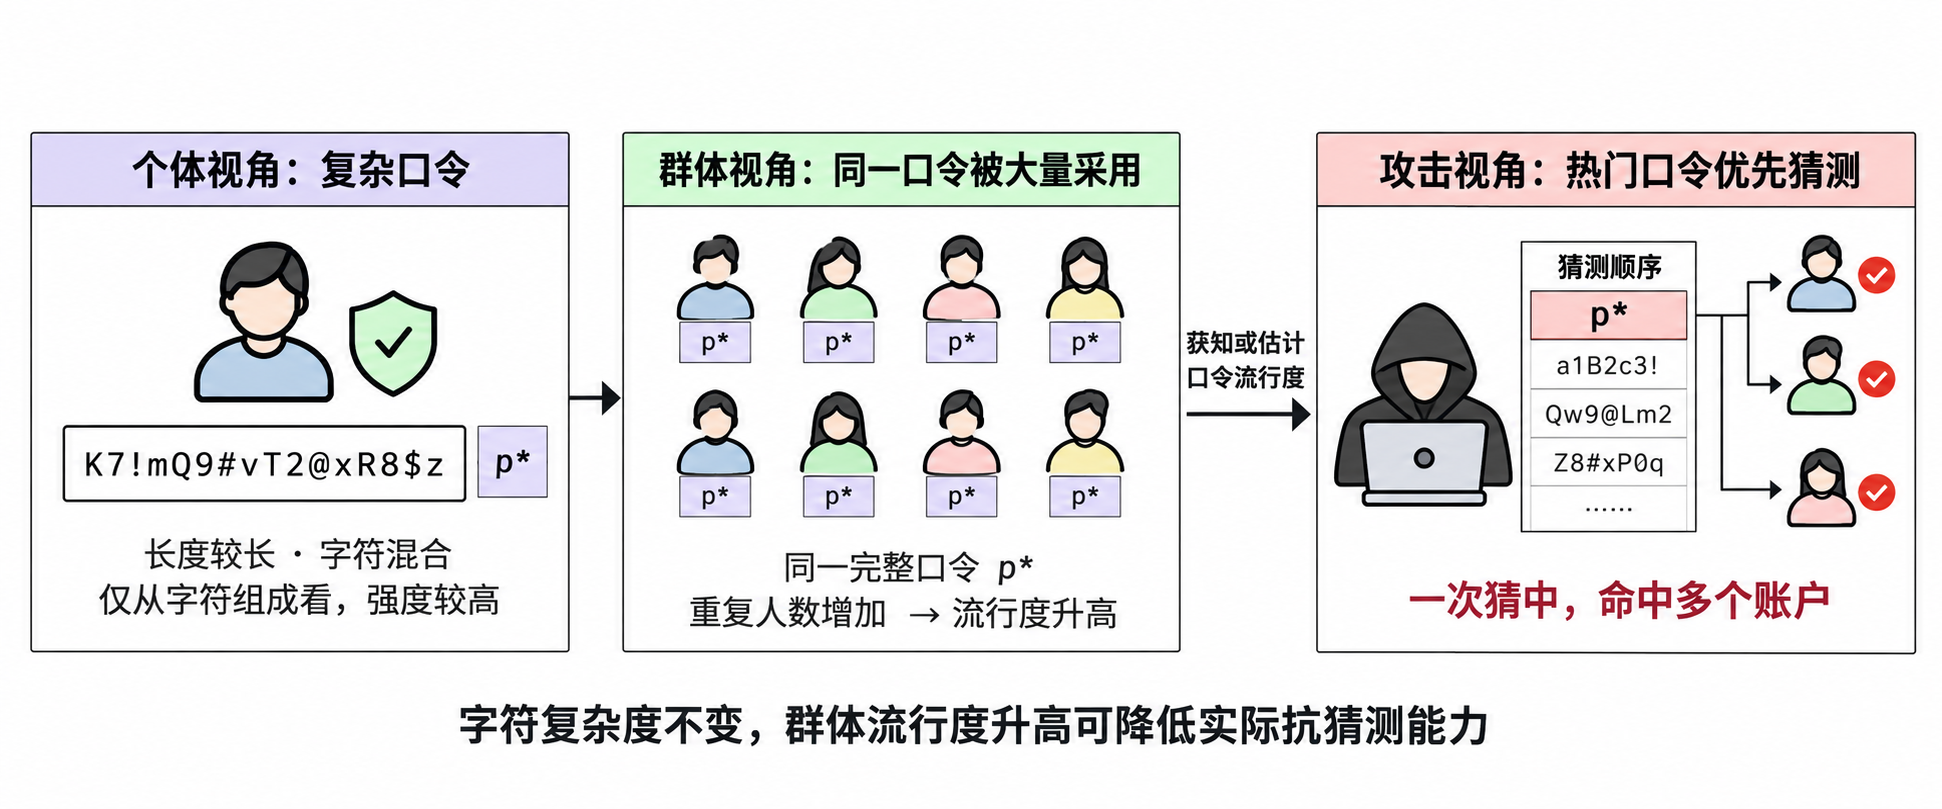
\includegraphics[width=\linewidth]{1-1.png}
\caption{\quad 口令被群体重复采用后的猜测风险示意}
\label{fig:password-popularity-risk}
\end{figure}

\subsection{相关工作}\label{sec:related-work}

\par\smallskip
\noindent\textbf{（1）分布评估与已有账户修改}
\nopagebreak[4]

Wang等用PDF-Zipf和CDF-Zipf描述口令频次与排名的关系，Hou与Wang进一步比较拉伸指数等拟合形式\cite{wang2017zipf,hou2023observations}。Johnson等提出Skeptic，模拟用户在不同组成要求下重新选择口令，以分布均匀程度比较政策，并利用拟合模型减少对原始口令数据的直接访问\cite{johnson2020skeptic}。

Xiao和Zeng提出HTPG，按Zipf曲线划分高频与低频口令，比较两类特征并生成修改建议，执行后周期性重新分类\cite{xiao2022zipf}。朱浩等提出FEPG，在频率之外加入口令字符熵，通过四类划分生成修改建议，并用PCFG评价模拟修改后的猜测效果\cite{zhu2023fepg}。\textbf{本作品进一步研究通知人数预算内的修改对象、要求和规模选择，以及执行后的反馈更新}。

\par\smallskip
\noindent\textbf{（2）热门口令与字符结构限制}
\nopagebreak[4]

Schechter等用count-min sketch估计口令使用频次，拒绝过于常见的口令\cite{schechter2010popularity}；Malone和Maher按频率进行概率性拒绝，引导选择分布趋于均匀\cite{malone2012distribution}。Komanduri等和Tan等通过用户研究比较组成、长度、强度与阻断名单等要求\cite{komanduri2011people,tan2020minimumstrength}。Segreti等研究包括PathWell在内的结构策略，将口令按字母、数字和符号的连续段编码，限制常见结构，同时评价猜测效果和创建负担；结构策略实验采用预先生成的名单模拟不同阶段\cite{segreti2017diversify}。\textbf{本作品从同一固定名单出发，根据近期注册情况和用户重选后的双模型攻击结果，确认后更新要求，并保留恢复原始名单的选项}。

\par\smallskip
\noindent\textbf{（3）隐私统计与口令检查}
\nopagebreak[4]

Blocki等对不附带字符串的口令排序频次加入噪声，保护统计发布\cite{blocki2016frequency}。Naor等结合安全两方计算与持续发布的差分隐私，私密发现热门口令并形成动态阻断名单，其协议考虑恶意参与者\cite{naor2019password}。Skeptic和PathWell也研究了减少明文访问或保存的方法\cite{johnson2020skeptic,segreti2017diversify}。\textbf{本作品保留字符结构与结构内匿名热门频次的对应关系，用于减少联合限制的重复覆盖，并由三方执行隐藏名单检查}。

攻击评价方面，PCFG学习口令结构与片段，OMEN按马尔可夫模型生成有序猜测，神经网络则学习更广泛的选择规律\cite{weir2009pcfg,durmuth2015omen,melicher2016neural}。猜测结果受模型、训练数据和配置影响\cite{ur2015guessability}，\textbf{本作品采用PCFG与OMEN，同时报告单模型和联合命中率}。

\subsection{作品概览}\label{ux4f5cux54c1ux6982ux89c8}

% Section 1.3 only; local evidence record: report_update/overview_1_3/claims.csv
本作品面向网站的口令管理，围绕“现有口令集调整分布、新注册用户怎样选取、口令不公开时怎样完成统计与检查、网站和用户怎样使用”四个问题，形成“已有口令集分布动态调整方案”、“模拟注册阶段口令策略动态调整方案”、“面向动态策略口令状态统计中的隐私保护方案”、“网站口令管理助手与用户口令辅助选取工具”四个部分。四部分的关系如图\ref{fig:triguard-overview}所示。

\begin{figure}[H]
\centering
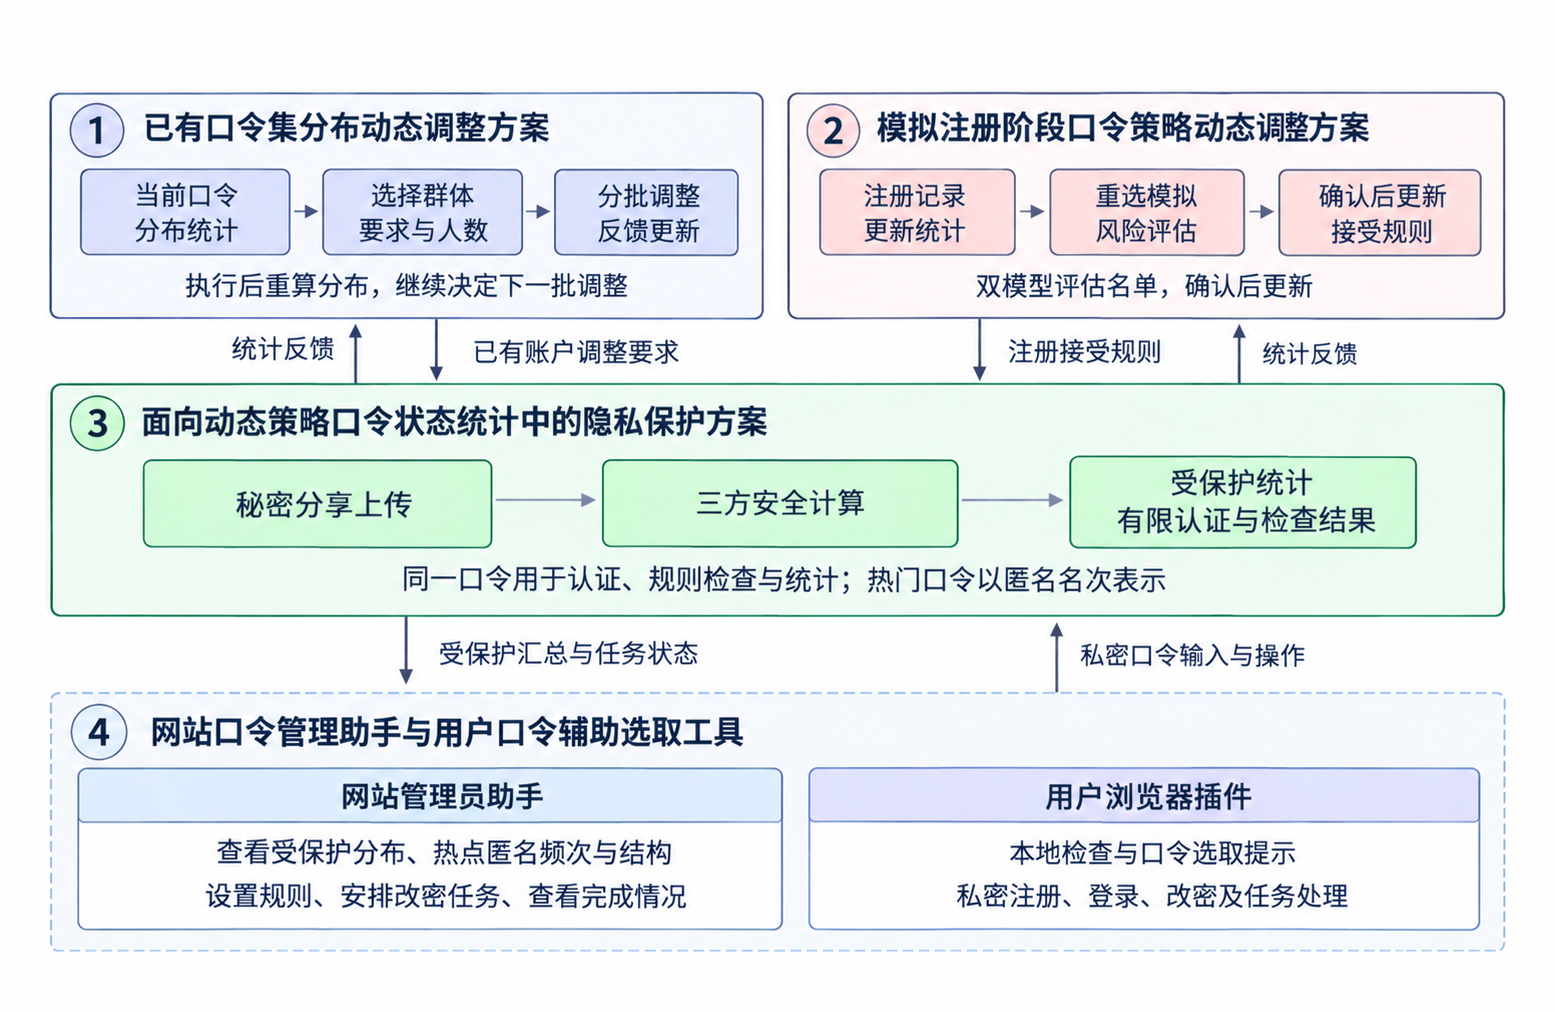
\includegraphics[width=\linewidth]{for1-2.png}
\caption{\quad TriGuard:局部动态口令优化系统}
\label{fig:triguard-overview}
\end{figure}

\subsubsection{面向已有账户改密的动态调整方案}\label{sec:overview-existing}

本作品提出面向已有账户的分批调整方法，将“修改哪些账户、采用什么要求、通知多少人”一起决定。在已有按频次识别高风险口令、生成修改建议的思路上，进一步加入通知人数限制和执行后的分布反馈，使有限的修改机会用于当前最值得处理的群体。

具体做法是统计完整口令的使用频次，结合口令结构生成候选群体与修改要求，再预测各方案能让分布变得多分散。候选新口令还需通过PCFG和马尔可夫猜测模型的检查。每轮执行后重新统计分布、更新剩余通知人数，并据此选择下一轮动作。

在相同通知人数的已有模拟比较中，该方法比一次排序和随机选人获得更分散的口令分布，双模型猜测命中率也更低。这一结果支持根据实际变化逐轮调整。

\subsubsection{面向新用户注册的动态调整方案}\label{sec:overview-registration}

本作品采用以Segreti结构名单为基础、经双模型确认更新的动态整类结构阻断方法。首批即执行完整的基础名单，后续根据最近注册者的使用情况提出新增结构限制。每次评估同时保留当前名单和原始名单，使系统既能继续使用当前要求，也能撤去效果不佳的新增限制。

名单更新前，先模拟用户被拒绝后的重选，再用PCFG与马尔可夫模型OMEN评估历史账户及下一批账户的累计猜测风险。新增名单在选择和另一组预览确认中均优于可行基准，才用于后续注册；只要联合命中率有正向改善即可采用。同批注册期间名单固定，模拟用户持续重选至接受，不设置修改次数上限。

第\ref{sec:validation-registration}节的10万模拟用户实验中，PCFG与OMEN各实际猜测100万次时，本作品方法的联合命中率为8.992\%，低于固定Segreti名单的9.431\%，少猜中439个账户。在相同样本和预算下，本方法的PCFG、OMEN及联合命中率均低于本节四个外部对照。

\subsubsection{口令统计与规则检查的隐私保护方案}\label{sec:overview-privacy}

为使前两类策略不依赖网站收集明文，本作品在已有秘密分享、安全计算和差分隐私方法上，增加结构内的匿名频次统计，并将认证、规则检查与统计更新连接起来。客户端将口令转换为三份随机份额，分别交给三个计算方；口令结构由同一秘密输入推导，管理员只获得加噪后的结构人数和热门口令的匿名频次。

热门完整口令及其真实排名对应关系保留在安全计算内部，注册或改密时可以据此检查，无须向网站公开名单。选择联合限制时，已被结构规则覆盖的热点不再重复占用完整口令名额；改密成功后撤销旧统计并加入新统计。由此建立了从私密输入、受保护统计到规则执行的处理链，适用于客户端可信、计算方按协议执行且不发生两方串通的场景。

\subsubsection{网站口令管理助手与用户口令辅助选取工具}\label{sec:overview-tool}

本作品制作了“网站口令管理助手与用户口令辅助选取工具”。网站管理员通过网站助手查看当前受保护的口令分布、热门口令的匿名名次与频次，以及热门结构汇总，并设置注册要求、安排已有账户改密任务、查看实际完成情况。界面不提供真实口令字符串或逐账户结构。

用户通过浏览器插件获得口令选取提示，先在本地检查公开要求，再通过私密检查确认是否符合本站隐藏规则，并完成注册、登录或改密。两端通过三方服务交换必要结果，形成“查看分布—制定要求—指导选取—反馈更新”的使用流程。
\subsection{作品贡献}\label{ux4f5cux54c1ux8d21ux732e}

\textbf{提出了面向已有账户改密的动态调整方案。}将需要修改的账户群体、修改要求和通知人数一起选择，在通知人数限制内预测各方案对整体口令分布的影响，并用PCFG与马尔可夫猜测模型检查修改后的个体口令。每轮执行后重新统计分布和剩余通知人数，再制定下一轮方案，将群体分布改善、个体口令强度与通知成本结合起来。

\textbf{提出了面向新用户注册的动态调整方案。}从完整Segreti结构名单开始，始终保留原始名单和当前名单作为备选，依据近期使用情况提出新增限制。更新前模拟用户重选，用PCFG与OMEN评价累计猜测风险，并由另一组预览再次确认。以两次评价中的正向改善决定是否追加限制，也允许恢复原始名单，使规则调整直接服务于攻击抵抗效果。

\textbf{构建了口令统计与规则检查的隐私保护方案。}在已有秘密分享、安全计算和差分隐私方法上，补充按结构分组的匿名频次统计，模拟管理员能够查看热门结构及结构内的热门口令频次，并在选择完整口令限制时排除已被结构规则覆盖的部分。同时，将认证、规则检查和统计更新绑定到同一个秘密口令输入。在客户端可信、计算方按协议执行且不发生两方串通的前提下，网站可利用受保护统计制定要求，由三方服务执行隐藏口令检查。

\textbf{实现了网站口令管理助手与用户口令辅助选取工具。}管理员通过网站助手查看受保护的分布和结构汇总、设置口令要求、安排已有账户改密任务并跟踪完成情况；用户通过浏览器插件获得选取提示，进行本地公开规则检查和本站私密规则检查，并完成注册、登录与改密。两端通过三方服务交换必要结果，将统计、策略管理、用户选取和执行反馈连接为可运行的使用流程。
\subsection{应用场景与研究范围}\label{ux5e94ux7528ux573aux666fux4e0eux7814ux7a76ux8303ux56f4}

本作品面向采用口令登录的网站和组织，主要适用于已有账户口令调整与新用户注册两类场景。对于已有账户，管理员可在通知人数限制内确定优先处理的群体，分批安排改密，并根据口令分布的变化继续调整；对于新注册用户，可从已有结构限制出发，根据近期使用情况评估是否追加限制，以重选后的累计猜测风险决定更新。两类方法分别服务于已有口令的逐步改善和新口令的持续选取。

在需要保护用户口令隐私的接入场景中，网站通过管理助手查看受保护的统计汇总和任务状态，用户在浏览器插件内输入口令，由三方服务完成认证与规则检查，网站只接收必要结果。已有账户需在原网站确认用户身份后，通过助手重新登记秘密口令；原有加盐哈希不能直接作为完整口令频次统计的输入。隐私方案适用于客户端可信、计算方按协议执行且不发生两方串通的条件。

本作品已完成两类动态策略的模拟研究，并制作了可运行的双端工具原型。实验中的用户响应与重选行为由模型模拟，所得效果限于给定数据、规则范围、响应假设和猜测模型；已有账户调整保留通知人数预算，注册模拟则不设置修改次数硬上限。工具原型已在本地接通受保护统计、策略设置、注册、登录、改密与任务反馈，但尚未完成跨机构部署和大型网站容量验证。实际接入时，应结合本站用户行为与运行条件确认策略效果，缺少重选与成本依据时保持当前自动策略。
\clearpage
\section{作品设计与实现}\label{ux7b2cux4e8cux7ae0-ux4f5cux54c1ux8bbeux8ba1ux4e0eux5b9eux73b0}

\subsection{方案设计}\label{ux7cfbux7edfux65b9ux6848}

\subsubsection{面向已有账户改密的动态调整方案}\label{sec:design-existing}

本部分提出一种依据口令分布逐轮调整修改要求的算法，面向已经形成的口令集，在通知人数有限的情况下，决定哪些账户优先修改、采用什么要求、每轮通知多少人。算法输入包括当前账户及其口令、网站基础要求、可选修改规则和通知人数上限，输出为每轮的账户名单、对应规则、预计分布变化及实际执行记录。具体过程是先统计，再预测和比较不同修改安排，检查候选新口令，最后执行所选方案并重新统计。图\ref{fig:existing-dynamic-flow}展示动态调整方案的执行流程。

\begin{figure}[H]
\centering
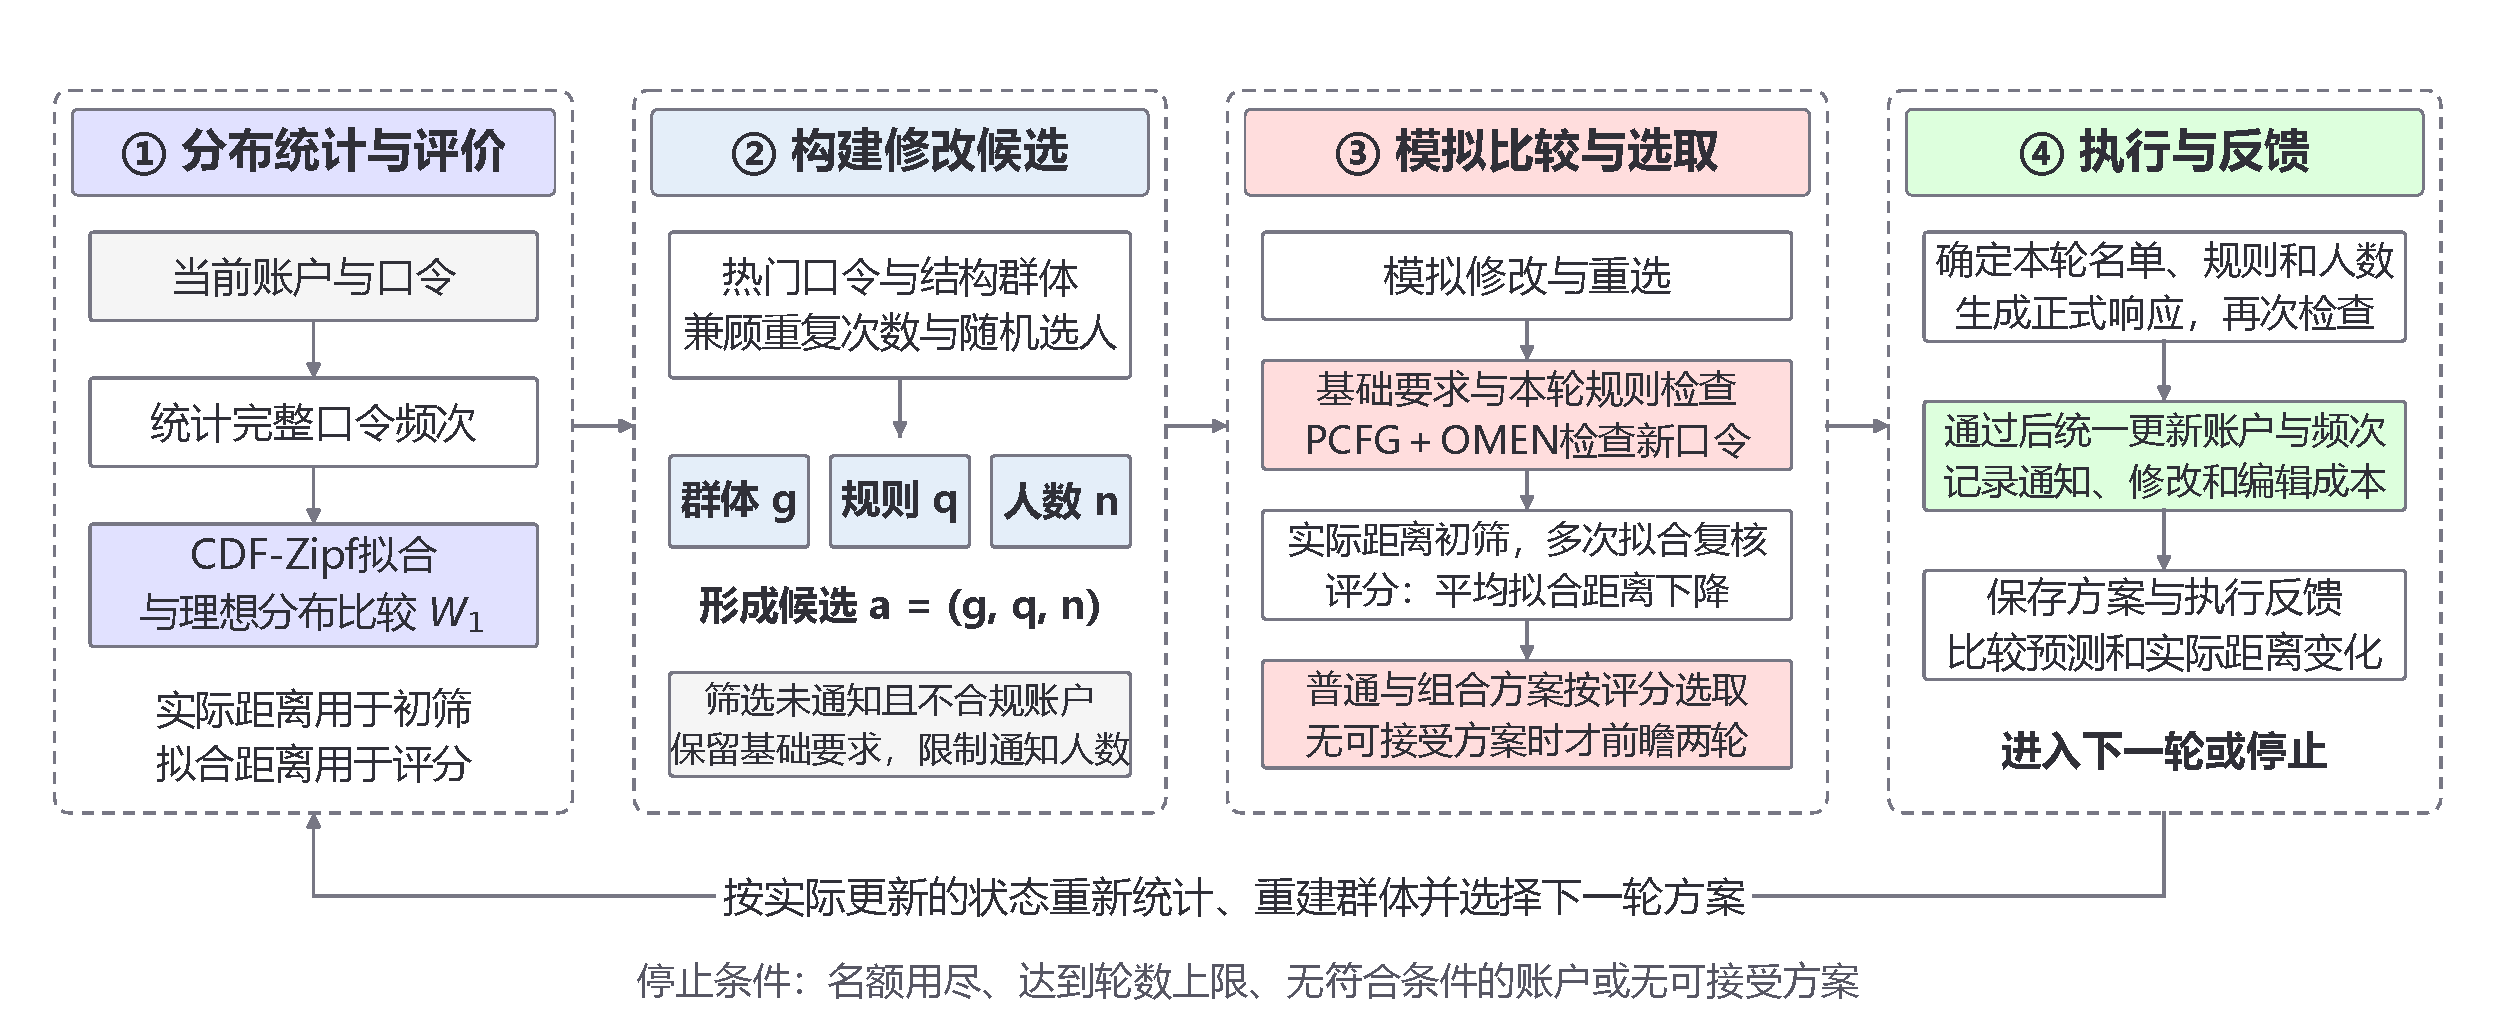
\includegraphics[width=0.99\textwidth]{existing-dynamic-overview-2-1-1.pdf}
\captionsetup{labelsep=space}
\caption{已有口令集分布动态调整方案的模块概览与反馈循环}
\label{fig:existing-dynamic-flow}
\end{figure}

\par\smallskip
\noindent\textbf{（1）统计分布并计算距离}
\nopagebreak[4]

以完整字符串统计口令频次。设账户总数为$N$，第$t$轮中排名第$r$的口令有$f_t(r)$个账户使用，概率为$f_t(r)/N$；不足$N$个排名的部分补零。将排名转为归一化对数坐标：

\[x_r=\frac{\ln r}{\ln N},\qquad r=1,\ldots,N,\quad N>1.\]

以“每个账户使用一个不同口令”为理想分布，即$N$个口令的频次均为1的均匀分布。记当前与理想分布的累计函数为$C_t(x)$和$C^*(x)$，用一维Wasserstein-1距离\cite{panaretos2019wasserstein}衡量两者差距：

\[D_t=W_1(P_t,P^*)=\int_0^1|C_t(x)-C^*(x)|\,\mathrm{d}x.\]

距离越小，完整口令的重复越少。算法先用实际频次计算的经验距离筛选候选，再用拟合距离进一步评分。

\par\smallskip
\noindent\textbf{（2）拟合并评价候选分布}
\nopagebreak[4]

采用两参数CDF-Zipf近似累计频次\cite{wang2017zipf}，便于反复拟合和采样。由$F(r)\approx cr^s$定义用于采样的连续辅助分布：

\[G(x)=\min\{cx^s,1\},\qquad x\geq0,\quad c,s\in(0,1].\]

程序通过实际排名与累计概率的对数回归确定初值，再用粗网格与有限次黄金分割搜索调整参数。对于给定的$c$和$s$，生成均匀随机数并取得类别编号：

\[R=\left\lfloor(U/c)^{1/s}\right\rfloor,\qquad U\sim\mathrm{Uniform}(0,1).\]

重复抽样$N$次，按类别计数并排序得到模拟频次，以它与实际频次的最大累计差为拟合误差。参数比较使用同一组随机数。选定参数后，再以三组独立于搜索阶段的随机数重新抽样，计算平均拟合距离：

\[\widehat D_t=\frac{1}{3}\sum_{m=1}^3 W_1(\widetilde P_t^{(m)},P^*).\]

\par\smallskip
\noindent\textbf{（3）构建修改候选}
\nopagebreak[4]

候选记为$a=(g,q,n)$，由账户群体$g$、修改规则$q$和通知人数$n$构成，并保存具体账户名单。群体包括热门完整口令的使用者、按字母数字符号结构划分的账户，以及不限定结构、按重复次数或随机选取的账户。

后续候选池包含18项要求，覆盖长度、字符类别、重复与连续序列，以及字典词、热门口令和泄露口令限制，完整目录见表\ref{tab:rule-catalogue}。网站基础要求始终保留，候选账户须违反对应规则且尚未接受本阶段通知；字典和泄露名单来自独立开发样本，热门名单随统计更新。

每种群体与规则配对按配置生成不同通知规模，人数受可选账户数、单轮上限和累计剩余额度约束。同一账户在后续调整阶段至多通知一次，基础与后续阶段分别计数。

\par\smallskip
\noindent\textbf{（4）模拟修改并选择方案}
\nopagebreak[4]

程序用局部修改、片段拼接和重新选取三种方式模拟用户响应。各候选对同一账户使用公共随机流，正式执行另用随机流。通过新口令检查后，从旧口令频次中减去修改人数，再加入新口令频次，得到候选执行后的分布。

先用经验距离初筛，再对入选候选进行$M$次响应模拟与拟合距离复核。设候选$a$第$m$次模拟后的拟合距离为$\widehat D_{t+1}^{(a,m)}$，评分为：

\[S(a)=\frac{1}{M}\sum_{m=1}^M[\widehat D_t-\widehat D_{t+1}^{(a,m)}].\]

在人数符合预算、全部新口令通过检查且收益超过数值容差的候选中，选择评分最高者；同分时依次比较热门部分占比的下降和通知人数。

\par\smallskip
\noindent\textbf{（5）检查新口令}
\nopagebreak[4]

新口令须不同于旧口令，满足基础要求与本轮规则，并通过固定PCFG和马尔可夫模型OMEN的检查\cite{weir2009pcfg,durmuth2015omen}。参考百万次猜测门槛的研究\cite{florencio2014password,tan2020minimumstrength}，预先生成两个模型各自前$10^6$次实际猜测，建立查询表。候选至少处于一个模型的支持范围，且在两个表中均未命中时通过；重复输出计入猜测次数。

\par\smallskip
\noindent\textbf{（6）比较组合与两轮安排}
\nopagebreak[4]

不同要求可以分配给互不重叠的账户，组成同一批次，并按总人数和完整批次重新模拟、检查和评分。单轮候选与组合均无可接受收益时，程序在剩余预算和轮数内预览少量连续两轮的安排。

预览先执行首轮，再按新状态选择第二轮。首轮允许配置范围内的暂时分布损失，全部新口令仍需通过检查；每次预演的两轮合计收益都须超过容差。选择平均两轮收益最大的首轮方案，实际执行后再根据新状态决定下一轮。

\par\smallskip
\noindent\textbf{（7）执行并更新}
\nopagebreak[4]

正式执行前重新生成响应，核对账户、旧口令、规则与整批新口令。通过后统一更新账户、频次和成本，再按新状态重建候选。每轮保存所选群体、要求、人数、预测距离和实际变化；预算或轮数用尽、无合适账户，或当前搜索与两轮预览均无可接受方案时停止。



\subsubsection{面向新用户注册的动态调整方案}\label{sec:design-registration}

本部分提出以Segreti结构名单为基础、经双模型确认更新的动态整类结构阻断方法。系统从首批就执行完整基础名单，后续根据近期注册情况尝试增加限制，但每轮都保留原始名单与当前名单作为可选方案。新增限制只有在两组预览中都降低累计联合命中率才启用；若新增要求没有价值，可以保持现状或恢复原始名单。这样，规则是否变严取决于用户重选后的攻击效果。图\ref{fig:registration-dynamic-overview}展示候选构造、重选风险评价、独立确认与执行反馈的流程。

\begin{figure}[H]
\centering
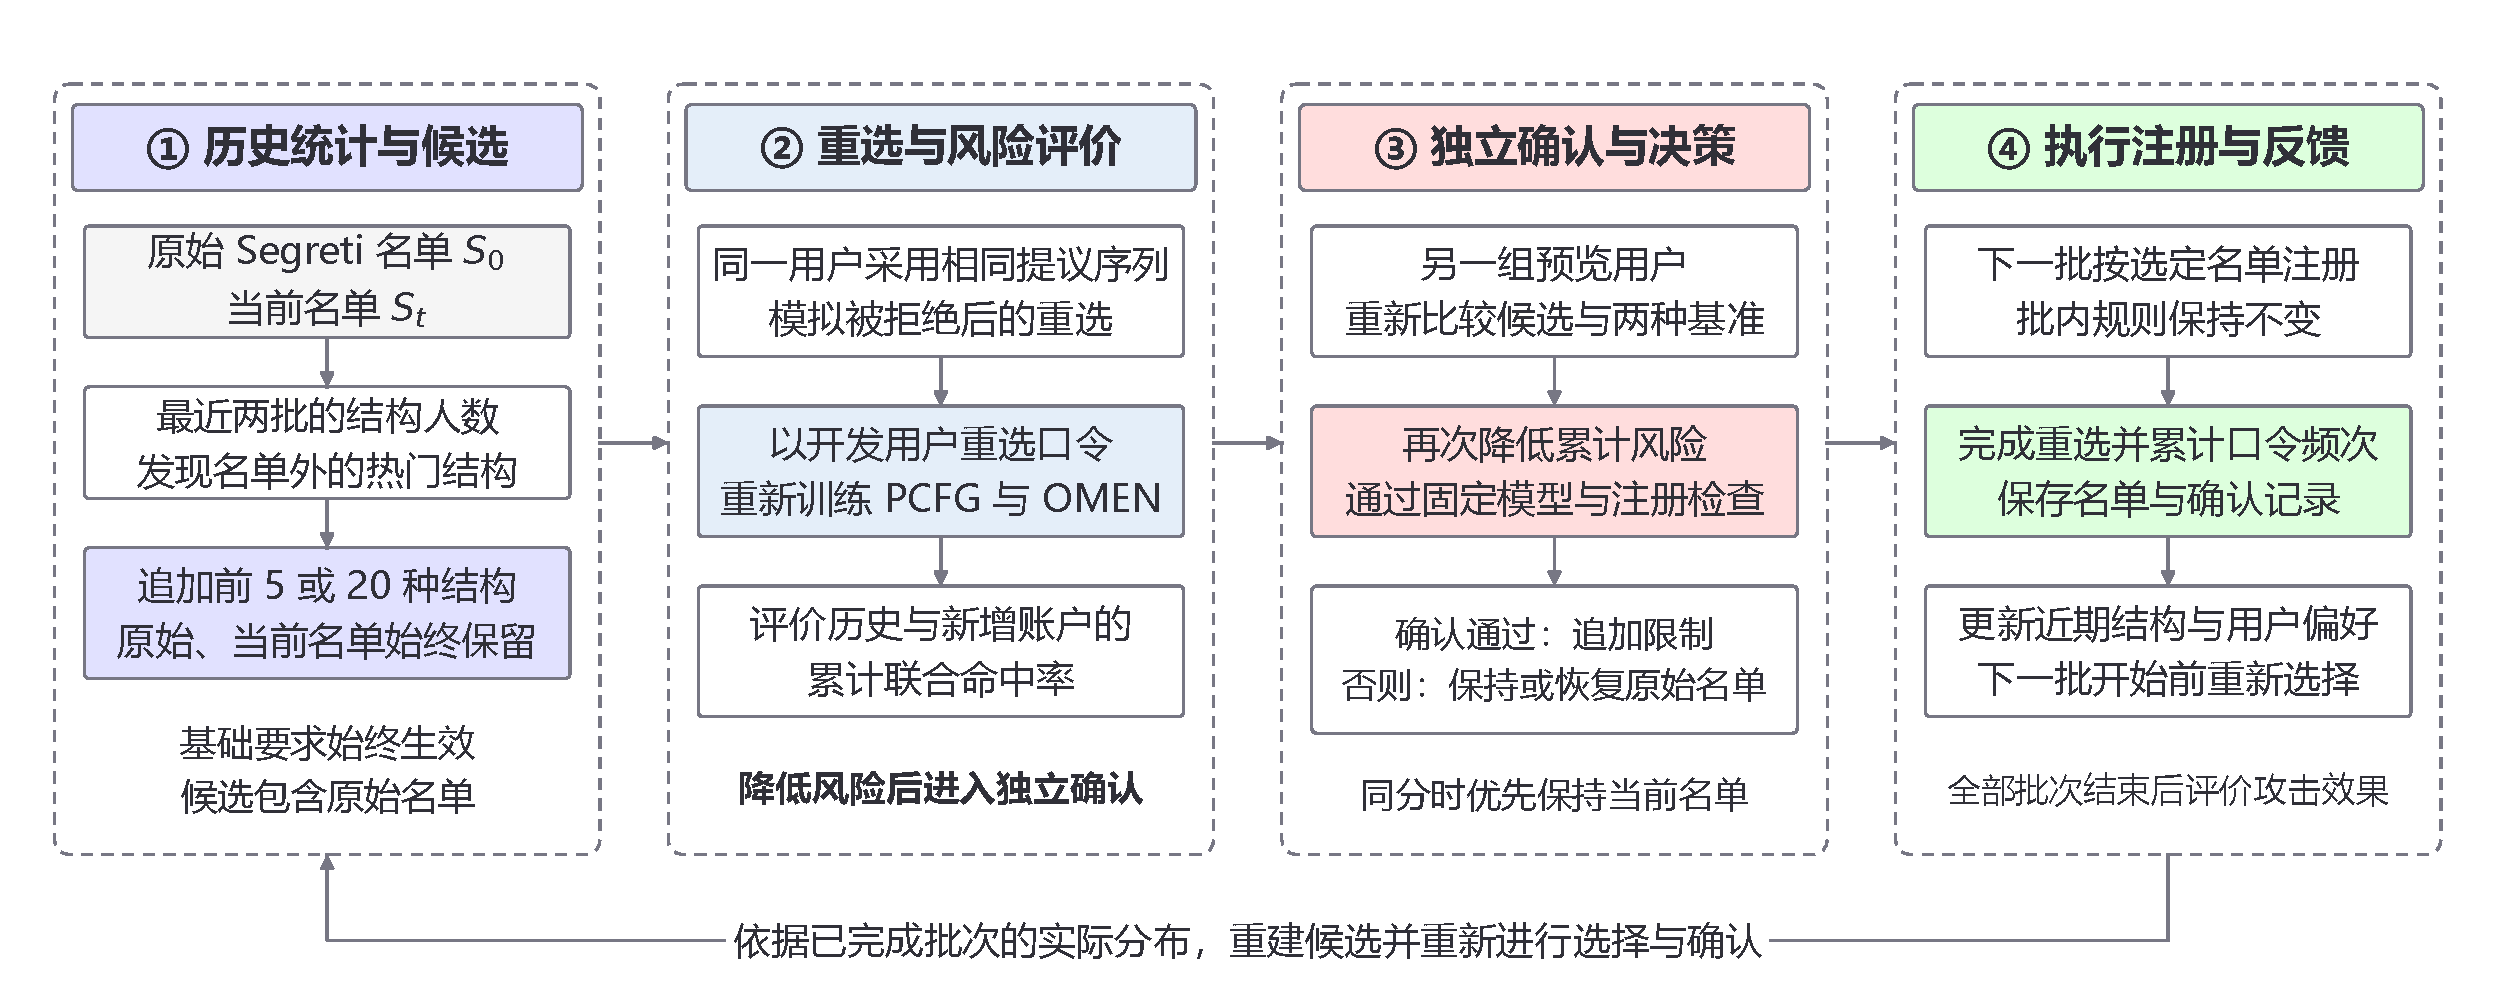
\includegraphics[width=0.99\textwidth]{registration-dynamic-overview-2-1-2.pdf}
\captionsetup{labelsep=space}
\caption{面向新用户注册的动态调整方案的模块概览与反馈循环}
\label{fig:registration-dynamic-overview}
\end{figure}

\par\smallskip
\noindent\textbf{（1）建立基础要求与原始名单}
\nopagebreak[4]

基础要求$P_0(w)$为至少8位，并拒绝开发训练样本中最常见的1,000个口令。从开发PCFG前10万个满足要求的不同猜测中提取结构，形成原始名单$S_0$，共213种；动态方法与固定Segreti对照加载同一名单，从首批执行。

程序保存累计频次、最近两批频次及用户首次提议，分别用于整体风险评价、新增热点发现和下一批偏好估计。控制器只读取已完成批次，新要求作用于后续注册。

\par\smallskip
\noindent\textbf{（2）构造新增结构名单}
\nopagebreak[4]

字符结构$\phi(w)$按连续字符的类别与长度编码，L、U、D、S分别表示小写字母、大写字母、数字和其他字符。例如，六个小写字母、四个数字和一个符号对应L6D4S1。

每轮保留原始名单$S_0$和当前名单$S_t$，统计最近两批中满足原始要求的结构人数：

\[n_t(s)=\sum_{\phi(w)=s}h_t(w).\]

在尚未被相应名单覆盖、使用人数不少于20的结构中，按人数降序排列，同人数按编码排序；分别在两种名单之外尝试追加前5种或前20种结构，可用数量不足时全部选取，相同候选合并。候选始终包含$S_0$，接受条件为：

\[A_S(w)=P_0(w)\land[\phi(w)\notin S].\]

名单在同一批注册期间固定，下一批开始前更新；恢复原始名单时撤去动态追加的部分。

\par\smallskip
\noindent\textbf{（3）模拟用户重选}
\nopagebreak[4]

每名模拟用户的提议序列由标识和随机种子确定。被拒绝后，按局部修改、片段拼接和重新选取继续尝试，取第一个满足要求的口令。不同候选对同一用户使用相同序列，选择与确认使用不同预览角色；下一批偏好由开发预览记录与历史首次提议各占一半估计。模拟设定为持续尝试至接受，具体比例和规模见附录\ref{app:registration-reproduction}。

\par\smallskip
\noindent\textbf{（4）评价累计攻击风险}
\nopagebreak[4]

候选作用于独立开发用户后，以其重选口令训练PCFG与OMEN\cite{weir2009pcfg,durmuth2015omen}，使攻击者学习替代口令的规律。训练保留此前各批的开发口令并加入新批口令，目标和预览用户用于评价。

设已有$N_t$个账户，历史分布为$H_t$，下一批人数为$m$，候选$a$的预览分布为$Q_t^a$。以$r_B^\cup(D;a)$表示相应双模型各猜测$B$次时，分布$D$中至少被一个模型猜中的账户比例，累计风险为：

\[\widehat R_t^\cup(a)=\frac{N_t r_B^\cup(H_t;a)+m r_B^\cup(Q_t^a;a)}{N_t+m}.\]

选择、确认和最终评价均取$B=10^6$，联合最多200万次尝试；重复猜测计入预算，重复命中的账户计一次。评价同时包含历史与新增账户，记录实际完成次数及两模型均不支持的比例。

\par\smallskip
\noindent\textbf{（5）检查重选后的风险变化}
\nopagebreak[4]

用原始开发训练口令建立固定双模型，各生成前100万次猜测，取并集$F$。候选与本轮原始名单的预览结果比较：在$F$中的命中比例增量不超过0.5个百分点，两模型均不支持的比例增量不超过2个百分点，并完成全部模拟注册。

\par\smallskip
\noindent\textbf{（6）确认后更新名单}
\nopagebreak[4]

选择阶段以原始和当前名单中累计风险较低的可行方案为基准，新增候选降低风险后进入确认。确认阶段用另一组用户重新比较候选与两种基准；新增名单再次降低风险并通过检查后启用，否则采用更好的基准。收益用$10^{-12}$容差判断。

同分时依次比较重复程度、人均额外提交和名单大小，并优先保持当前名单。两次比较共同决定本轮追加、保持或恢复。

\par\smallskip
\noindent\textbf{（7）执行注册与最终评价}
\nopagebreak[4]

每批按选定名单完成注册，将成功口令加入累计频次，保存名单与确认记录。开发用户也按相同流程逐批重选。全部注册结束后，以各方案的开发重选口令训练最终双模型，按指定预算评价全部100,000条初始目标记录，报告单模型和联合命中率。

\subsubsection{口令统计与规则检查的隐私保护方案}\label{sec:design-privacy}

前两部分研究了如何根据口令分布安排已有账户改密，以及如何调整注册要求。实际网站要采用这些方法，还需要解决一个问题：怎样在不收集明文口令的情况下，获知口令是否过于集中，并执行相应限制。本部分为此设计了“私密上传—匿名统计—联合规则—私密检查—成功后更新”的处理流程。管理员依据受保护的群体统计选择限制，真实口令及其对应关系保留在秘密计算中。图\ref{fig:privacy-protection-overview}展示私密输入、三方统计、受保护发布与私密检查更新的流程。

\begin{figure}[H]
\centering
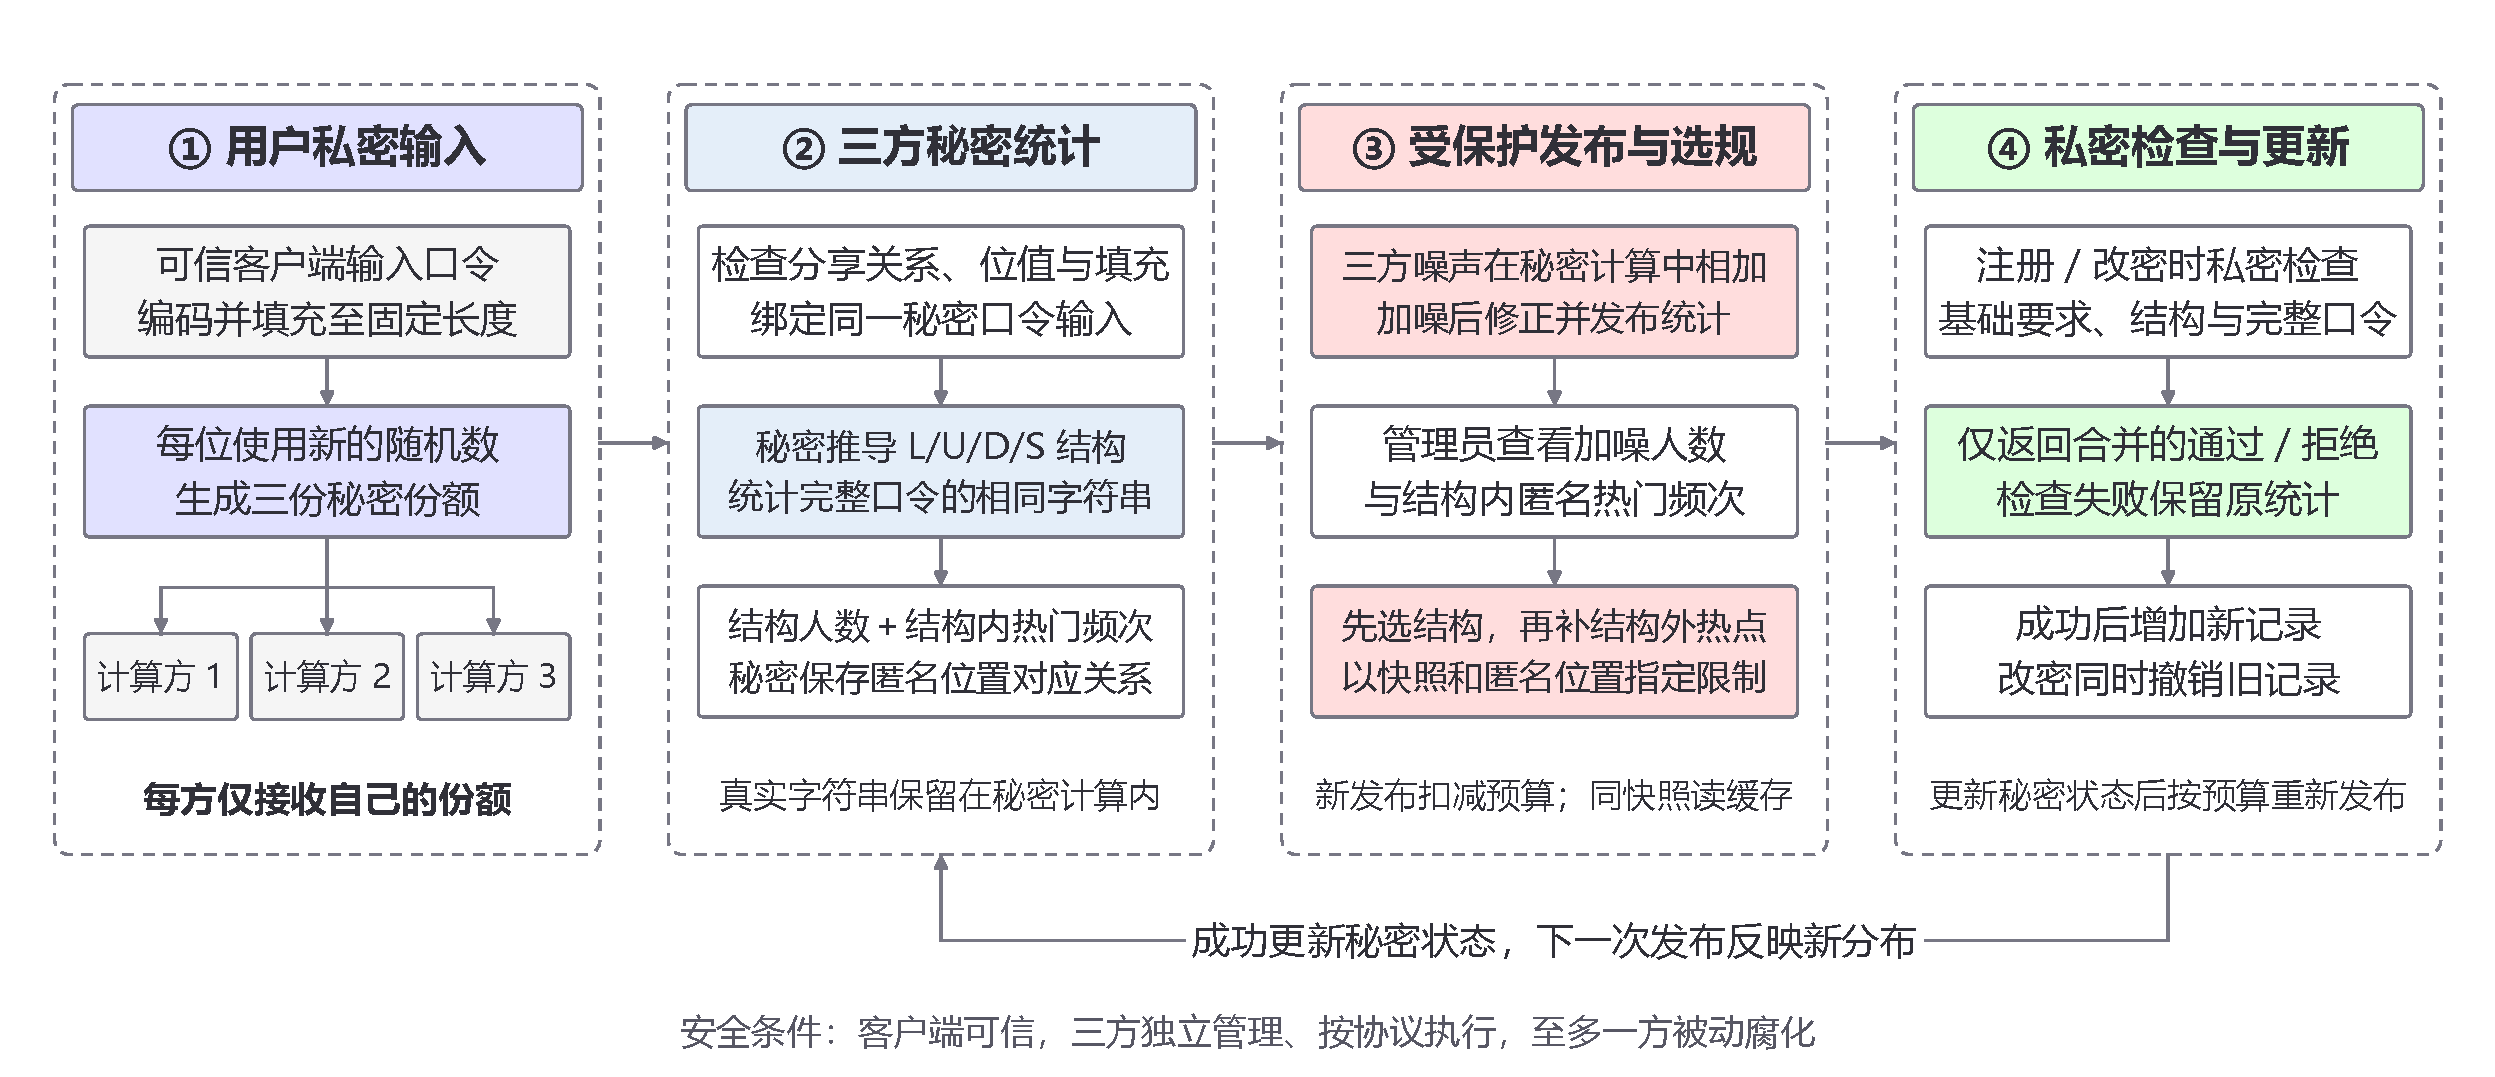
\includegraphics[width=0.99\textwidth]{privacy-protection-overview-2-1-3.pdf}
\captionsetup{labelsep=space}
\caption{口令统计与规则检查的隐私保护方案流程}
\label{fig:privacy-protection-overview}
\end{figure}

秘密分享、安全计算和差分隐私采用已有方法\cite{shamir1979secret,benor1988mpc,dwork2014privacy}。

\par\smallskip
\noindent\textbf{（1）参与方与安全条件}
\nopagebreak[4]

用户通过可信客户端将口令转换为随机份额，三个计算方各接收一份，共同完成口令比较、结构推导、规则检查与统计。管理员获得加噪的结构人数和匿名频次，并选择相应限制。

通信经过认证并加密，三方由独立主体控制。计算方按协议执行，至多一方受攻击者控制并记录自身收到的信息；任意两方持有的份额可恢复秘密。

\par\smallskip
\noindent\textbf{（2）分享口令并绑定检查输入}
\nopagebreak[4]

口令编码后补齐到固定长度，再逐位分享，使份额数量保持一致。对每一位$b\in\{0,1\}$，在有限域$\mathbb F_p$中独立均匀选择随机数$a$，其中$p>3$为素数，生成：

\[y_i=(b+ai)\bmod p,\qquad i=1,2,3.\]

对固定的$b$和$i$，映射$a\mapsto b+ai$是一一对应的，因此单份额均匀分布，且与$b$无关：

\[\Pr[y_i=z\mid b=0]=\Pr[y_i=z\mid b=1]=\frac1p,\qquad z\in\mathbb F_p.\]

每位和每次输入使用新的随机数。三方先检查分享关系、二进制位、字符范围和连续填充，再将同一秘密字符用于口令比较、结构推导、规则判断和频次更新。各方以独立保密密钥生成HMAC\cite{rfc2104hmac}，绑定输入与本次请求。

\par\smallskip
\noindent\textbf{（3）按结构保存匿名频次}
\nopagebreak[4]

结构采用L/U/D/S连续段编码，由秘密字符推导。完整口令按相同字符串计数；对公开结构目录$\mathcal S$中的每个结构$s$，保存账户人数$n_s$和该结构内前$L$个排序频次，不足项补零：

\[F_s=(f_{s,1},\ldots,f_{s,L}),\qquad V=((n_s,F_s))_{s\in\mathcal S}.\]

它同时描述结构的使用人数和其中的完整口令重复程度。保留归属关系有助于计算两类限制的共同影响：例如，两组数据的全局频次均为$(4,3,2,1)$，结构A、B各5人；若A内频次为$(4,1)$、B内为$(3,2)$，禁止A或第一热门口令覆盖5人；两者交换后覆盖9人。

管理员取得加噪人数、匿名名次与频次。三方内部保存“结构、匿名位置、秘密口令”的对应关系，并绑定本次统计结果，供规则检查使用。结构目录与每类保留的频次数量在发布前固定，其余结构归入OTHER，用于完整口令频次统计。

\par\smallskip
\noindent\textbf{（4）加噪后发布统计}
\nopagebreak[4]

差分隐私通过加入噪声限制统计对个人选择的暴露\cite{blocki2016frequency,dwork2014privacy}。相邻状态定义为账户人数固定、替换一个账户口令。结构人数与结构内排序频次的绝对变化总和分别至多为2，核心统计的敏感度满足：

\[\Delta_1(V)\leq4.\]

各方独立产生噪声，在秘密计算内相加后发布，再修正负数、频次顺序与人数范围。修正属于差分隐私后处理。有限采样采用$(\varepsilon,\delta)$近似差分隐私，尾项配置见第\ref{sec:validation-privacy-4}节。若同时发布规则违反人数，需按这部分统计的敏感度分配独立预算。

每次发布新的带噪统计均计入累计预算，读取同一已发布结果沿用原值；用于分析和确认的两次发布分别消耗预算。

\par\smallskip
\noindent\textbf{（5）构造并检查隐藏联合限制}
\nopagebreak[4]

设禁止结构集合为$T$，完整口令集合为$B$，结构$s$中使用$B$内口令的人数为$E_s(B)$，共同覆盖人数为：

\[R(B,T)=\sum_{s\in T}n_s+\sum_{s\notin T}E_s(B).\]

先选择至多$j$个被禁结构，再从其他结构中补充至多$k$个热门完整口令，减少重复覆盖。选择依据是已发布的带噪人数与频次，完整口令以结构和匿名位置指定。三方根据对应的统计结果找到秘密字符串，共同检查输入是否满足基础要求、避开被禁结构和完整口令，返回合并的通过或拒绝结果。OTHER仅用于完整口令位置选择。

在精确频次、结构集合已确定且$k\leq L$时，各桶前$L$项包含结构外的前$k$项，选最大频次可取得最大额外覆盖。

\par\smallskip
\noindent\textbf{（6）更新秘密统计}
\nopagebreak[4]

每个账户以当前口令贡献一条记录。账户加入时增加记录，口令修改成功后撤去旧记录并加入新记录，账户退出时撤去记录。完整口令频次、所属结构人数及排序频次均在秘密计算内更新；检查失败时保留原值。下一次发布据此重新生成带噪统计，供后续规则选择使用。

\subsection{作品实现}\label{sec:implementation-tools}

本作品将已有口令分批调整、注册阶段策略调整和口令隐私保护三项方案接成可运行的双端系统，命名为TriGuard。网站管理员使用管理网站，负责查看群体口令情况、制定要求和跟踪改密；用户使用浏览器插件，负责选取口令、完成账户操作和处理本人的任务。管理员网站以全站账户为管理对象，提供统计、策略与任务分配入口；用户插件以本人账户为操作对象，提供口令输入、检查反馈与任务处理入口。两端通过后端交换公开策略、本人任务和受保护汇总，分别使用自己的登录身份和权限。

\begin{figure}[H]
\centering
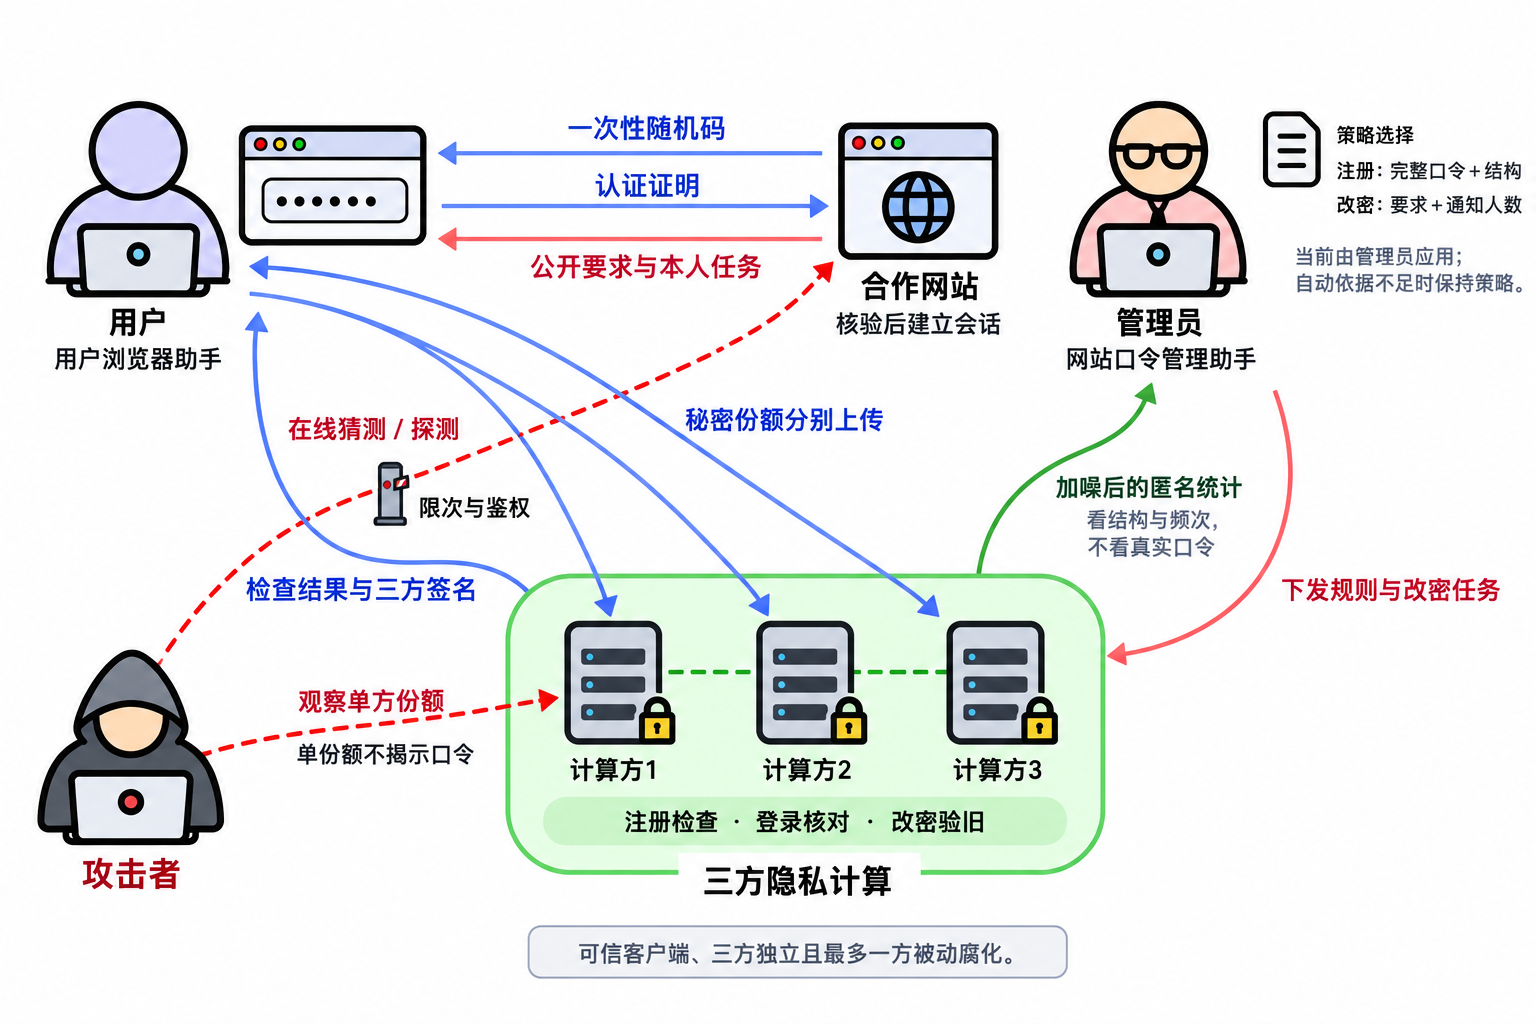
\includegraphics[width=0.94\linewidth,height=0.72\textheight,keepaspectratio]{tool-principle-icons-2-2.png}
\caption{\quad 双端工具与三方计算的交互示意图}
\label{fig:tool-principle}
\end{figure}

\subsubsection{双端系统组成与运行流程}\label{sec:implementation-composition}

系统由管理员网站、用户浏览器插件、两类业务服务和三个计算方组成，交互关系见图\ref{fig:tool-principle}。两个前端采用React和TypeScript开发，管理员端以网页运行，用户端打包为Chromium浏览器扩展；业务服务采用Python和FastAPI，三个计算方使用MPyC共同完成口令比较、规则检查和统计\cite{mpycsoftware}。业务服务保存策略版本、账户版本、会话及任务状态，各计算方分别保存自己的口令份额。

一次完整使用过程从管理员查看当前统计开始。管理员选择注册要求或已有账户的改密要求，用户插件读取生效策略并提示用户；用户在插件内完成注册或改密，成功结果经过三方核验后更新账户、任务和当前统计贡献。管理员随后查看任务进展，需要了解新的群体分布时再发布统计快照。管理员的全站工作台见图\ref{fig:tool-admin-overview}，用户的个人检查界面见图\ref{fig:tool-user-feedback}。前者可以制定网站要求并汇总任务进展，后者读取已生效要求、检查本人输入并执行账户操作，形成从策略到用户响应的完整流程。

管理员首先在“运行总览”确认当前策略、任务进度和计算服务状态，如图\ref{fig:tool-admin-overview}所示。图中的生效策略为版本6，口令长度为12至64字符；82项已完成、102项已分配是站点累计任务状态，包含本次100人合成账户流程和原有2项已完成任务。这里用这些数字说明进度页面的含义，具体实验设置和效果分析放在第三章。三个计算方的“就绪”标识表示服务可用；本机演示运行三个进程，实际隐私部署仍需满足2.1.3规定的独立计算方条件。

\begin{figure}[H]
\centering
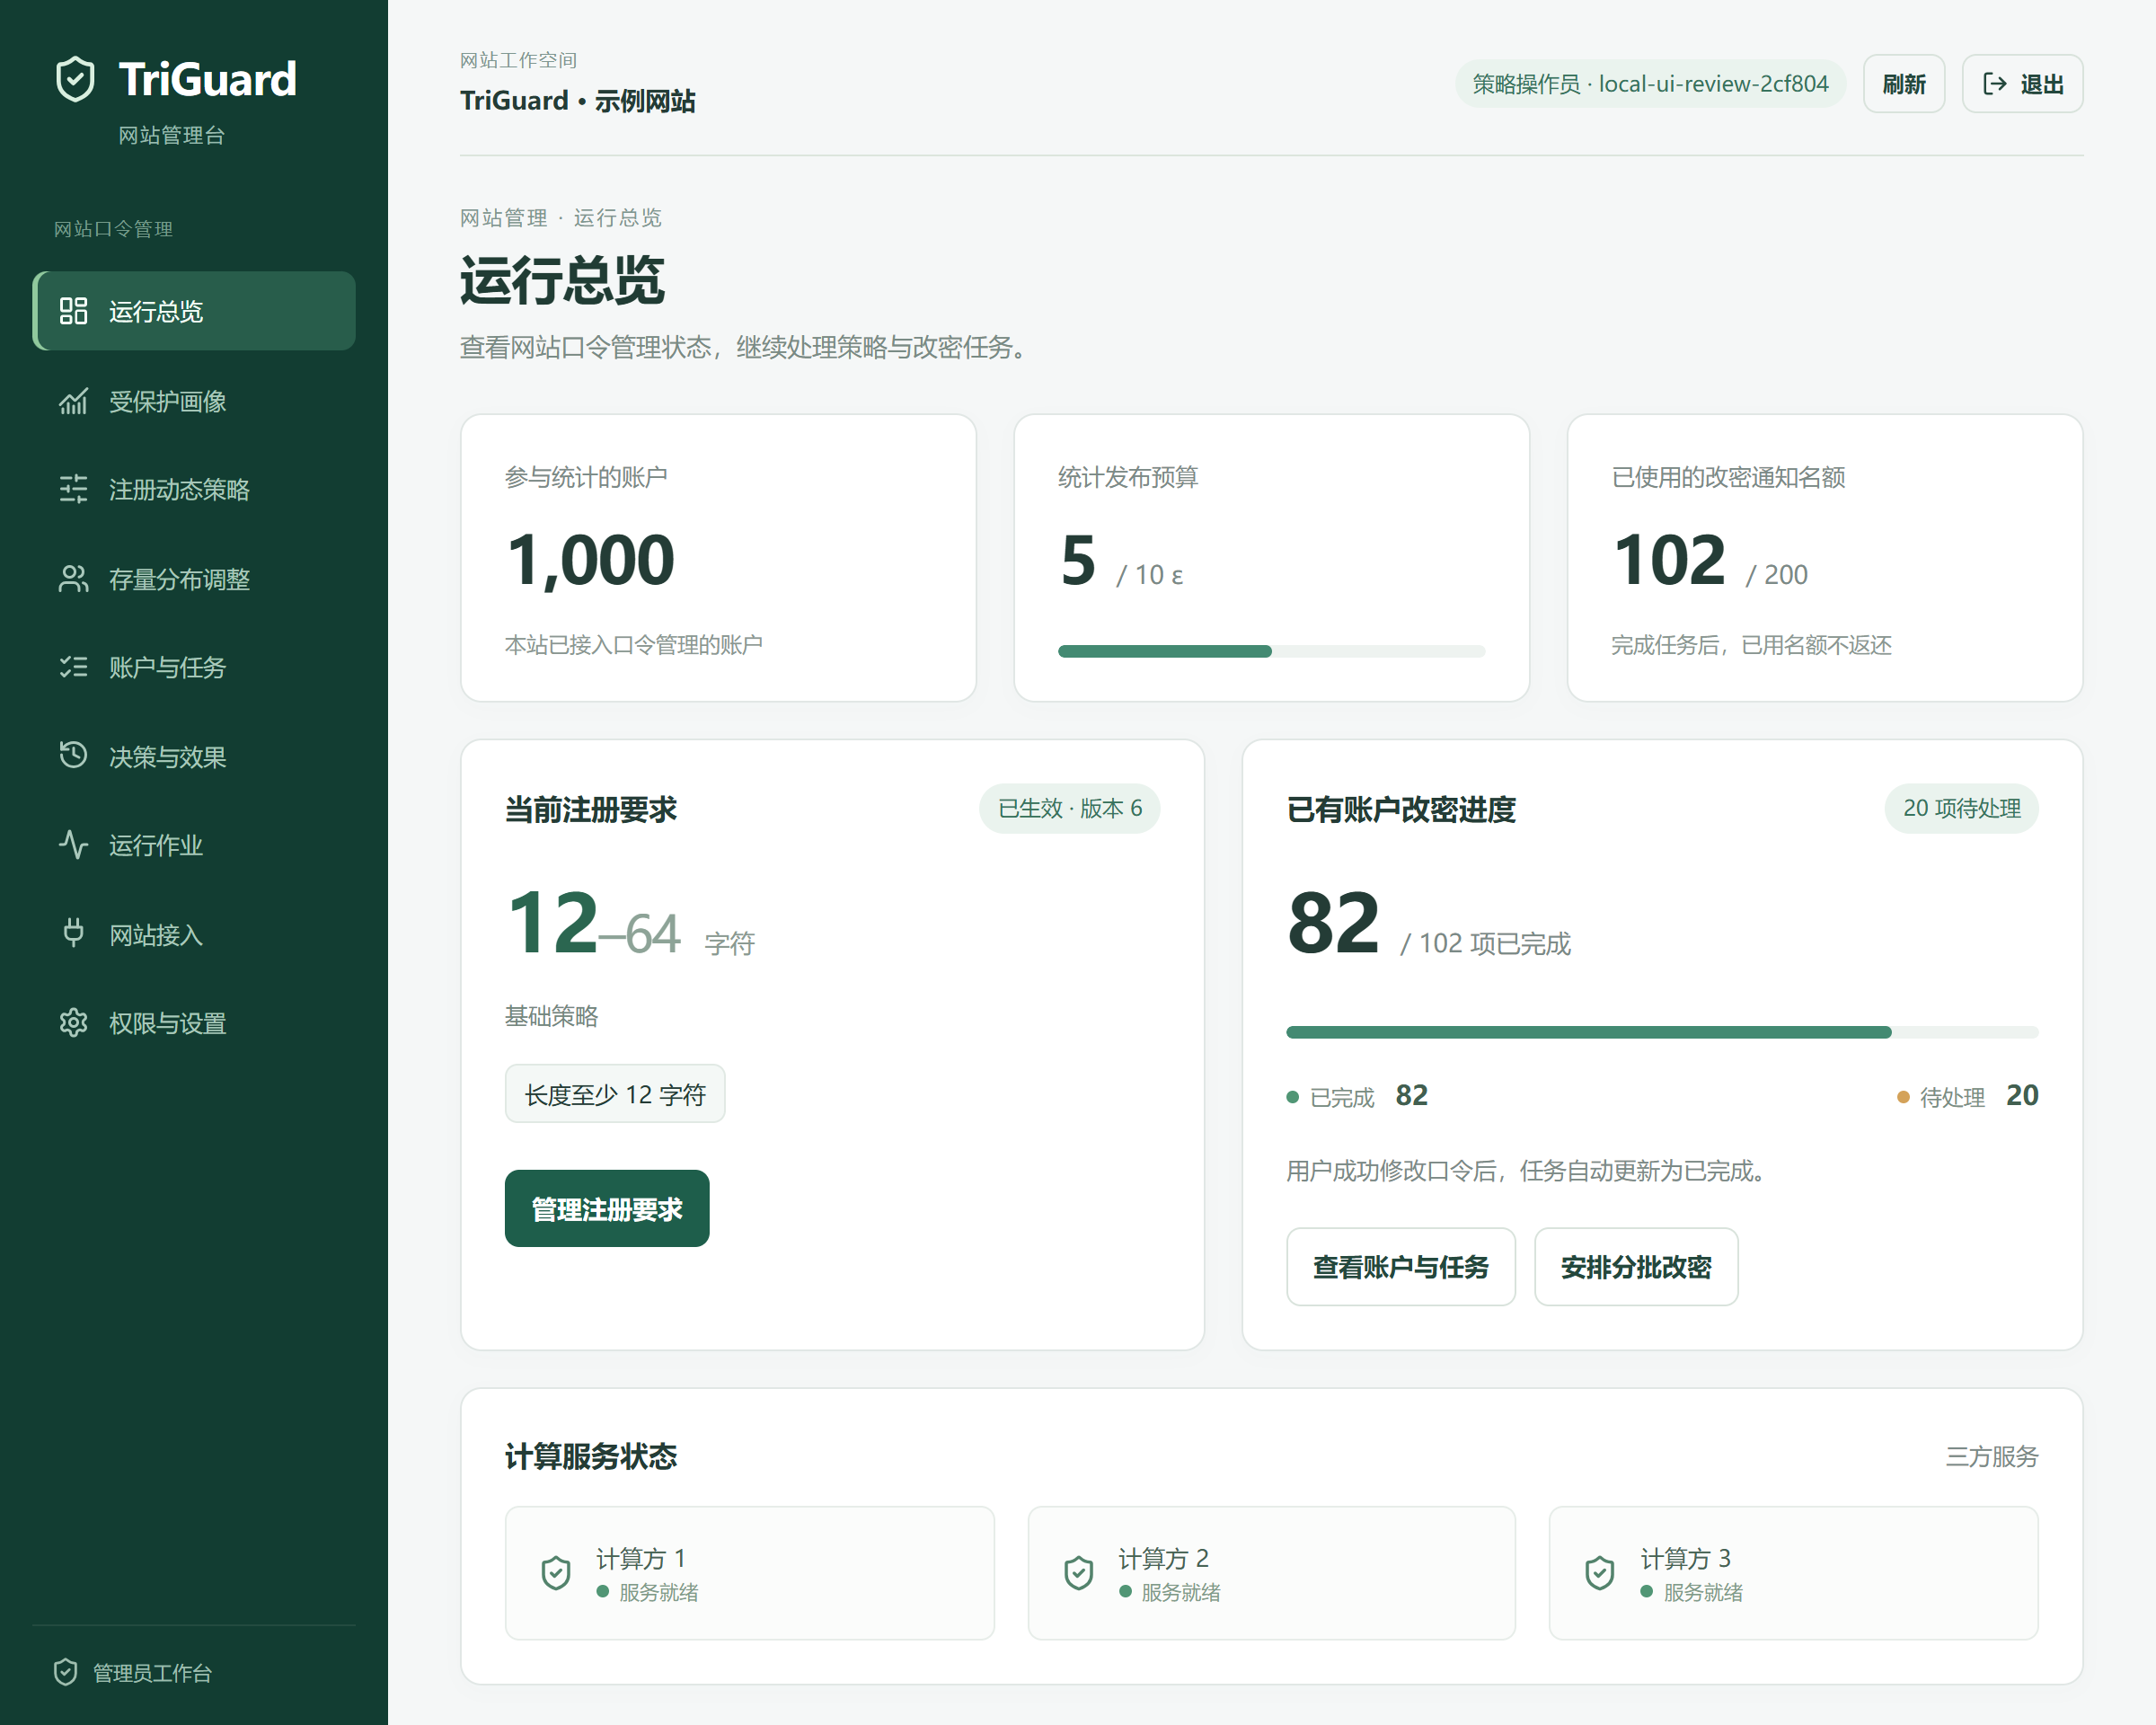
\includegraphics[width=\linewidth,height=0.64\textheight,keepaspectratio]{tool-admin-overview-2-2.png}
\caption{\quad 管理员网站工作台：全站统计预算、当前生效要求与累计改密进度}
\label{fig:tool-admin-overview}
\end{figure}

\subsubsection{管理员查看受保护的口令统计}\label{sec:implementation-profile}

管理员进入“受保护画像”，查看各类字符结构的估计人数，以及每类结构内重复最多的完整口令频次。结构用字母、数字和符号的组成方式表示，例如L8表示8位小写字母。完整口令只以所在结构和匿名名次呈现，页面不显示该名次对应的真实字符串；账户列表也不提供个人口令结构。图\ref{fig:tool-admin-profile}中，左侧显示热门结构的估计人数，右侧显示结构内匿名频次；管理员据此判断集中使用的形式及其重复程度，无需下载用户口令名单。

统计由三方共同计算并加噪发布，页面记录快照编号、统计人数和本次隐私预算。管理员可重复读取同一快照；用户注册或改密后，当前秘密状态会更新，已发布快照仍保留原值。只有按预算发布新快照，页面才显示新的分布。结构人数、匿名频次和规则违反人数都是含噪估计，适合为策略选择提供依据，不能当作逐账户的精确明细。

\begin{figure}[H]
\centering
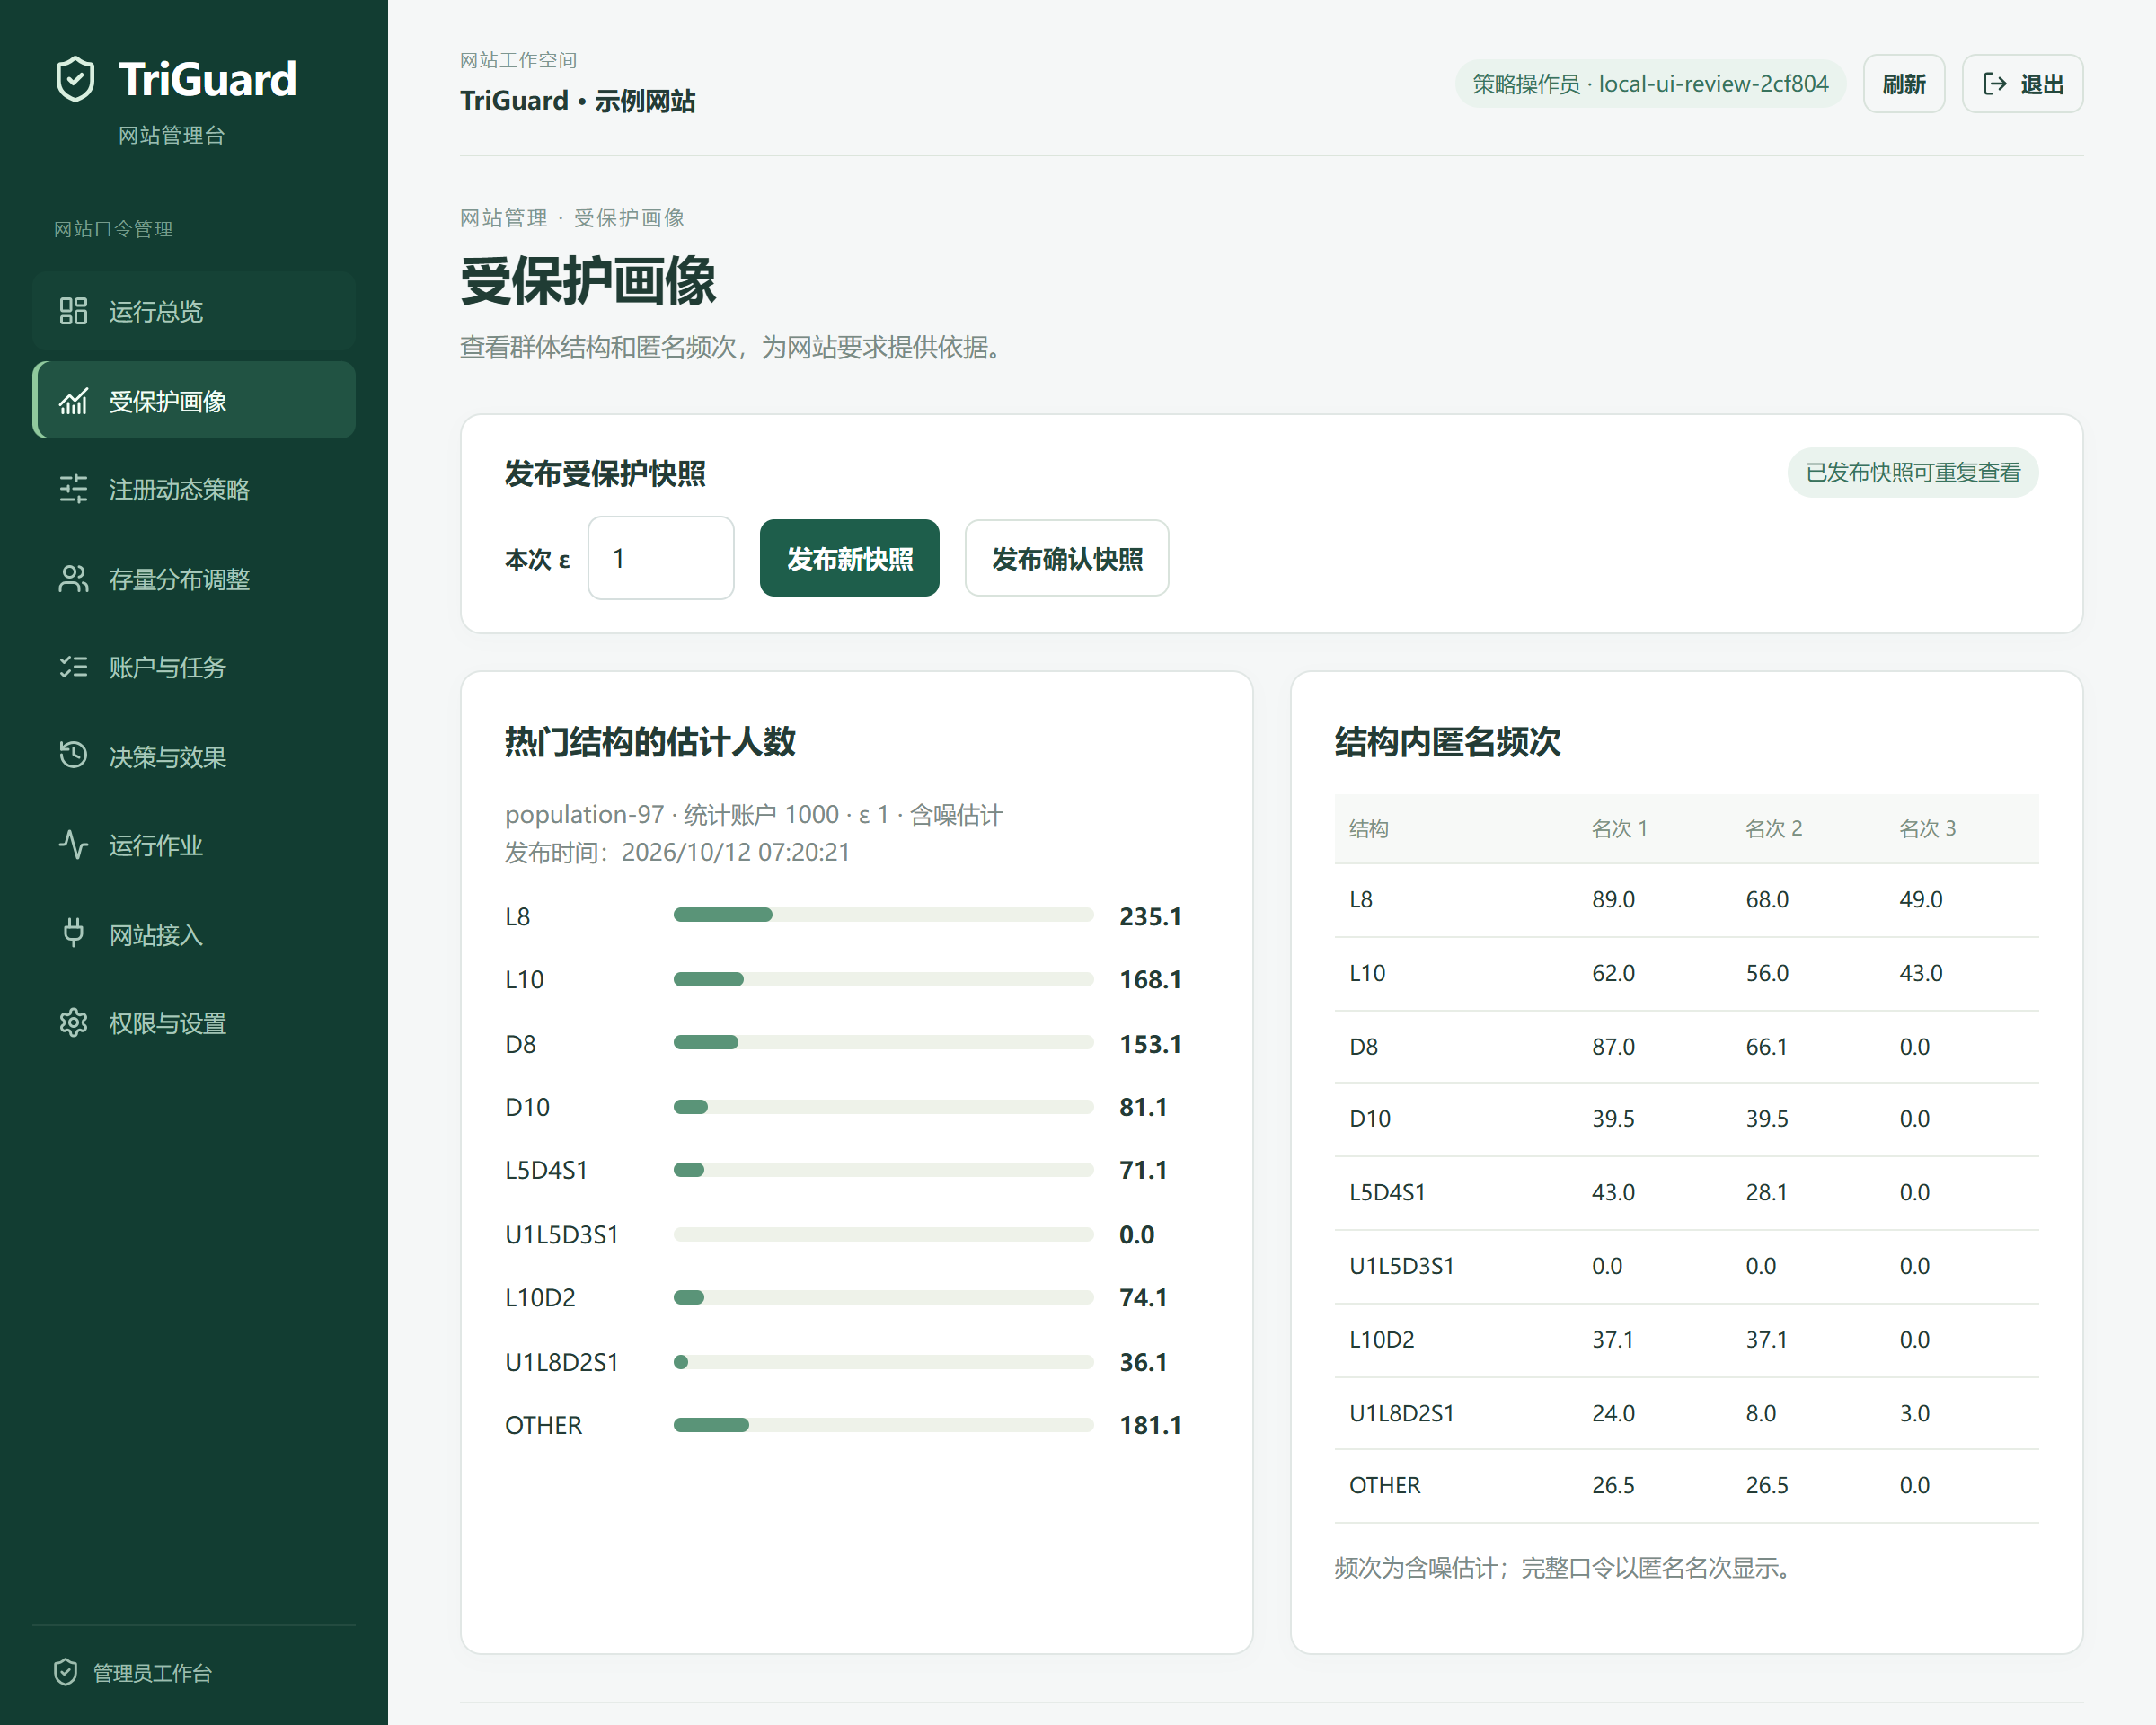
\includegraphics[width=\linewidth,height=0.64\textheight,keepaspectratio]{tool-admin-profile-2-2.png}
\caption{\quad 管理员受保护统计：群体结构人数与匿名热门口令频次}
\label{fig:tool-admin-profile}
\end{figure}

在线统计固定为8个结构加OTHER，每类保留前3名。另发布18项规则的违反人数估计：17项固定规则各最多变化1人，热门口令前三名覆盖人数最多变化2人，敏感度上界为19。每次发布预算的80\%用于核心统计、20\%用于违反人数，分别按4和19配置离散拉普拉斯噪声。预算先保存，发布失败或结果未知时保留已用额度，达到累计上限后停止发布。


\subsubsection{管理员制定注册与改密要求}\label{sec:implementation-registration}

“注册动态策略”将基础要求和依赖当前分布的附加限制放在同一入口。基础要求可设置策略名称、最短与最长长度，并从18类规则中组合长度、字符组成、重复与序列、常见与热门口令等要求。界面按这四类组织规则，管理员可同时查看所选条件。管理员勾选确认后提交，后台经三方执行和结果核验形成新的策略版本，再由用户插件读取。新要求作用于后续注册和改密，旧账户登录仍只验证当前凭据，避免要求更新后用户无法进入账户。

图\ref{fig:tool-registration-rules}展示基础要求的编辑状态：长度设置为12至64字符，额外勾选“至少一个数字或符号”，但确认框尚未勾选，应用按钮不可用。因此，这张图保留网站导航、规则分组和提交确认区，说明管理员如何组成待提交要求；已经生效的要求仍以运行总览和用户插件显示的版本为准。把编辑与生效分开，能够减少误操作，也便于核对用户实际收到的要求。

对于集中使用的问题，管理员还可以绑定一个统计快照，选择要限制的字符结构，并从其他结构中选择热门完整口令的匿名位置。当前选择阈值为结构人数估计至少20、完整口令频次估计至少2。例如限制某类纯数字结构后，该结构中的热点便不再重复占用完整口令名额。三方保存匿名位置与秘密字符串的对应关系，注册或改密时执行真实比较。历史版本支持回退，但回退只改变后续要求，不恢复用户已修改的口令。当前工具已接入完整口令与整类结构联合限制。完整分布评价、双模型训练、用户重选预览和自动确认在离线实验中运行；缺少本站用户重选与成本依据时，自动候选保持现有策略，管理员手动设置与自动选择分别记录。

\begin{figure}[H]
\centering
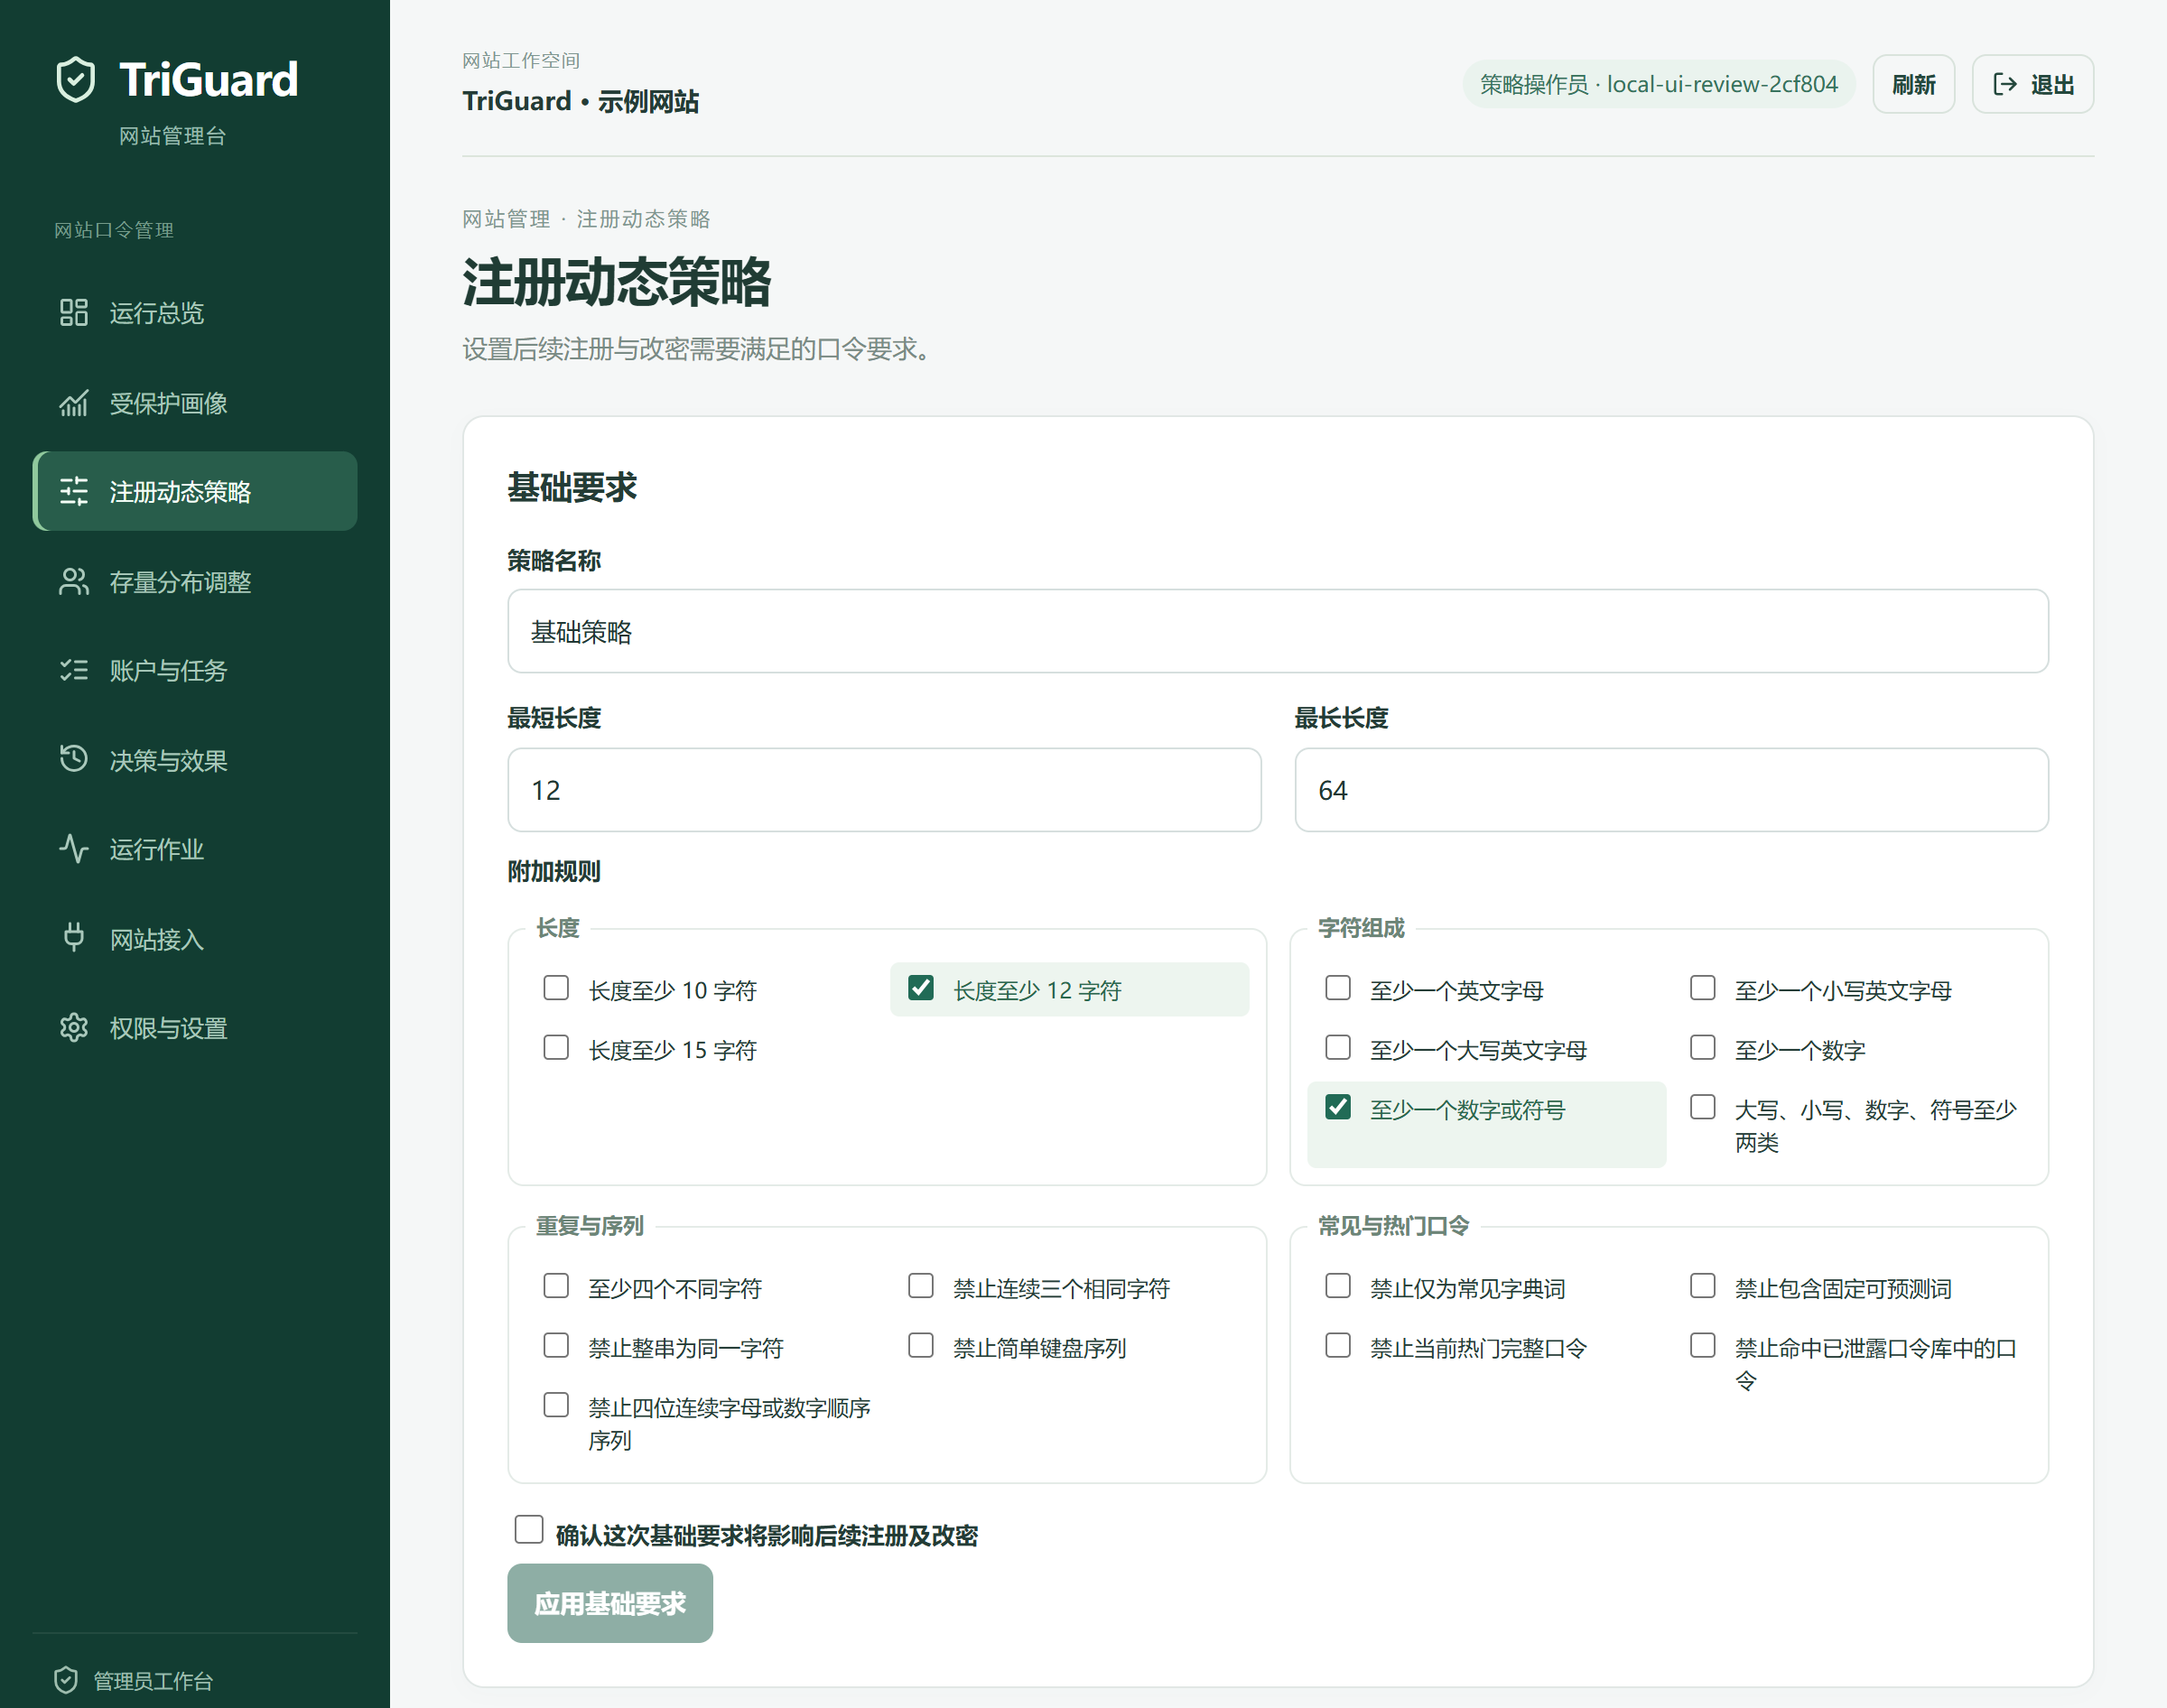
\includegraphics[width=\linewidth,height=0.64\textheight,keepaspectratio]{tool-registration-rules-2-2.png}
\caption{\quad 注册基础要求的编辑界面}
\label{fig:tool-registration-rules}
\end{figure}

\subsubsection{管理员安排已有账户分批改密}\label{sec:implementation-intervention}

“存量分布调整”将已有账户的改密安排与新注册要求分开。管理员先查看不同规则的违反人数估计，再设置本轮与累计分配上限，选择本次任务要求并确认。计算方在秘密状态下判断账户是否违反所选要求，跳过停用账户和已有待处理任务的账户，在剩余额度内分配任务。管理员获得必要的分配结果，用户只在本人任务页看到自己的要求。

图\ref{fig:tool-intervention-rules}中的勾选示例为“长度至少10字符”和“至少一个数字”，同样处于尚未确认的状态。多条规则会共同约束新口令，且任务要求要与当前网站要求同时满足；例如本站已要求至少12字符时，任务中的10字符门槛不会将其放宽。这张图展示通知名额、规则组合与提交确认三个操作环节；它是编辑示例，不对应千用户流程中实际采用的“至少15字符”任务。

本机展示配置将单轮上限设为20人、累计上限设为200人，便于分批通知和观察待处理状态。任务完成不返还已经使用的通知名额，发出任务也不计为完成。下一轮可结合新的画像和实际处理进度重新选择要求。当前在线工具按18类规则组织任务，承接2.1.1的分批调整与人数控制思路；离线算法中的双模型攻击评价和收益预测仍在相应实验中说明，不能仅由任务完成数量推出攻击风险下降。

\begin{figure}[H]
\centering
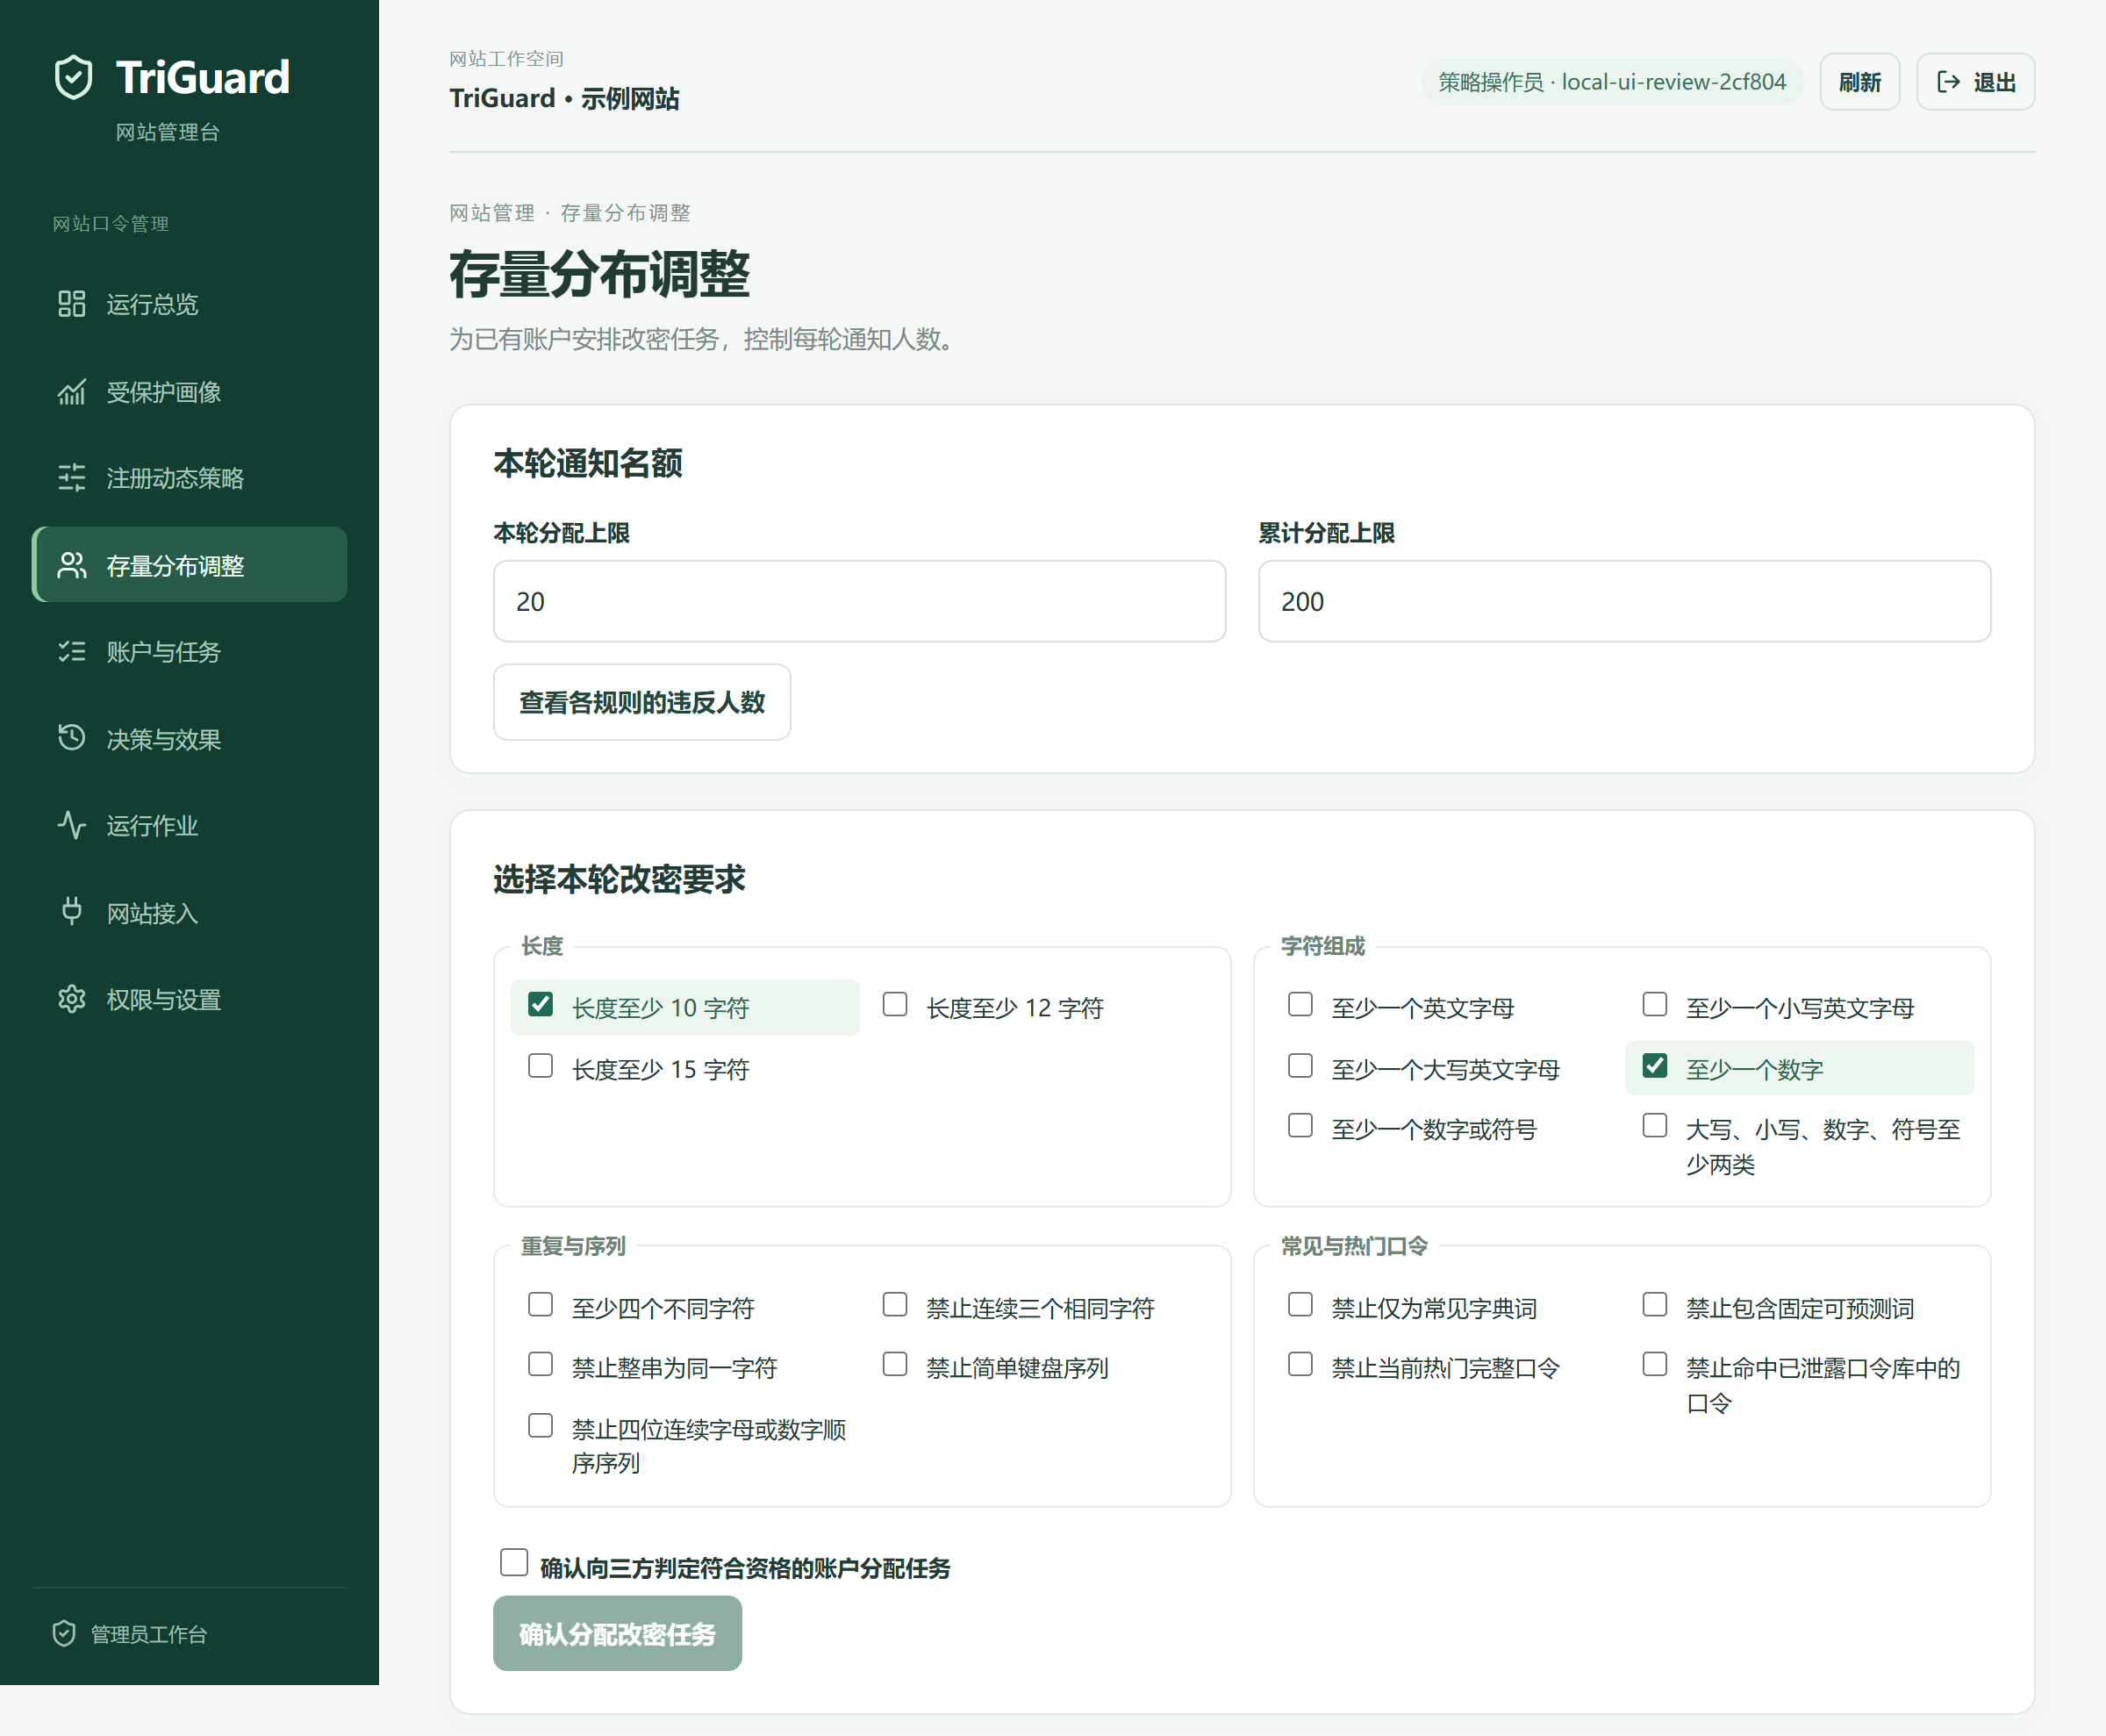
\includegraphics[width=\linewidth,height=0.64\textheight,keepaspectratio]{tool-intervention-rules-2-2.png}
\caption{\quad 已有账户改密任务的规则组合界面}
\label{fig:tool-intervention-rules}
\end{figure}

\subsubsection{用户选取口令与获得检查反馈}\label{sec:implementation-assistant}

用户在独立浏览器插件的“口令助手”中输入候选口令。顶部标明“浏览器扩展”，导航围绕口令助手、我的任务、我的账户和站点连接组织；右侧显示本站当前长度要求和策略版本，输入框以掩码显示内容。“本地检查”无需上传口令，先检查长度、可打印字符、公开弱口令参照、重复字符及常见键盘或连续序列，并用短句说明需要修改什么。口令输入保留在当前页面内存中，不写入浏览器持久存储。当前协议支持8至64个可打印ASCII字符，实际最低长度还要符合本站策略。

图\ref{fig:tool-user-feedback}展示本地拒绝反馈。页面显示9字符的掩码输入，右侧提示长度不足、口令较常见以及存在键盘或连续序列；用户可以据此增加长度、调整组合，再次检查。反馈提供具体修改方向，降低只看到“口令不合格”时的困惑；本地检查还包含公开的建议性筛查，因此出现某条提示不等于网站已将该条设为强制规则。

用户随后可点击“检查本站要求”。插件将同一口令转换为三份随机份额，分别直接发送给三个计算方；三方检查基础要求、被限制结构和隐藏热点，返回合并的通过或拒绝结果。网站业务服务不接收明文口令，也不汇集三份输入。这个入口补足了本地检查无法判断的隐藏限制：本地提示帮助用户修改，私密检查落实本站完整要求，但不会告知命中了哪一个秘密热点。

\begin{figure}[H]
\centering
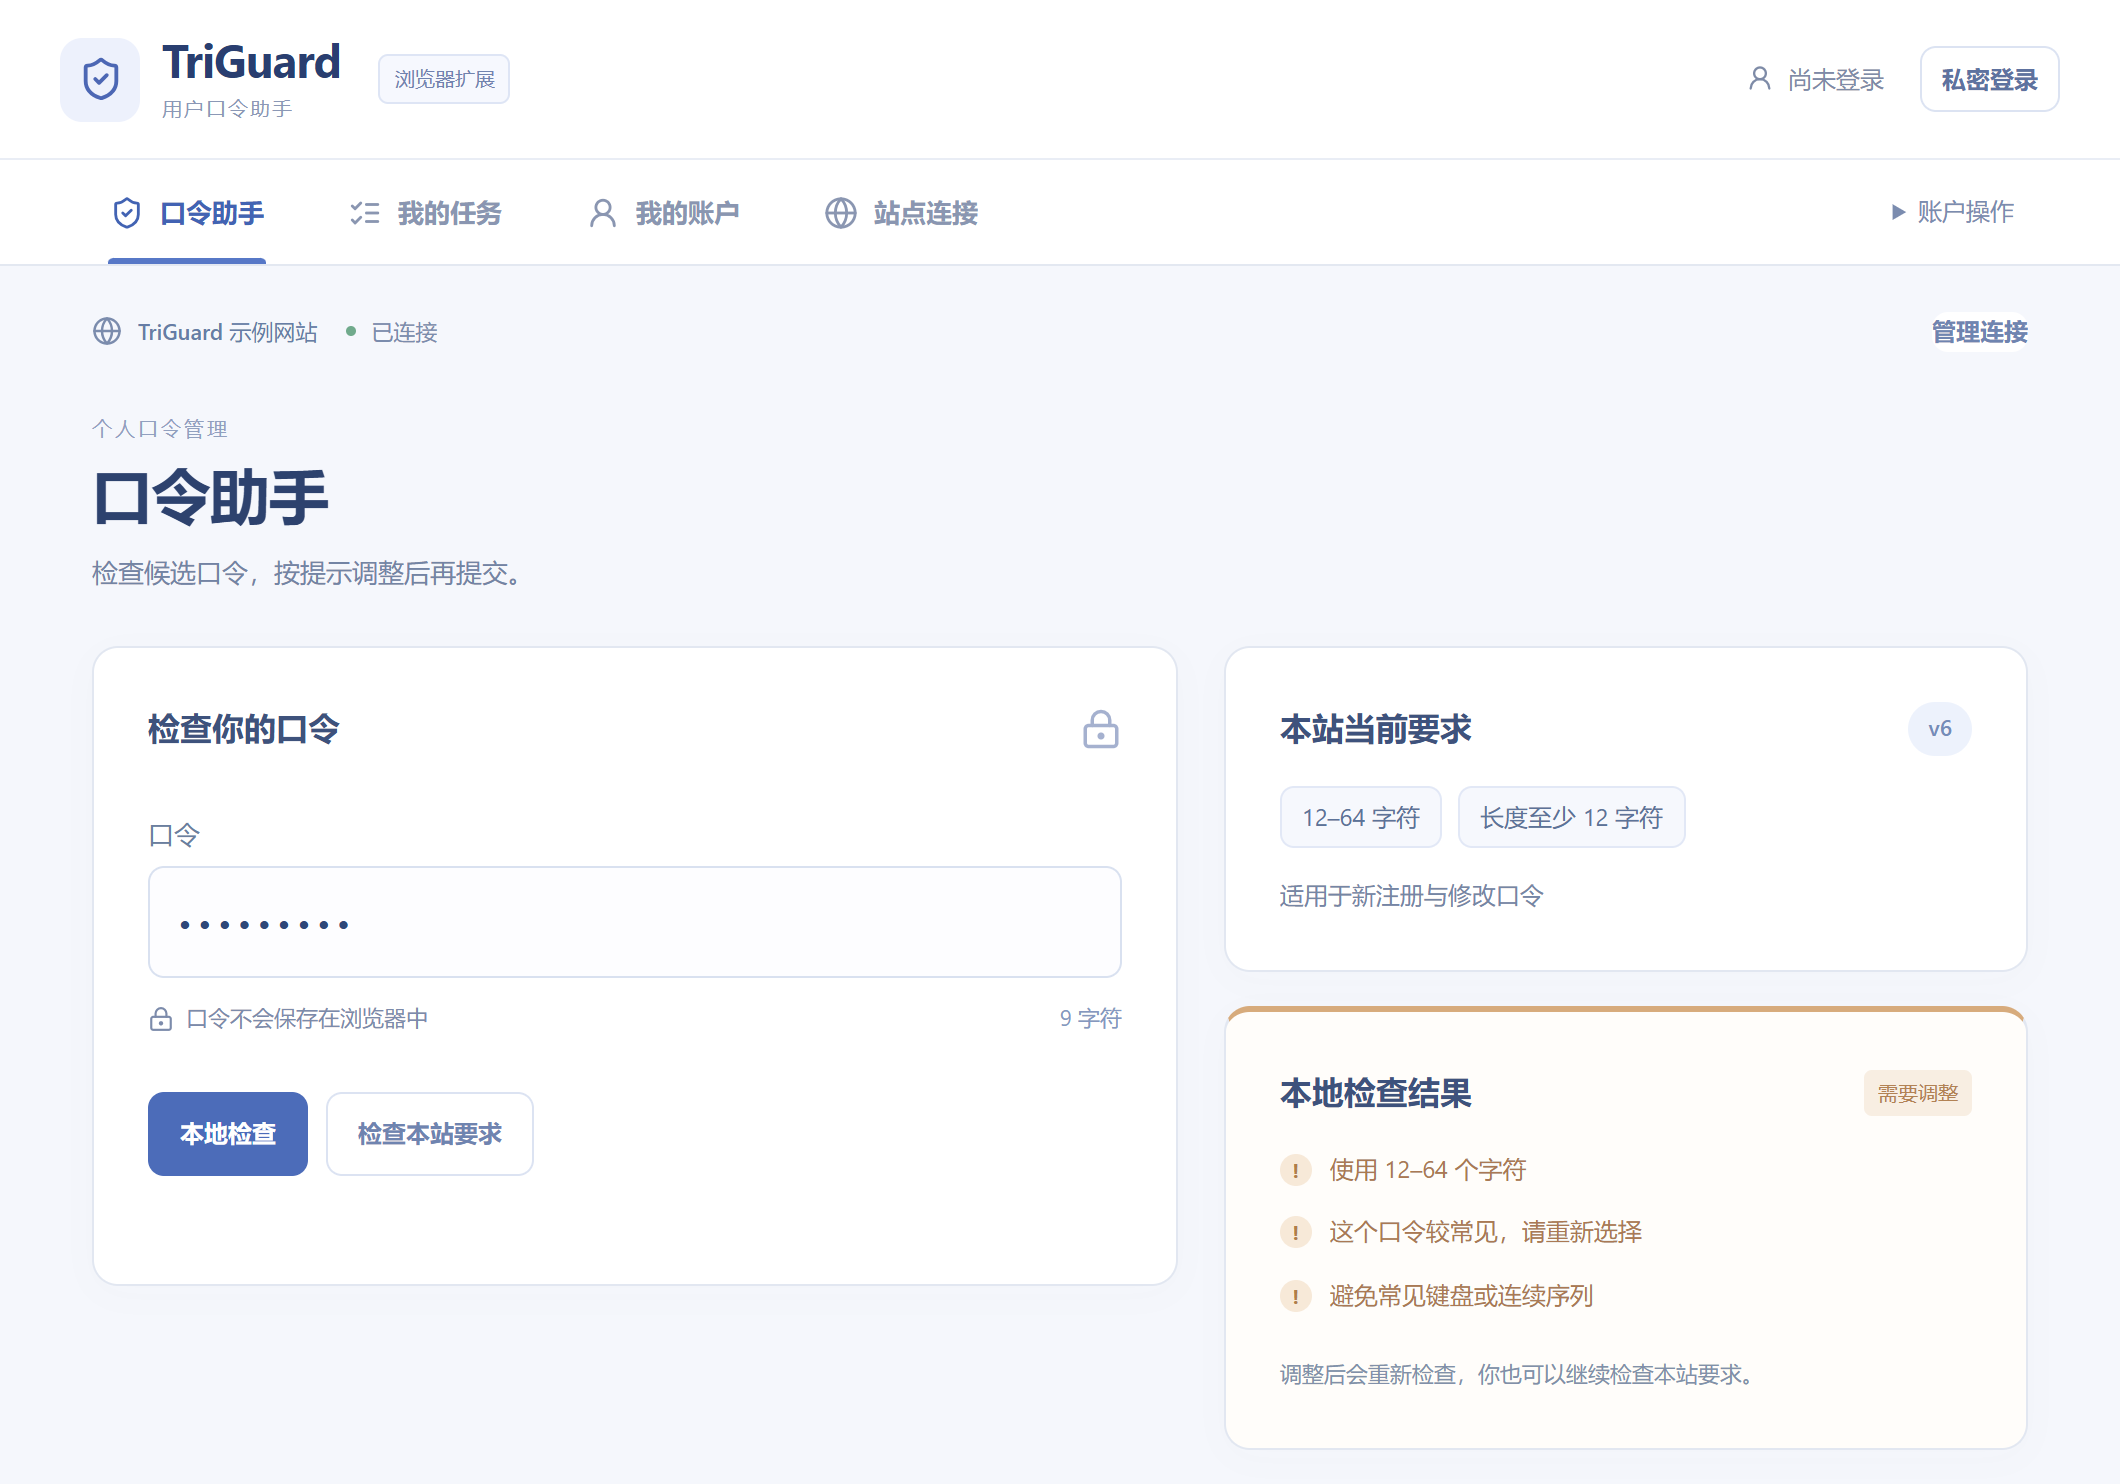
\includegraphics[width=0.99\linewidth,height=0.72\textheight,keepaspectratio]{tool-user-feedback-2-2.png}
\caption{\quad 用户浏览器插件：本人候选口令的本地反馈与本站当前要求}
\label{fig:tool-user-feedback}
\end{figure}

\subsubsection{用户账户操作与改密任务反馈}\label{sec:implementation-tasks}

插件同时提供注册、私密登录、历史账户接入、修改口令、本人任务和恢复账户入口。账户注册增加统计贡献，改密或恢复替换旧贡献，注销撤销贡献。注册通过规则检查后建立秘密凭据；登录在秘密状态下比较输入与当前凭据；改密先验证旧口令，再检查新口令是否同时满足本站要求和本人任务。历史账户接入需要原网站授权，不能覆盖已经接入的账户。恢复时使用用户保管的恢复凭证证明授权，成功后更换凭证，管理员没有直接查看或代设用户明文口令的入口。

已有账户收到任务后，在“我的任务”查看待处理状态与具体要求，再进入改密页填写旧口令、新口令及确认值。只有改密实际成功，后台才替换旧凭据和旧统计贡献，并将任务记为完成；用户未响应、退出或新口令被拒绝时，任务仍待处理。管理员在“账户与任务”中按账户标识查看版本和状态，在总览查看累计进度；图\ref{fig:tool-task-contrast}展示同一合成账户的两端任务视图：管理员按账户标识筛选后看到凭据版本、待处理状态和启停操作；用户插件只显示本人任务，并给出“长度至少15字符”的具体要求及改密入口。用户同时仍需满足本站现行要求。两端据此追踪同一项任务，各自取得权限允许的内容。操作绑定请求编号、账户版本和策略版本；三方保存待提交状态，再签署决定并更新凭据、贡献与任务。失败、预检查和重复请求保留原统计，中断后按原请求恢复。

\begin{figure}[H]
\centering
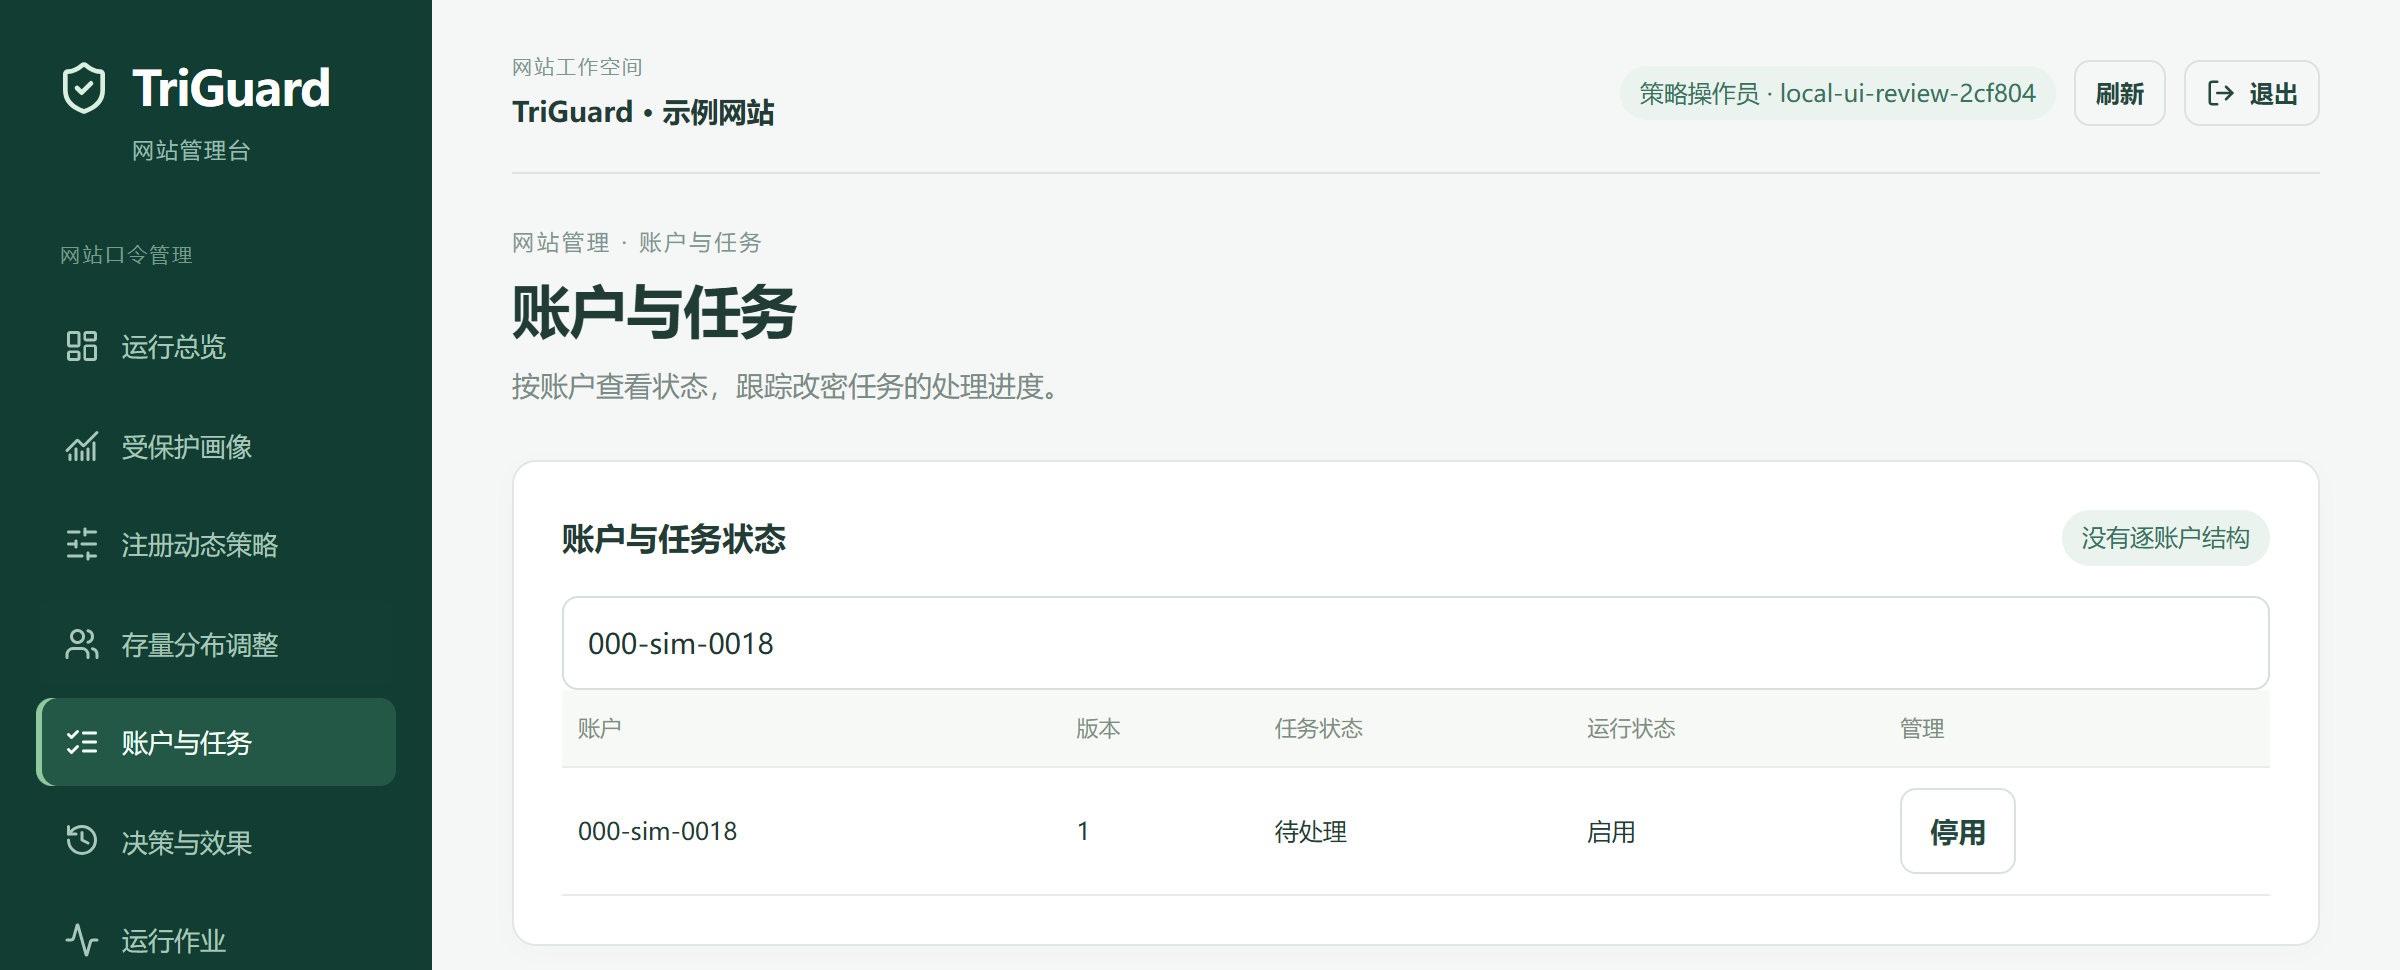
\includegraphics[width=\linewidth]{tool-admin-task-2-2.png}
\par\smallskip
{\small （a）管理员网站：按账户跟踪任务状态}
\par\medskip
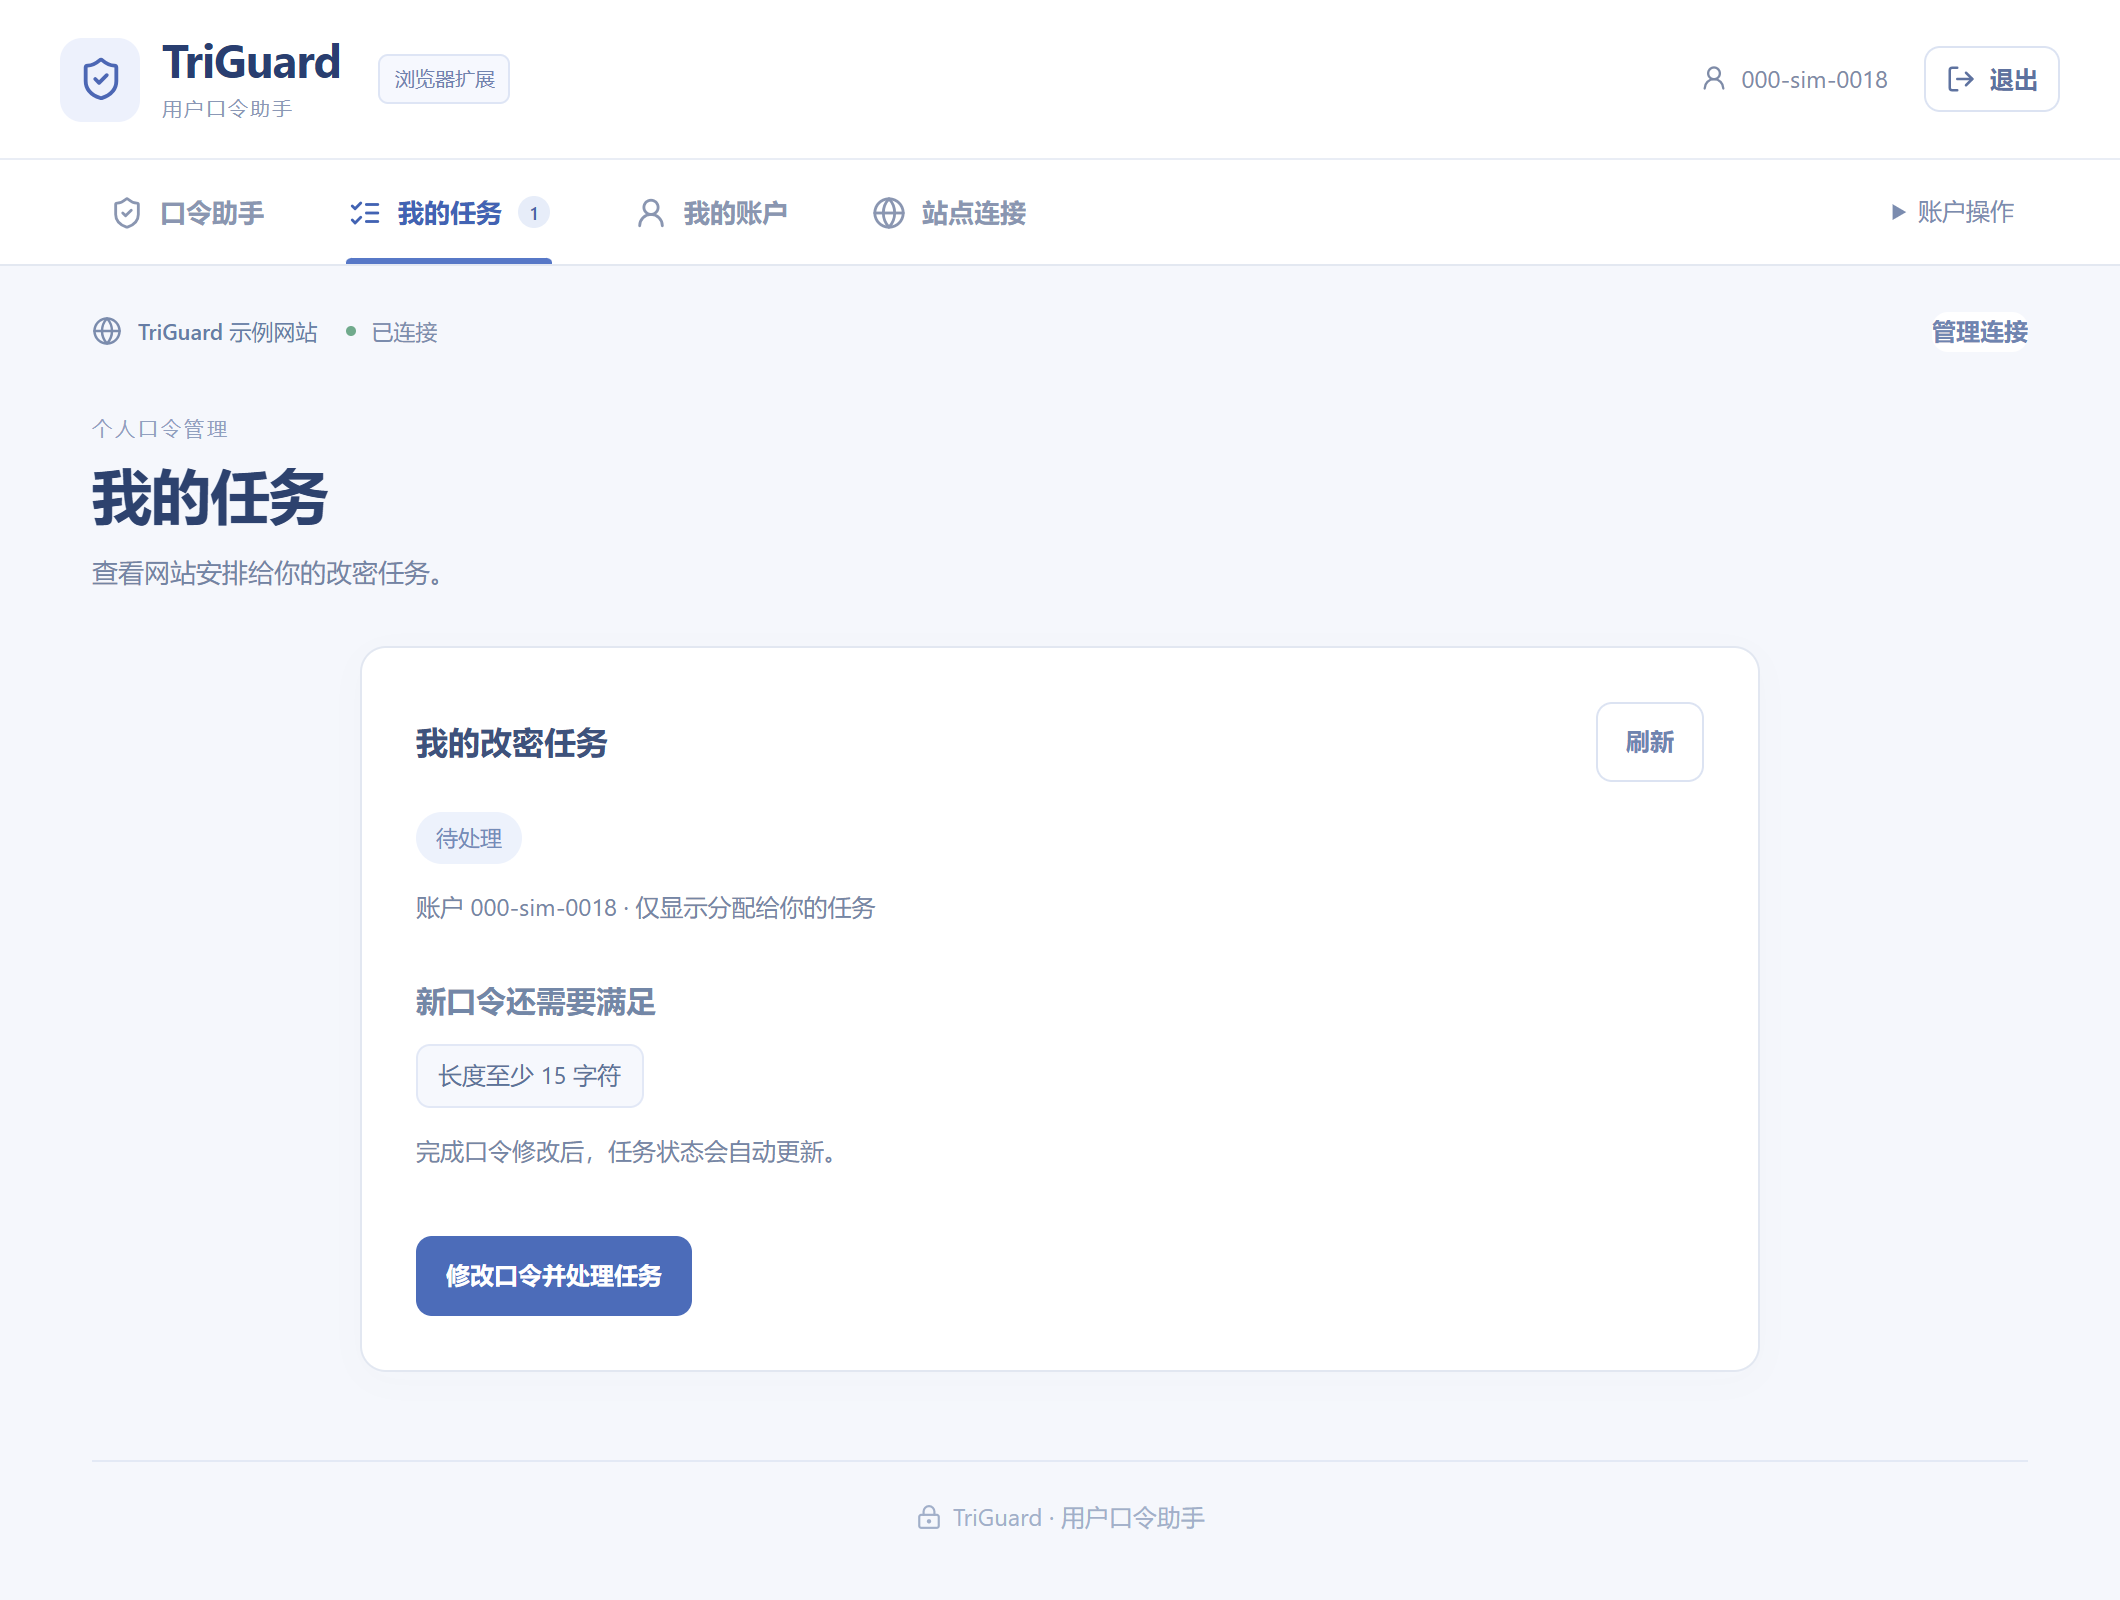
\includegraphics[width=0.90\linewidth]{tool-user-task-2-2.png}
\par\smallskip
{\small （b）用户插件：查看本人要求并进入口令修改}
\caption{\quad 同一账户的两端任务视图：网站管理与本人操作的分工}
\label{fig:tool-task-contrast}
\end{figure}

\subsubsection{网站接入与运行管理}\label{sec:implementation-operations}

合作网站通过一次性挑战和三方认证证明接入系统。网站先生成随机挑战，用户在插件内使用该挑战完成私密认证，再把证明交给网站；网站核对三方签名、站点、挑战和账户版本后建立会话。作品提供了独立接入样例，当前需要手工传递挑战与证明。该网页用于说明合作网站如何使用认证结果，用户的口令输入和操作仍在浏览器插件中完成。

图\ref{fig:tool-site-challenge}展示合作网站接入页的认证完成状态。页面按“获取一次性挑战—在插件内完成认证—网站验证并建立会话”三个步骤组织；左侧保留本次随机挑战及插件操作指引，右侧显示三方回执已通过核验、登录账户和已建立的网站会话。验证成功后，挑战标记为“已使用”，相同挑战与证明不能再次建立会话。图中账户为本地合成测试账户，用于说明网站接入流程；该页面不提供口令输入框。

\begin{figure}[H]
\centering
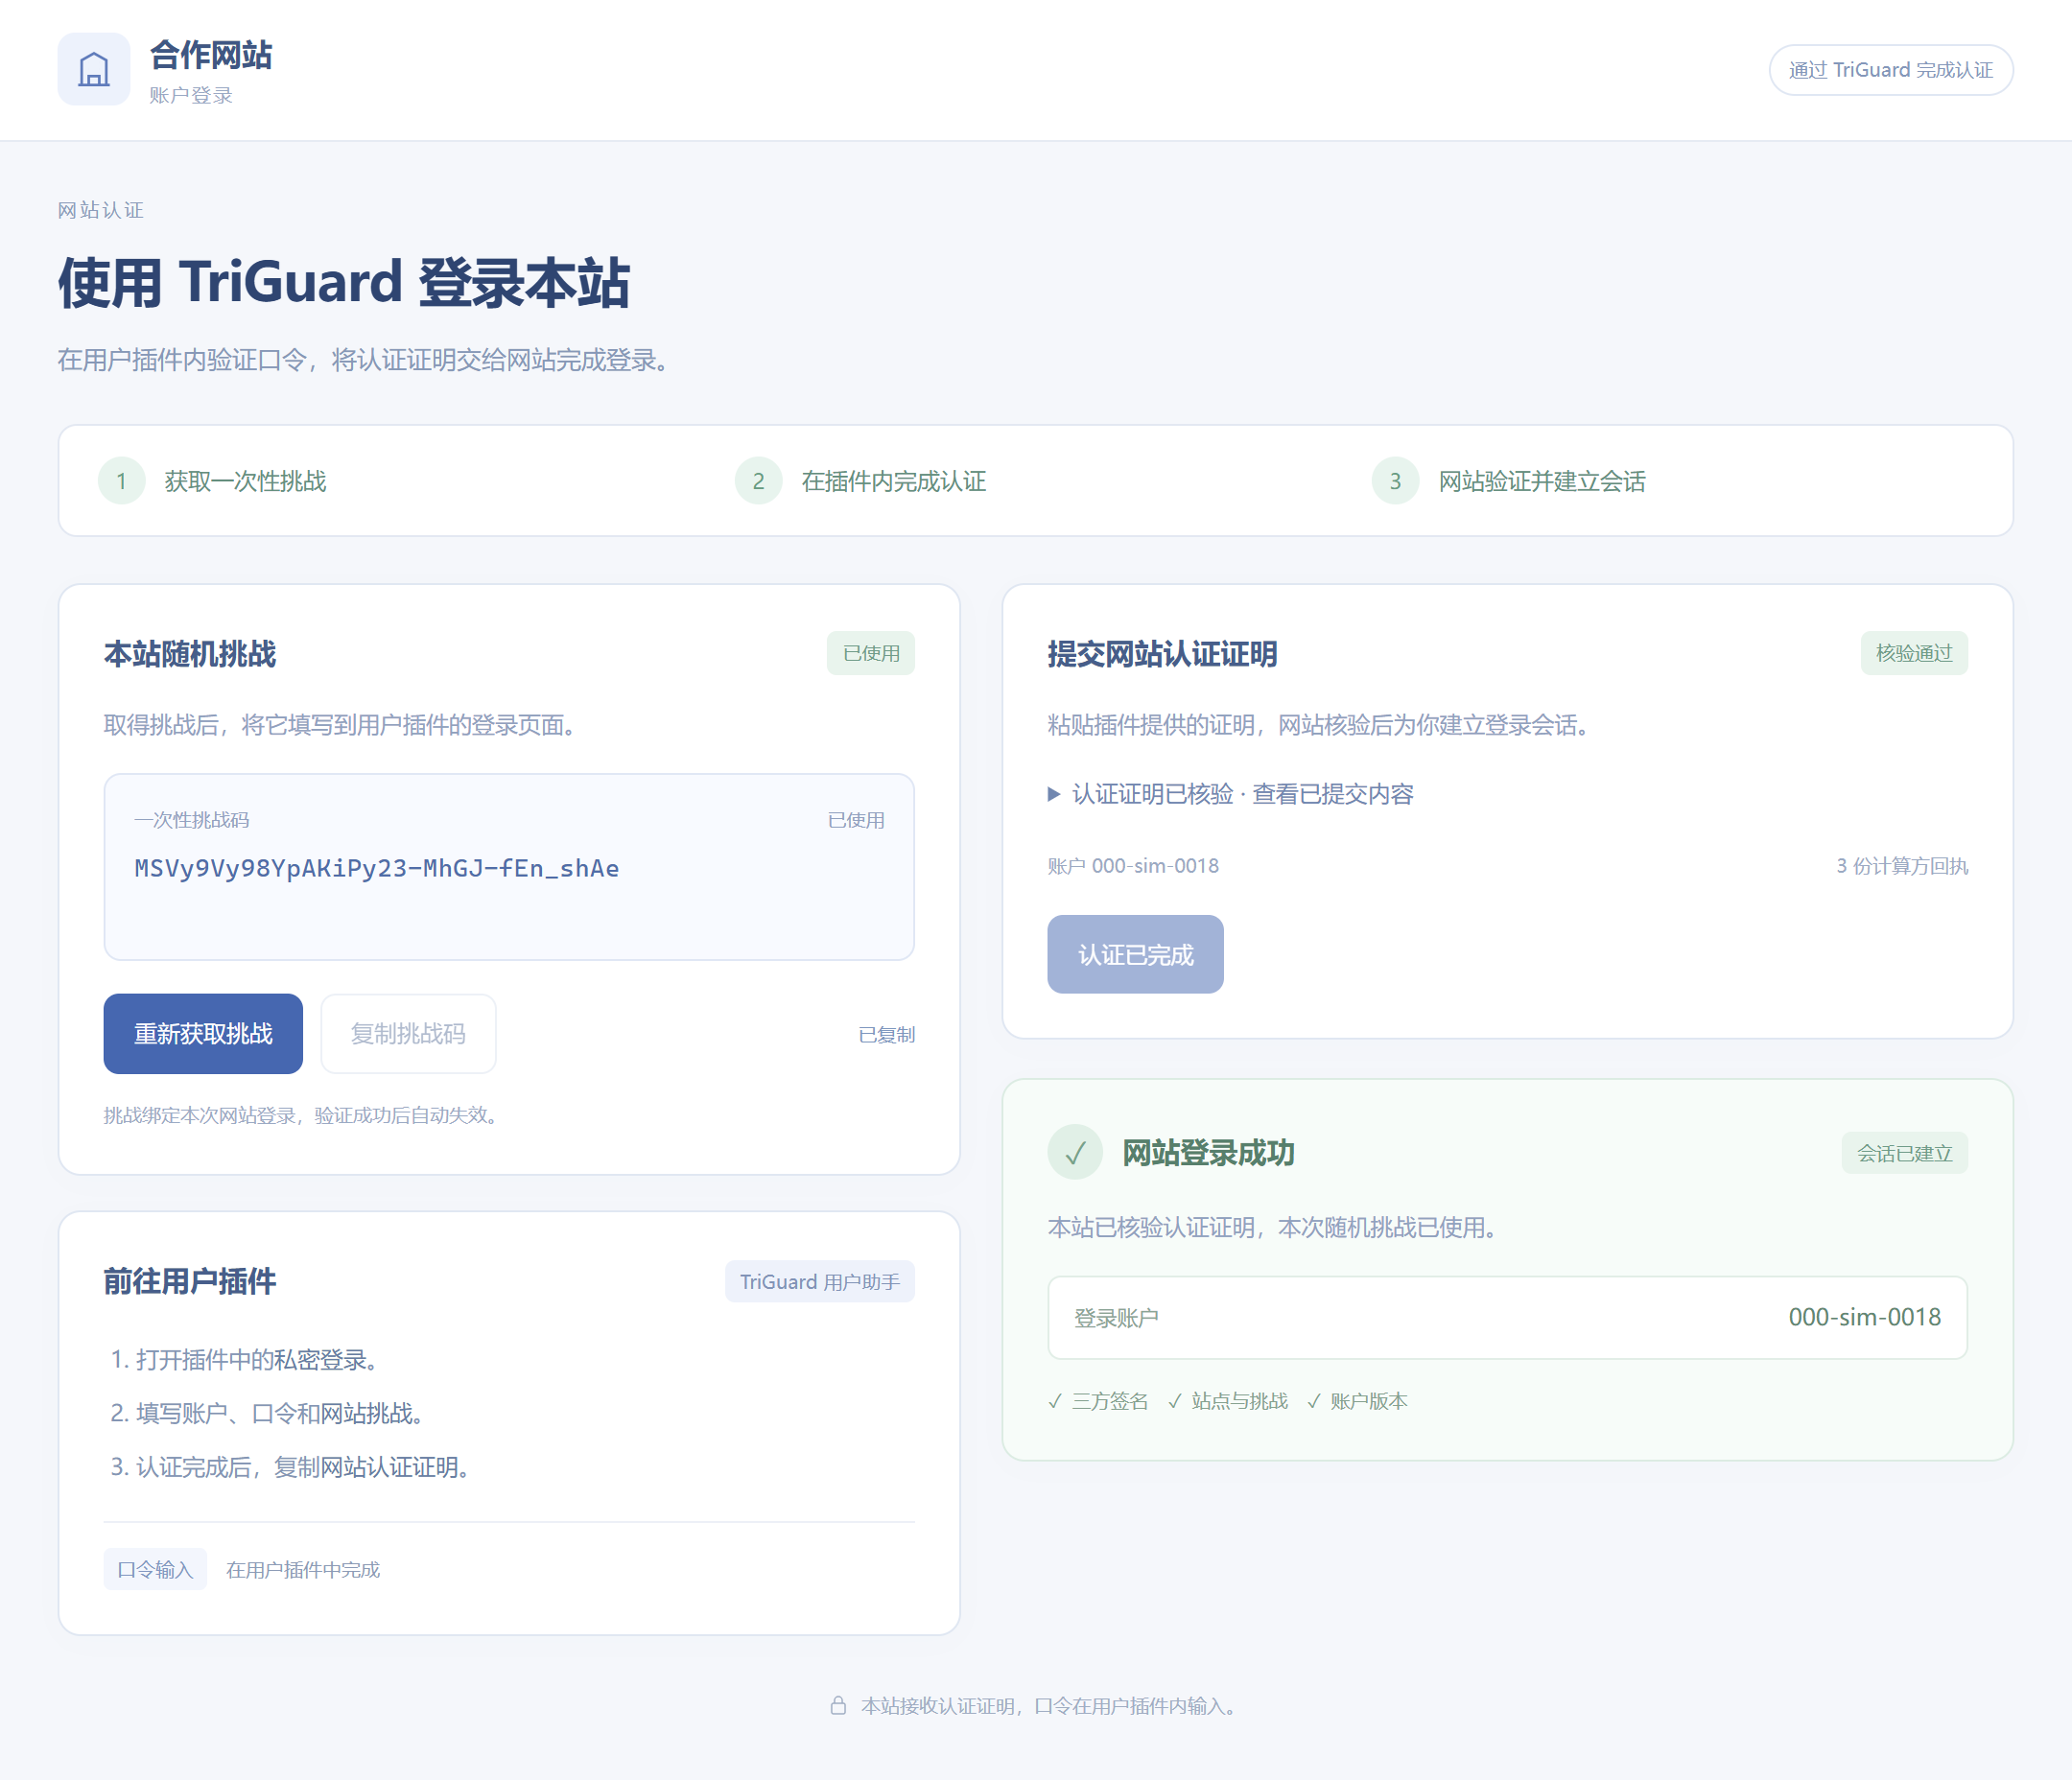
\includegraphics[width=\linewidth,height=0.64\textheight,keepaspectratio]{tool-site-challenge-2-2.png}
\caption{\quad 合作网站的随机挑战认证页面：插件证明核验通过后建立本站会话}
\label{fig:tool-site-challenge}
\end{figure}

管理员使用通行密钥登录，后端按负责人、操作员和只读审计员区分权限。用户与管理员的会话和访问入口分开，策略、本人任务及受保护汇总经后端按权限传递。账户身份、检查结果和任务状态按业务权限管理，统计发布按隐私预算管理。耗时统计和任务分配放入后台作业，页面可查看状态；操作中断或结果未知时，继续查询原请求，核对三方结果后再确认成功。上述设计把选取提示、策略执行、任务跟踪与网站认证连在一起，为网站提供持续管理口令的工具，也为用户提供独立完成口令操作的入口。


\clearpage
\section{作品测试与分析}\label{ux7b2cux4e09ux7ae0-ux4f5cux54c1ux6d4bux8bd5ux4e0eux5206ux6790}

本章分别验证已有账户调整的分布与攻击效果、动态注册相对固定名单的改善，以及秘密传输和匿名统计的隐私保护与使用效果。

\subsection{已有口令集分布动态调整方案验证}\label{sec:validation-existing}

本节通过两个实验验证第\ref{sec:design-existing}节的方法。实验一比较原始基线、8字符基础策略、随机策略、固定策略和动态策略：动态与随机策略的对比检验按分布选择修改对象的作用，动态与固定策略的对比检验依据反馈重新决策的作用。实验二与HTPG方法比较，评价完整口令分布及抗猜测效果。

\subsubsection{实验设置}\label{sec:validation-existing-1}

实验以RockYou语料的每次出现代表一个模拟账户，种子为42。目标与开发记录各100,000条，出现位置互不重叠，字符串可重复；开发按60\%、20\%、20\%分为训练、调参与验证。随机、固定和动态三组从相同的8字符基础状态开始，共用18条候选规则、响应模拟与新口令检查。先运行动态组，再让两组匹配逐轮通知人数：均为6轮、每轮2,000人，后续共通知12,000人，同一账户在后续阶段至多通知一次，正式通知的账户全部成功改密。用户响应按局部修改、片段拼接和重新选取的60\%、25\%、15\%比例模拟；具体配置见附录B。

攻击评价采用PCFG与OMEN。F由开发训练记录建立，调整期间保持不变；A1用独立开发参考群体按相应策略修改后的口令重新训练，评价攻击者学习修改规律后的效果。原始基线未执行修改，训练数据保持不变，F与A1使用相同基线结果。每模型各猜测至100万次，联合最多200万次；重复猜测计入次数，账户重复命中计一次，命中率以全部100,000个目标账户为分母。分布采用第\ref{sec:design-existing}节的经验W1距离，数值越小，完整口令重复越少。

\subsubsection{实验一：基础策略与三种调整方式的对比}\label{sec:validation-existing-2}

原始基线保留初始口令，8字符基础策略只修改长度不足的口令，三种后续调整从该基础状态出发。随机策略每轮先在未接受后续通知的账户中随机抽取2,000人，再从共同规则池比较修改要求，选择预计分布改善最大的规则。动态策略与随机策略的对比用于验证按口令分布选择修改对象的作用。固定策略在共同起点按口令使用频次从高到低选择账户，提前确定各轮账户、修改要求和执行顺序；规划时保留起点分布并排除已分配账户，执行时沿用这份计划。动态策略与固定策略的对比用于验证根据逐轮执行反馈更新决策的作用。动态策略每轮依据修改后的实际分布重新选择对象与要求。五组的比较目的见表\ref{tab:comparison-methods}。

\begin{table}[H]
\centering
\caption{实验一的组别与比较目的}\label{tab:comparison-methods}
\small
\begin{tabularx}{\linewidth}{@{}lXX@{}}
\toprule
组别 & 处理方式 & 比较目的 \\
\midrule
原始基线 & 保留初始口令 & 给出调整前的分布与攻击结果 \\
8字符基础策略 & 修改长度不足8字符的口令 & 观察基础长度要求的改善 \\
随机策略 & 先随机选人，再比较修改要求 & 检验按分布选择对象的作用 \\
固定策略 & 按起点分布排好账户与要求 & 检验执行后反馈的作用 \\
动态策略 & 按每轮实际分布重新决策 & 评价对象选择与反馈更新的综合效果 \\
\bottomrule
\end{tabularx}
\end{table}

表\ref{tab:existing-final-distribution}汇总最终结果，图\ref{fig:validation-existing-2}展示不同猜测预算下的联合命中率。基础策略将W1从0.086247降至0.040946；后续动态组进一步降至0.000071，形成99,992个不同口令。动态组F、A1联合命中率分别为8.096\%、9.613\%，均为三个调整组中最低。

\begin{table}[H]
\centering
\caption{实验一的最终分布与联合命中率}\label{tab:existing-final-distribution}
\small
\begin{tabularx}{\linewidth}{@{}Xrrrr@{}}
\toprule
组别 & 不同口令数 & 经验W1 & F命中率 & A1命中率 \\
\midrule
原始基线 & 82,840 & 0.086247 & 36.900\% & 36.900\% \\
8字符基础策略 & 92,495 & 0.040946 & 16.627\% & 19.058\% \\
随机策略 & 93,741 & 0.034866 & 14.637\% & 16.472\% \\
固定策略 & 99,963 & 0.000284 & 8.632\% & 10.046\% \\
动态策略 & 99,992 & 0.000071 & 8.096\% & 9.613\% \\
\bottomrule
\end{tabularx}
\end{table}

\begin{figure}[H]
\centering
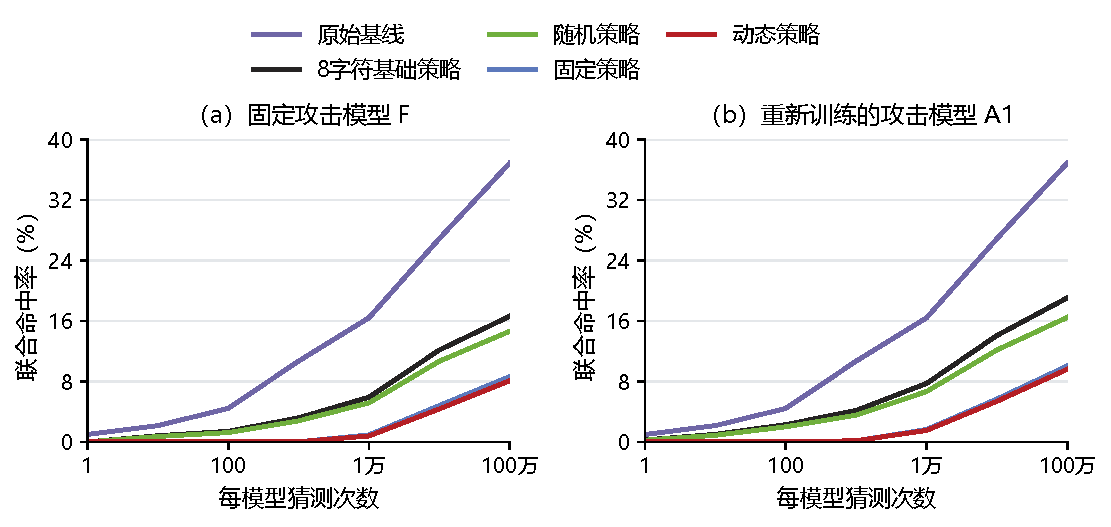
\includegraphics[width=\linewidth]{validation_3_1_internal.pdf}
\caption{\quad 实验一各组在F与A1下的联合命中率；横轴为每模型猜测次数，合计最多为其两倍}\label{fig:validation-existing-2}\label{fig:validation-existing-3}
\end{figure}

与随机策略相比，动态组F、A1联合命中率分别低6.541、6.859个百分点，表明依据口令分布选取修改对象能更有效地使用通知名额。与固定策略相比，分别低0.536、0.433个百分点，表明执行后的分布反馈带来了进一步改善。OMEN单模型中，动态组F、A1命中率分别为0.549\%、0.656\%，固定组为0.545\%、0.582\%；完整单模型结果、拟合距离与模型支持情况见附录\ref{app:existing-additional-results}。“按口令分布选择修改对象”和“根据逐轮执行反馈更新决策”都发挥了作用。

\subsubsection{动态调整的逐轮分布变化}\label{sec:validation-existing-3}

图\ref{fig:validation-existing-1}展示共同起点和六轮调整后的完整口令频次分布。动态组最高重复人数从258降至2，第6轮仅剩8个口令各被两个账户使用，最终形成99,992个不同口令，W1降至0.000071。

\begin{figure}[H]
\centering
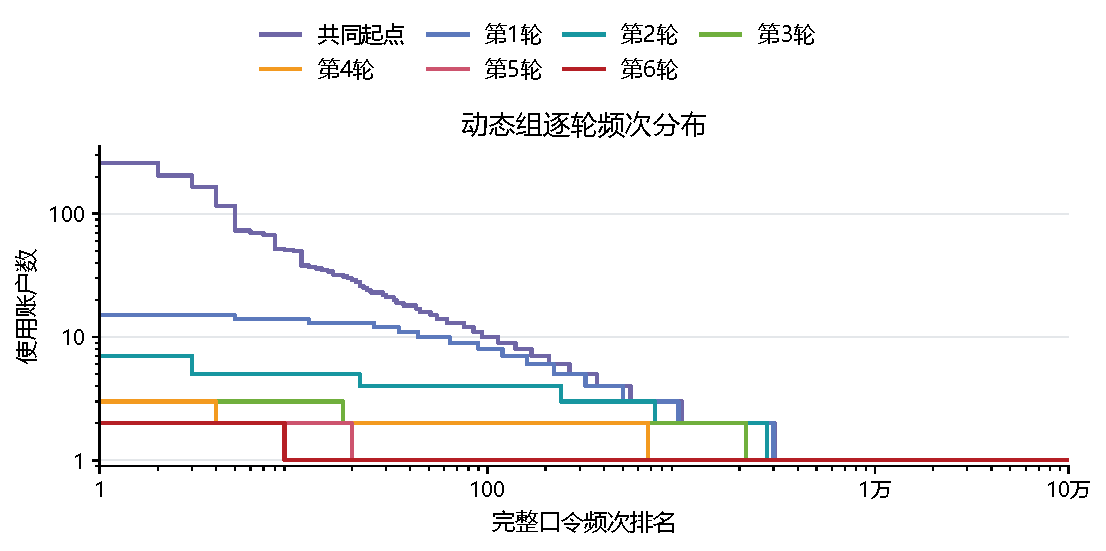
\includegraphics[width=\linewidth]{validation_3_1_rounds.pdf}
\caption{\quad 动态组逐轮完整口令频次分布；排名与频次均采用对数刻度}\label{fig:validation-existing-1}
\end{figure}

\subsubsection{实验二：与HTPG方法的对比}\label{sec:validation-existing-htpg}

采用HTPG方法在本项目统一下的补全实现\cite{xiao2022zipf}与动态策略比较，两组从相同10万账户的8字符状态运行6轮，使用相同双模型猜测预算。HTPG按论文比例响应，后续修改1,255.574次期望事件；动态组全部成功修改12,000次。结果见图\ref{fig:validation-existing-htpg}：动态组W1为0.000071，低于HTPG的0.037883；F、A1联合命中率为8.096\%、9.613\%，分别比HTPG的16.013\%、18.489\%低7.917、8.876个百分点。动态策略取得了更分散的分布和更低的攻击命中率。证明我们的方案有更高的安全性。

\begin{figure}[H]
\centering
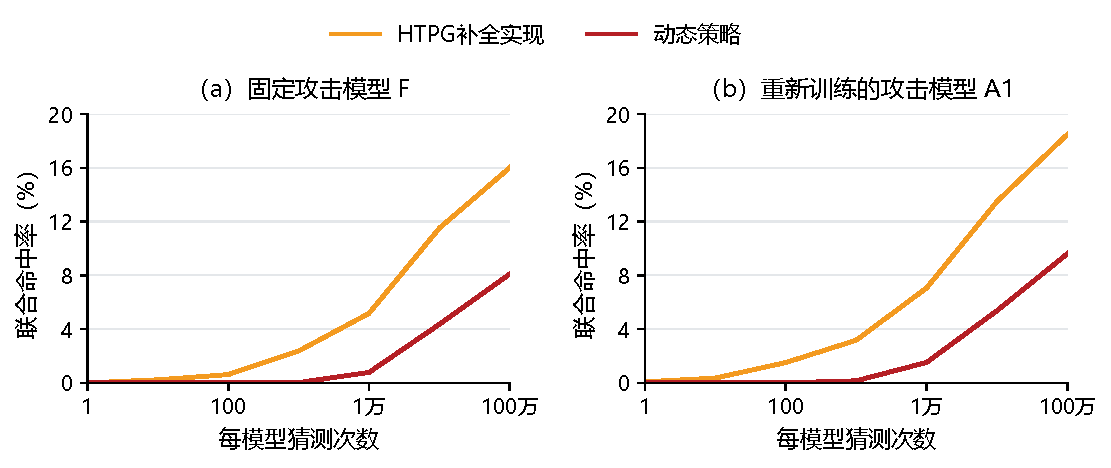
\includegraphics[width=\linewidth]{validation_3_1_htpg.pdf}
\caption{\quad 实验二中HTPG与动态策略在F、A1下的联合命中率；每模型采用相同猜测预算}\label{fig:validation-existing-htpg}
\end{figure}

% BEGIN VALIDATION 3.2

\subsection{模拟注册阶段口令策略动态调整方案验证}\label{sec:validation-registration}

本节评价第\ref{sec:design-registration}节的动态口令策略调整方法，设置对照为Schechter\cite{schechter2010popularity}、Malone--Maher\cite{malone2012distribution}、固定Segreti整类结构名单\cite{segreti2017diversify}及GitHub公开核心规则\cite{github2026password}，重点比较相同样本和实际猜测预算下的攻击命中率。

\subsubsection{实验设置}\label{sec:validation-registration-settings}

目标样本共100,000个模拟用户，按10批、每批10,000人注册，种子为11。开发训练、选择预览与确认预览分别为60,000、10,000、10,000条，出现位置互不重叠，字符串可重复；每次选择与确认各预览3,000人。

Schechter采用热门口令频率阈值$10^{-5}$\cite{schechter2010popularity}；Malone--Maher按频次概率拒绝\cite{malone2012distribution}；固定Segreti从首批执行213种结构名单\cite{segreti2017diversify}。前三种方法与本作品共用至少8位及开发训练前1,000个常见口令禁用要求，动态组与固定Segreti的初始名单和首批结果一致。GitHub采用公开核心要求：至少15位，或至少8位且有小写字母与数字\cite{github2026password}。

五组共用目标与开发分区，各组用60,000条开发训练记录按相应策略重选后的口令训练PCFG与OMEN，每模型实际猜测100万次，联合最多200万次；重复猜测占用次数，账户命中计一次，分母为全部100,000个初始模拟用户。用户持续重选至策略接受，重选成本以首次提交后的人均额外提交次数表示。

\subsubsection{五种策略的攻击结果}\label{sec:validation-registration-attacks}

表\ref{tab:registration-version-selection}汇总五种策略的最终攻击结果，图\ref{fig:registration-five-policy-comparison}展示不同猜测预算下的联合命中率。本作品动态策略的PCFG、OMEN和联合命中率均为五组最低。

\begin{table}[H]
\centering
\caption{五种策略的最终攻击结果（每模型100万次猜测）}\label{tab:registration-version-selection}
\small
\begin{tabularx}{\linewidth}{@{}Xrrrr@{}}
\toprule
方法 & PCFG & OMEN & 联合 & \shortstack{两模型\\均不支持} \\
\midrule
动态策略 & 8.803\% & 1.157\% & 8.992\% & 0.889\% \\
Schechter（严格） & 18.818\% & 6.231\% & 22.322\% & 0.354\% \\
Malone--Maher & 23.221\% & 8.504\% & 27.362\% & 0.339\% \\
固定Segreti名单 & 9.231\% & 1.346\% & 9.431\% & 0.853\% \\
GitHub公开核心规则 & 27.619\% & 11.476\% & 29.749\% & 0.536\% \\
\bottomrule
\end{tabularx}
\end{table}

动态方法联合命中率为8.992\%，较固定Segreti的9.431\%低0.439个百分点，单模型也均下降。OMEN补充命中189个PCFG未命中的账户。

\begin{figure}[H]
\centering
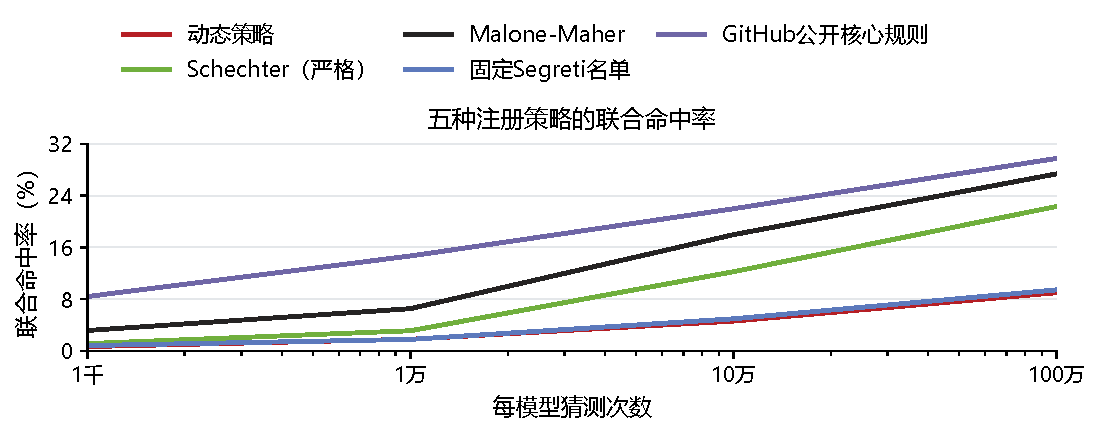
\includegraphics[width=\linewidth]{registration_five_policy_comparison.pdf}
\caption{五种注册策略的联合命中率；横轴为每模型猜测次数，合计最多为其两倍}\label{fig:registration-five-policy-comparison}
\end{figure}

若将总计100万次平均分给两模型，即每模型各50万次，本作品与固定Segreti的联合命中率分别为7.373\%和7.803\%，差0.430个百分点。

\subsubsection{动态名单变化}\label{sec:validation-registration-timeline}

表\ref{tab:registration-timeline}展示动态策略在十批注册过程中的名单变化，包括追加、保持与恢复三种决策。

\begin{table}[H]
\centering
\caption{动态策略在十批注册过程中的结构名单变化}\label{tab:registration-timeline}
\small
\begin{tabularx}{\linewidth}{@{}rrX@{}}
\toprule
注册批次 & 阻断结构数 & 本批采用的决策 \\
\midrule
1 & 213 & 执行原始Segreti名单 \\
2 & 213 & 保持当前名单 \\
3 & 218 & 确认后追加结构 \\
4--6 & 218 & 保持当前名单 \\
7 & 213 & 恢复原始Segreti名单 \\
8 & 233 & 确认后追加结构 \\
9 & 253 & 确认后追加结构 \\
10 & 273 & 确认后追加结构 \\
\bottomrule
\end{tabularx}
\end{table}

第3批候选在选择与确认中使预计联合命中率分别下降0.177778、0.077778个百分点，因而启用；第6批选择结果下降0.016667个百分点，确认结果却增加0.033333个百分点，因而保持名单。这两批结果展示了独立确认对名单更新的作用。

\subsubsection{注册完成情况与重选成本}\label{sec:validation-registration-cost}

五组均完成100,000个模拟用户的注册。动态策略的人均额外提交为2.66616次，固定Segreti名单为2.34561次，平均增加0.32055次。

% END VALIDATION 3.2



% BEGIN VALIDATION 3.3
\setcounter{subsection}{2}
\subsection{面向动态策略口令状态统计中的隐私保护方案验证}\label{sec:validation-privacy}

本节验证第\ref{sec:design-privacy}节的秘密输入、结构与匿名频次计算，以及差分隐私发布机制。实验直接对照测试输入、协议返回、统计数值和预算记录，分别检查输入的一致性、计算的正确性与发布参数的执行情况。

\subsubsection{验证设置与安全条件}\label{sec:validation-privacy-1}

实验采用8个初始合成账户：\texttt{atlas2026!}出现3次，\texttt{audit2026!}、\texttt{Breeze742!}、\texttt{Quartz816?}、\texttt{rivertrail88}和\texttt{Moonlight74!}各出现1次。客户端分别上传随机份额，由三个计算进程完成协议；新增账户后总人数为9。测试程序用这些已知口令计算参考值，并在受控测试中记录加噪前的实际统计，对外发布加噪后的汇总结果。配置见表\ref{tab:privacy-validation-settings}。

\begin{table}[H]
\centering
\caption{三方协议验证的实验设置}\label{tab:privacy-validation-settings}
\small
\begin{tabularx}{\linewidth}{@{}lX@{}}
\toprule
项目 & 设置 \\
\midrule
账户与输入 & 初始8个、最终9个合成账户；口令固定填充至16字节 \\
统计范围 & 4种公开结构及OTHER，共5桶；每桶前3项匿名频次，共20维 \\
协议与通信 & MPyC 0.11；三方秘密分享；双向认证TLS分别上传份额 \\
发布预算 & 每次新发布$\varepsilon=1$，累计上限2；另核对$\varepsilon=0.5,1,2$的噪声参数 \\
运行环境 & 同一台机器上的三个独立计算进程 \\
\bottomrule
\end{tabularx}
\end{table}

安全条件为客户端可信、三方分别由独立主体管理；至多一方被攻击者控制，且各方仍按协议执行。单方份额与秘密输入无关的代数依据见第\ref{sec:design-privacy}节。

\subsubsection{秘密输入与检查的一致性验证}\label{sec:validation-privacy-2}

同一口令\texttt{Sunbeam482\#}以不同随机数分享两次，两次认证均返回成功。每方分别接收128个秘密位的份额，表\ref{tab:privacy-share-values}列出首个位置的实际值；三方各自的128个位置在两次分享中均发生变化。

\begin{table}[H]
\centering
\caption{同一口令两次分享的实际份额值}\label{tab:privacy-share-values}
\small
\begin{tabular}{@{}lrrr@{}}
\toprule
接收方 & 首次分享的首个值 & 再次分享的首个值 & 不同位置数 \\
\midrule
计算方1 & 227696167922352513 & 159614073195965826 & 128 \\
计算方2 & 167161959692993338 & 30997770240219964 & 128 \\
计算方3 & 106627751463634163 & 190611843436185789 & 128 \\
\bottomrule
\end{tabular}
\end{table}

认证、结构推导和规则检查使用同一秘密输入。测试的结构限制为\texttt{L5D4S1}，匿名热门项对应\texttt{Breeze742!}。表\ref{tab:privacy-protocol-checks}对照明文命中标记（1命中、0未命中）与三方返回。

\begin{table}[H]
\centering
\caption{测试输入、明文规则判断与实际协议结果}\label{tab:privacy-protocol-checks}
\small
\begin{tabularx}{\linewidth}{@{}Xcc l@{}}
\toprule
测试输入或操作 & \shortstack{结构\\命中} & \shortstack{热门\\命中} & 三方返回 \\
\midrule
\texttt{atlas2026!} & 1 & 0 & 拒绝注册 \\
\texttt{Breeze742!} & 0 & 1 & 拒绝注册 \\
\texttt{Delta395?} & 0 & 0 & 注册成功 \\
仅将第三方首个份额增加1 & -- & -- & 份额检查拒绝 \\
三方首个份额均增加1，使秘密位由1变为2 & -- & -- & 位值检查拒绝 \\
提交\texttt{A}、零填充后再提交非零字符 & -- & -- & 格式检查拒绝 \\
额外上报结构字段\texttt{L1} & -- & -- & 字段检查拒绝 \\
额外提交不同的认证口令\texttt{tiny} & -- & -- & 字段检查拒绝 \\
\bottomrule
\end{tabularx}
\end{table}

改密后再用旧口令\texttt{Quartz816?}认证，返回失败；用新口令\texttt{Sunbeam482\#}认证，返回成功。三个计算方各自的4个JSON文件及1份计算日志均未出现测试口令字符串。公开统计包含快照、预算、账户总数、结构人数和匿名频次，没有口令字符串或逐账户结构。

\subsubsection{秘密结构与匿名频次的正确性验证}\label{sec:validation-privacy-3}

表\ref{tab:privacy-secret-statistics}逐桶对照初始状态的明文参考与三方计算值。每格按“人数，前3项频次”排列：同口令的重复计入频次，同结构的不同口令分列，不足3项补零。五桶共20项数值的最大绝对误差为0。

\begin{table}[H]
\centering
\caption{初始状态的明文参考与秘密统计实际值}\label{tab:privacy-secret-statistics}
\small
\begin{tabular}{@{}lccr@{}}
\toprule
结构 & 明文参考 & 三方计算 & 最大绝对误差 \\
\midrule
L5D4S1 & $(4,3,1,0)$ & $(4,3,1,0)$ & 0 \\
U1L5D3S1 & $(2,1,1,0)$ & $(2,1,1,0)$ & 0 \\
L10D2 & $(1,1,0,0)$ & $(1,1,0,0)$ & 0 \\
U1L8D2S1 & $(1,1,0,0)$ & $(1,1,0,0)$ & 0 \\
OTHER & $(0,0,0,0)$ & $(0,0,0,0)$ & 0 \\
\bottomrule
\end{tabular}
\end{table}

随后依次新增\texttt{Delta395?}，测试失败改密，再执行三次成功改密：\texttt{Quartz816?}改为\texttt{Sunbeam482\#}、\texttt{atlas2026!}改为\texttt{Meadow953\#}、\texttt{Delta395?}改为\texttt{Meadow953\#}。表\ref{tab:privacy-statistic-updates}列出每次操作前后的实际结构人数，顺序与表\ref{tab:privacy-secret-statistics}相同；最后一列为全部20项统计的$L_1$变化量。

\begin{table}[H]
\centering
\caption{注册、改密与重复请求前后的实际统计变化}\label{tab:privacy-statistic-updates}
\small
\begin{tabular}{@{}lccr@{}}
\toprule
操作 & 操作前结构人数 & 操作后结构人数 & $L_1$变化 \\
\midrule
新增账户 & $(4,2,1,1,0)$ & $(4,2,1,1,1)$ & 2 \\
失败改密 & $(4,2,1,1,1)$ & $(4,2,1,1,1)$ & 0 \\
首次成功改密 & $(4,2,1,1,1)$ & $(4,1,1,1,2)$ & 4 \\
重发同一改密请求 & $(4,1,1,1,2)$ & $(4,1,1,1,2)$ & 0 \\
第二次成功改密 & $(4,1,1,1,2)$ & $(3,2,1,1,2)$ & 4 \\
第三次成功改密 & $(3,2,1,1,2)$ & $(3,3,1,1,1)$ & 4 \\
\bottomrule
\end{tabular}
\end{table}

第三次成功改密将两个账户合并到同一口令，\texttt{U1L5D3S1}的频次由$(1,1,0)$变为$(2,1,0)$，OTHER由$(1,1,0)$变为$(1,0,0)$。各阶段20项统计均与明文参考一致，重载前后最大绝对差为0；失败改密和重发请求的统计向量均不变。

\subsubsection{差分隐私发布机制验证}\label{sec:validation-privacy-4}

固定6个账户，枚举6种口令、2种结构、每桶前2项频次的462个分布状态，并逐一替换一个账户口令。表\ref{tab:privacy-sensitivity-values}列出7,560对相邻状态的实际$L_1$变化分布，同结构替换最大为2，跨结构替换最大为4，与第\ref{sec:design-privacy}节的敏感度上界一致。

\begin{table}[H]
\centering
\caption{单账户口令替换后的统计变化分布（状态对数）}\label{tab:privacy-sensitivity-values}
\small
\begin{tabular}{@{}lrrrrrr@{}}
\toprule
替换类型 & 变化0 & 变化1 & 变化2 & 变化3 & 变化4 & 合计 \\
\midrule
同结构 & 960 & 864 & 1,200 & 0 & 0 & 3,024 \\
跨结构 & 0 & 0 & 72 & 1,152 & 3,312 & 4,536 \\
\bottomrule
\end{tabular}
\end{table}

协议的20维发布使用实际采样函数计算几何参数$q$。三档预算下，$q$分别约为0.8824969026、0.7788007831和0.6065306597；对应的$-4\log q$均不超过0.5、1和2。参数以64位分母向上舍入，采样上界为$M=2^{28}$。各方每维生成两个几何样本之差，在秘密计算内合成三份独立噪声，至少一份噪声保持私密。共120个几何样本的有限采样尾项为
\[
\tau\leq120q^M,\qquad \delta\leq(1+e^{\varepsilon})\tau.
\]
负数修正、排序和人数范围限制在加噪后执行。

表\ref{tab:privacy-release-checks}列出每次发布前后的实际累计预算。两次缓存重读与各自首次发布结果逐项比较，最大绝对差均为0；快照14的发布被拒绝，没有生成新的公开统计。

\begin{table}[H]
\centering
\caption{统计发布的快照与实际预算记录}\label{tab:privacy-release-checks}
\small
\begin{tabular}{@{}l c c l@{}}
\toprule
操作 & 快照编号 & 累计预算：前$\rightarrow$后 & 协议结果 \\
\midrule
首次发布 & 8 & $0\rightarrow 1$ & 返回新统计 \\
重读首个快照 & 8 & $1\rightarrow 1$ & 返回缓存 \\
发布新快照 & 13 & $1\rightarrow 2$ & 返回新统计 \\
重读新快照 & 13 & $2\rightarrow 2$ & 返回缓存 \\
预算耗尽后发布 & 14 & $2\rightarrow 2$ & 拒绝发布 \\
\bottomrule
\end{tabular}
\end{table}

\subsubsection{验证小结}\label{sec:validation-privacy-5}

实际输入与规则判断一致，各结构人数及匿名频次与明文参考逐项相同。成功改密正确移除旧贡献并加入新贡献，失败改密和重复请求的统计变化量为0。相邻状态的最大$L_1$变化为4；新快照按次扣减预算，同快照读取保持结果与预算不变，预算耗尽后拒绝发布。
% END VALIDATION 3.3


% BEGIN PERFORMANCE 3.4
\subsection{性能测试}\label{sec:performance}

TriGuard由管理员网站、用户浏览器插件、业务服务和三个计算方组成。用户通过插件完成口令检查、登录与修改，管理员通过网站查看受保护统计并设置口令要求。因此，系统的工程性能既取决于常用操作的响应时间，也受到三方统计计算与账户数据存储开销的影响。本作品在保留秘密分享、加密通信、签名核验和事务恢复机制的基础上，采用计算结果复用与无损数据压缩降低运行开销，并对用户操作的时间开销及受保护统计的决策效用进行测试。

\subsubsection{时间开销}\label{sec:performance-time}

登录、口令检查和改密是用户直接参与的操作，其执行时间会影响使用体验；群体统计则需要处理多个账户的秘密输入，计算开销相对较大。为减少运行开销，本作品采用精确分块比较复用口令匹配结果，仅秘密选取所需的热门项，避免对全部候选进行完整排序；同时复用字符类型和连续序列检查的中间结果，并省去登录、检查过程中整份账户状态的复制与无变化写回。

本作品依据实际使用场景开展以下测试：

\begin{enumerate}
\item 在100个合成账户的站点中，分别对登录、私密口令检查和改密进行预热后的5次测量。计时从客户端发起操作开始，覆盖策略与版本读取、请求签发、份额生成与提交、三方计算、回执核验和业务完成，采用中位数表示典型耗时。
\item 在10个合成账户的站点中，对不同数据快照进行3次全量统计发布。每次均由三个计算方处理普通逐账户秘密份额，发布结构人数、结构内匿名热门频次及18类规则人数统计，单次隐私预算为0.5，采用3次测量的中位数表示统计发布耗时。
\end{enumerate}

实验在同一台机器上运行三个独立计算进程，通过HTTPS完成业务交互。各次统计发布均实际执行秘密计算与加噪过程。测试结果如下表所示。

\begin{table}[H]
\centering
\begin{tabular}{lr}
\toprule
操作 & 中位耗时 / 秒 \\
\midrule
用户登录 & 0.927 \\
私密口令检查 & 1.761 \\
用户改密 & 1.928 \\
\bottomrule
\end{tabular}
\end{table}

结果表明，在本机测试条件下，三项用户交互操作的中位耗时均低于2秒，能够以秒级响应完成私密认证、规则检查和凭据更新，时间开销较小。


% END PERFORMANCE 3.4

\clearpage
\section{创新性说明}\label{ux7b2cux56dbux7ae0-ux521bux65b0ux6027ux8bf4ux660e}

本作品围绕网站的口令管理，完成了“已有口令集分布动态调整方案”、“模拟注册阶段口令策略动态调整方案”、“面向动态策略口令状态统计中的隐私保护方案”、“网站口令管理助手与用户口令辅助选取工具”四个部分。各部分分别解决“先让谁改、让新用户怎么选、不看明文怎样统计、怎样真正执行”的问题。本章说明这些部分的具体改进，以及它们之间的联系。

\subsection{已有口令集分布动态调整方案}\label{sec:innovation-1}

本部分面向已有账户，在通知人数约束下，把完整口令分布、修改对象和修改要求接入逐轮决策。其创新集中在以下三个方面。

\textbf{联合选择修改对象、修改要求和通知人数。}先识别热门完整口令和相似结构的使用群体，再模拟不同要求作用后的分布，在人数预算内比较各项安排，使有限的修改机会用于预计改善较大的群体。

\textbf{依据修改后的实际分布逐轮更新决策。}每轮执行后重新统计口令分布和剩余通知人数，并据此选择下一轮动作，使后续安排反映已经发生的变化，避免始终沿用起点时的账户排序。

\textbf{衔接群体分散程度与新口令抗猜测检查。}以“每个账户使用一个不同口令”为分散程度的参照，用归一化对数排名上的一维Wasserstein-1距离比较调整安排；候选新口令另行接受PCFG和马尔可夫模型检查。当前实验要求新口令在两个模型各自前100万次猜测中均未被命中，并至少处于一个模型能够评价的范围内，使分布改善与个体口令检查共同约束修改方案。

第\ref{sec:validation-existing}节在共同起点和相同逐轮通知人数下比较随机选择、初始排序和动态调整，用于区分定向选择与反馈更新的作用。

\subsection{模拟注册阶段口令策略动态调整方案}\label{sec:innovation-2}

本部分在已有热门口令限制与整类结构阻断研究\cite{schechter2010popularity,segreti2017diversify}上，提出保留完整基础名单、用双模型确认决定是否追加限制的动态流程。其创新集中在以下三个方面。

\textbf{保留可比较、可恢复的基础名单。}首批即执行完整Segreti名单，每轮把原始名单和当前名单同时纳入评价。新增候选必须优于两者中更好的可行方案，才有资格进入确认；确认未通过时，可保持当前要求或恢复原始名单。

\textbf{以攻击者重新学习后的累计风险决定更新。}系统先模拟用户重选，再用重选后的独立开发口令训练PCFG与OMEN，同时评价历史账户和下一批账户。整类结构限制针对常见选取模式，双模型评价进一步检查替代口令是否仍能被结构和连续字符规律猜中，使决策直接面向规则执行后的防御效果。

\textbf{把再次确认和风险转移检查纳入执行流程。}选择与确认使用不同预览角色，新增规则在两次评价中均降低联合命中率才启用；固定攻击集合和模型支持检查另行排除明显风险转移。系统接受小幅正向改善，并保留每轮名单、攻击结果和决策依据，使追加、保持及恢复均可复核。

第\ref{sec:validation-registration}节在相同名单起点与攻击预算下，观察到本方法的联合命中率较固定Segreti下降0.439个百分点，PCFG与OMEN单模型命中率也同时降低。这支持本次模拟条件下整套动态流程的额外防御价值。

\subsection{面向动态策略口令状态统计中的隐私保护方案}\label{sec:innovation-3}

本部分面向不收集明文口令的策略调整，设计保留结构归属的匿名统计表示，并将其与联合限制和隐藏规则执行连接起来。其创新集中在以下三个方面。

\textbf{按结构保留热门口令的匿名名次和频次。}管理员可以查看结构人数及每个结构内的热门口令频次，真实字符串与匿名位置的对应关系留在三方安全计算内部。相较于分别给出全局频次和结构总人数，这种表示保留了两类热门信息的对应关系，为判断规则覆盖是否重叠提供依据。

\textbf{在联合限制中排除重复覆盖。}先确定被禁结构，再从其他结构中补充热门完整口令，使已经被结构规则覆盖的热点不再占用完整口令名额，减少两类限制对同一批账户的重复覆盖。

\textbf{将匿名统计选择与隐藏规则执行衔接。}用户通过可信客户端分别上传随机份额，结构由同一个秘密口令推导，避免依赖用户另报的标签。管理员选择结构与匿名位置，由三方在安全计算内部完成实际字符串检查，无须下载热门口令的明文名单。

秘密分享、安全计算和差分隐私采用已有方法，本部分的贡献是上述统计表示及其与策略执行的衔接。输入保护与统计发布分别处理：前者保护口令及秘密中间值，后者对公开人数和频次加噪，并累计发布预算。

第\ref{sec:validation-privacy}节评价匿名统计的效用及协议实现。条件画像保留的信息更多，也增加了噪声负担，现有实验并未显示它在所有隐私预算下都更准确。结构外选择的覆盖性质也不等于重选后的攻击效果一定更好。隐私保证需要可信客户端、独立三方和至多一方被动腐化等条件。

\subsection{网站口令管理助手与用户口令辅助选取工具}\label{sec:innovation-4}

本作品将前面的方案接成用户浏览器扩展和独立管理员网站，并提供网站登录接入样例。用户在扩展内选取口令、注册、登录、改密和处理本人任务；管理员查看受保护统计、设置要求、安排整改和核对完成情况。两端使用分开的身份、会话与存储，必要的策略、本人任务和受保护汇总通过后端按权限传递。

工具接入的关键是让实际口令、规则检查和统计更新保持一致。注册成功才增加贡献，改密成功替换旧贡献，失败和重复请求不额外计数；整改通知发出后仍为待处理，只有真实改密成功才计完成。网站根据三方签署的认证结果建立自己的会话，管理员不用查看口令字符串，也不能用界面操作代替用户完成修改。

这一部分属于围绕本项目方法的工程整合：把受保护统计、策略设置、秘密检查和实际完成反馈连接起来，为前面三部分提供可操作的使用路径。普通浏览器扩展、角色隔离和任务管理本身不作为新算法。当前已有本地合成数据验收；真实用户响应、跨机构部署和大规模容量仍需进一步验证。缺少本站响应模型与成本确认时，自动候选保持当前策略，管理员手动应用限制也与自动决策分别记录。

\clearpage
\section{总结与后续工作}\label{ux7b2cux4e94ux7ae0-ux603bux7ed3ux4e0eux540eux7eedux5de5ux4f5c}

\subsection{工作总结}\label{ux5de5ux4f5cux603bux7ed3}

本作品完成了“已有口令集分布动态调整方案”、“模拟注册阶段口令策略动态调整方案”、“面向动态策略口令状态统计中的隐私保护方案”、“网站口令管理助手与用户口令辅助选取工具”四个部分，分别解决“优先让谁修改”“后续用户怎样选择”“不看明文怎样掌握热门情况”和“怎样实际执行”的问题。

\subsection{当前局限}\label{ux5f53ux524dux5c40ux9650}

首先，实验数据和用户行为与真实网站仍有差距。泄露语料中的出现记录未被核实为独立真实账户，同源数据划分也不能代替跨网站验证。已有账户实验把收到通知后成功改密作为设定，部分新口令由程序补全；注册实验的重选方式同样来自行为假设，不设次数上限并假定用户持续尝试至接受，未测真人退出和沮丧。注册比较属于探索性模拟，尚未进行独立样本验证。因此，攻击命中率下降说明的是这些设定下的效果，不能直接推算真人的接受率、记忆负担或长期使用情况。已有账户主实验仅有一次种子运行，其小幅优势也需要重复核对。

策略搜索限于给定的规则、群体和预览规模，攻击评价使用PCFG、OMEN及固定猜测预算。后续需增加规则范围、独立样本和攻击类型。

隐私方案要求可信客户端、独立三方；至多一方受攻击者控制，且仍按协议执行。统计采用固定结构目录和有限热门频次，保护固定人数下单账户口令替换的统计发布；参与身份、检查结果和任务状态另需保护。完整分布距离计算和双模型训练目前仍在离线数据上进行。

工具测试使用本地合成账户，跨机构运行和并发容量需要补充测试。一次7账户统计确认发布耗时约200秒，秘密计算开销仍较高。

\subsection{后续工作}\label{ux540eux7eedux5de5ux4f5c}

后续首先补充真实操作反馈。Komanduri等和Tan等的用户研究分别提供了组成政策及组合要求的评价思路，Ur等的数据驱动口令强度提示研究则为设计可理解、可操作的反馈提供参考\cite{komanduri2011people,tan2020minimumstrength,ur2017meter}。本作品计划在适当授权下开展小规模研究，检查用户对拒绝提示的理解、口令记忆、改密完成和恢复行为，用实测结果校准当前响应假设。注册过程保留未完成记录，避免只观察成功者；提示是否改善安全与体验均由后续实测判断。

使用独立来源数据和多个随机种子重复实验，增加不同重选假设与神经网络猜测模型\cite{ur2015guessability,melicher2016neural}。

完善注册、改密和持续发布的隐私统计流程，在统一预算下比较发布周期、误差和延迟\cite{dwork2010continual,naor2019password}。进一步研究秘密状态下的分布距离和攻击风险计算，连接统计接口与自动策略选择。

开展独立三方部署，测试网络延迟、并发、故障恢复和批处理开销。参考SPDZ方案研究对偏离协议行为的检查\cite{damgard2012spdz}，评估OPAQUE口令认证协议与恢复、三方统计的衔接\cite{rfc9807opaque}；结合工具测试检查权限、重复请求、中断恢复及隐藏名单下的提示效果。

\clearpage
\phantomsection
\addcontentsline{toc}{section}{参考文献}
\renewcommand{\refname}{参考文献}
\begin{thebibliography}{99}

\bibitem{bonneau2012quest} BONNEAU J, HERLEY C, VAN OORSCHOT P C, et al. The Quest to Replace Passwords: A Framework for Comparative Evaluation of Web Authentication Schemes[C]//2012 IEEE Symposium on Security and Privacy. 2012: 553--567. DOI: \href{https://doi.org/10.1109/SP.2012.44}{10.1109/SP.2012.44}.

\bibitem{florencio2014password} FLORÊNCIO D, HERLEY C, VAN OORSCHOT P C. An Administrator's
Guide to Internet Password Research{[}C{]}//28th Large Installation
System Administration Conference. 2014: 35--52.
\href{https://www.usenix.org/conference/lisa14/conference-program/presentation/florencio}{会议出版页}.

\bibitem{komanduri2011people} KOMANDURI S, SHAY R, KELLEY P G, et al. Of Passwords and People: Measuring the Effect of Password-Composition Policies[C]//Proceedings of the SIGCHI Conference on Human Factors in Computing Systems. New York: ACM, 2011: 2595--2604. DOI: \href{https://doi.org/10.1145/1978942.1979321}{10.1145/1978942.1979321}.

\bibitem{bonneau2012science} BONNEAU J. The Science of Guessing: Analyzing an Anonymized Corpus of 70 Million Passwords[C]//2012 IEEE Symposium on Security and Privacy. 2012: 538--552. DOI: \href{https://doi.org/10.1109/SP.2012.49}{10.1109/SP.2012.49}.

\bibitem{wang2017zipf} WANG D, CHENG H, WANG P, et al. Zipf's Law in Passwords{[}J{]}.
IEEE Transactions on Information Forensics and Security, 2017, 12(11): 2776--2791. DOI:
\href{https://doi.org/10.1109/TIFS.2017.2721359}{10.1109/TIFS.2017.2721359}.

\bibitem{hou2023observations} HOU Z, WANG D. New Observations on Zipf's Law in Passwords{[}J{]}.
IEEE Transactions on Information Forensics and Security, 2023, 18: 517--532. DOI:
\href{https://doi.org/10.1109/TIFS.2022.3176185}{10.1109/TIFS.2022.3176185}.

\bibitem{johnson2020skeptic} JOHNSON S, FERREIRA J F, MENDES A, et al. Skeptic: Automatic,
Justified and Privacy-Preserving Password Composition Policy Selection{[}C{]}//
Proceedings of the 15th ACM Asia Conference on Computer and Communications Security.
2020: 101--115. DOI:
\href{https://doi.org/10.1145/3320269.3384762}{10.1145/3320269.3384762}.

\bibitem{xiao2022zipf} XIAO Y, ZENG J. Dynamically Generate Password Policy via Zipf
Distribution{[}J{]}. IEEE Transactions on Information Forensics and
Security, 2022, 17: 835--848. DOI:
\href{https://doi.org/10.1109/TIFS.2022.3152357}{10.1109/TIFS.2022.3152357}.

\bibitem{zhu2023fepg} 朱浩, 郭华, 陈晨, 等. 一种基于频率和熵的口令策略生成框架{[}J{]}.
网络空间安全科学学报, 2023, 1(2): 73--82.
\href{https://www.journalofcybersec.com/EN/Y2023/V1/I2/73}{期刊出版页}.

\bibitem{schechter2010popularity} SCHECHTER S, HERLEY C, MITZENMACHER M. Popularity Is Everything: A New Approach to Protecting Passwords from Statistical-Guessing Attacks[C]//5th USENIX Workshop on Hot Topics in Security (HotSec 10). USENIX Association, 2010. \href{https://www.usenix.org/conference/hotsec10/popularity-everything-new-approach-protecting-passwords-statistical-guessing}{会议出版页}.

\bibitem{malone2012distribution} MALONE D, MAHER K. Investigating the Distribution of Password Choices[C]//Proceedings of the 21st International Conference on World Wide Web. 2012: 301--310.
\href{https://www.maths.tcd.ie/~dwmalone/p/www2012.pdf}{作者提供的论文全文}.

\bibitem{tan2020minimumstrength} TAN J, BAUER L, CHRISTIN N, et al. Practical Recommendations for Stronger, More Usable Passwords Combining Minimum-strength, Minimum-length, and Blocklist Requirements[C]//Proceedings of the 2020 ACM SIGSAC Conference on Computer and Communications Security. New York: ACM, 2020: 1407--1426. DOI: \href{https://doi.org/10.1145/3372297.3417882}{10.1145/3372297.3417882}.

\bibitem{segreti2017diversify} SEGRETI S M, MELICHER W, KOMANDURI S, et al. Diversify to Survive: Making Passwords Stronger with Adaptive Policies[C]//Thirteenth Symposium on Usable Privacy and Security (SOUPS 2017). USENIX Association, 2017: 1--12. \href{https://www.usenix.org/conference/soups2017/technical-sessions/presentation/segreti}{会议出版页}.

\bibitem{blocki2016frequency} BLOCKI J, DATTA A, BONNEAU J. Differentially Private Password Frequency Lists{[}C{]}//Network and Distributed System Security Symposium. 2016. DOI:
\href{https://doi.org/10.14722/ndss.2016.23328}{10.14722/ndss.2016.23328}.

\bibitem{naor2019password} NAOR M, PINKAS B, RONEN E. How to (not) Share a Password: Privacy Preserving Protocols for Finding Heavy Hitters with Adversarial Behavior[C]//Proceedings of the 2019 ACM SIGSAC Conference on Computer and Communications Security. New York: ACM, 2019: 1369--1386. DOI: \href{https://doi.org/10.1145/3319535.3363204}{10.1145/3319535.3363204}.

\bibitem{weir2009pcfg} WEIR M, AGGARWAL S, DE MEDEIROS B, et al. Password Cracking
Using Probabilistic Context-Free Grammars{[}C{]}//2009 30th IEEE
Symposium on Security and Privacy. 2009: 391--405. DOI:
\href{https://doi.org/10.1109/SP.2009.8}{10.1109/SP.2009.8}.

\bibitem{durmuth2015omen} DÜRMUTH M, ANGELSTORF F, CASTELLUCCIA C, et al. OMEN: Faster Password Guessing Using an Ordered Markov Enumerator{[}C{]}//Engineering Secure Software and Systems. Cham: Springer, 2015: 119--132. DOI:
\href{https://doi.org/10.1007/978-3-319-15618-7_10}{10.1007/978-3-319-15618-7\_10}.

\bibitem{melicher2016neural} MELICHER W, UR B, SEGRETI S M, et al. Fast, Lean, and Accurate: Modeling Password Guessability Using Neural Networks[C]//25th USENIX Security Symposium. USENIX Association, 2016: 175--191. \href{https://www.usenix.org/conference/usenixsecurity16/technical-sessions/presentation/melicher}{会议出版页}.

\bibitem{ur2015guessability} UR B, KELLEY P G, KOMANDURI S, et al. Measuring Real-World
Accuracies and Biases in Modeling Password Guessability{[}C{]}//24th
USENIX Security Symposium. 2015: 463--481.
\href{https://www.usenix.org/conference/usenixsecurity15/technical-sessions/presentation/ur}{会议出版页}.

\bibitem{panaretos2019wasserstein} PANARETOS V M, ZEMEL Y. Statistical Aspects of Wasserstein
Distances{[}J{]}. Annual Review of Statistics and Its Application, 2019,
6: 405--431. DOI:
\href{https://doi.org/10.1146/annurev-statistics-030718-104938}{10.1146/annurev-statistics-030718-104938}.

\bibitem{shamir1979secret} SHAMIR A. How to Share a Secret[J]. Communications of the ACM, 1979, 22(11): 612--613. DOI: \href{https://doi.org/10.1145/359168.359176}{10.1145/359168.359176}.

\bibitem{benor1988mpc} BEN-OR M, GOLDWASSER S, WIGDERSON A. Completeness Theorems for Non-Cryptographic Fault-Tolerant Distributed Computation[C]//Proceedings of the Twentieth Annual ACM Symposium on Theory of Computing. New York: ACM, 1988: 1--10. DOI: \href{https://doi.org/10.1145/62212.62213}{10.1145/62212.62213}.

\bibitem{mpycsoftware} SCHOENMAKERS B. MPyC: Multiparty Computation in Python{[}EB/OL{]}. {[}2026-10-11{]}.
\href{https://github.com/lschoe/mpyc}{项目仓库与安全模型说明}.

\bibitem{rfc2104hmac} KRAWCZYK H, BELLARE M, CANETTI R. HMAC: Keyed-Hashing for Message Authentication: RFC 2104[R]. RFC Editor, 1997. DOI: \href{https://doi.org/10.17487/RFC2104}{10.17487/RFC2104}.

\bibitem{dwork2014privacy} DWORK C, ROTH A. The Algorithmic Foundations of Differential Privacy{[}J{]}. Foundations and Trends in Theoretical Computer Science, 2014, 9(3--4): 211--407. DOI:
\href{https://doi.org/10.1561/0400000042}{10.1561/0400000042}.

\bibitem{github2026password} GITHUB. Creating a strong password[EB/OL]. [2026-10-11].
\href{https://docs.github.com/en/authentication/keeping-your-account-and-data-secure/creating-a-strong-password}{GitHub官方说明}.

% References supporting the privacy design in section 2.1.3.

\bibitem{ur2017meter} UR B, ALFIERI F, AUNG M, et al. Design and Evaluation of a Data-Driven Password Meter[C]//Proceedings of the 2017 CHI Conference on Human Factors in Computing Systems. New York: ACM, 2017: 3775--3786. DOI: \href{https://doi.org/10.1145/3025453.3026050}{10.1145/3025453.3026050}.

\bibitem{dwork2010continual} DWORK C, NAOR M, PITASSI T, et al. Differential Privacy under Continual Observation[C]//Proceedings of the Forty-Second ACM Symposium on Theory of Computing. New York: ACM, 2010: 715--724. DOI: \href{https://doi.org/10.1145/1806689.1806787}{10.1145/1806689.1806787}.

\bibitem{damgard2012spdz} DAMGÅRD I, PASTRO V, SMART N P, et al. Multiparty Computation from Somewhat Homomorphic Encryption[C]//Advances in Cryptology--CRYPTO 2012. Berlin, Heidelberg: Springer, 2012: 643--662. DOI: \href{https://doi.org/10.1007/978-3-642-32009-5_38}{10.1007/978-3-642-32009-5\_38}.

\bibitem{rfc9807opaque} BOURDREZ D, KRAWCZYK H, LEWI K, et al. The OPAQUE Augmented Password-Authenticated Key Exchange (aPAKE) Protocol: RFC 9807[R]. RFC Editor, 2025. DOI: \href{https://doi.org/10.17487/RFC9807}{10.17487/RFC9807}.

\bibitem{google2026password} GOOGLE. Create a strong password \& a more secure
account{[}EB/OL{]}. {[}2026-10-08{]}.
\href{https://support.google.com/accounts/answer/32040}{Google Account
Help}.

\bibitem{yahoo2026policy} YAHOO! JAPAN. Yahoo! JAPAN
IDに{\reportjapanese 関}するヘルプ：H000004639{[}EB/OL{]}. {[}2026-10-08{]}.
\href{https://support.yahoo-net.jp/SccLogin/s/article/H000004639}{帮助页面}.

\end{thebibliography}

\appendix
\renewcommand{\thetable}{\Alph{section}-\arabic{table}}
\ctexset{appendix/number={附录\space\Alph{section}}}
\titleformat{\section}[block]{\reportkai\fontsize{18}{27}\selectfont\bfseries}{附录\space\Alph{section}}{0.8em}{}
\renewcommand{\thesubsection}{\Alph{section}.\arabic{subsection}}
\renewcommand{\thesubsubsection}{\Alph{section}.\arabic{subsection}.\arabic{subsubsection}}
\clearpage
\section{完整修改方法池与来源说明}\label{ux9644ux5f55-a-ux5b8cux6574ux4feeux6539ux65b9ux6cd5ux6c60ux4e0eux6765ux6e90ux8bf4ux660e}

\subsection{完整 20 条方法}\label{a.1-ux5b8cux6574-20-ux6761ux65b9ux6cd5}

表\ref{tab:rule-catalogue}列出从 Top20 网站口令政策资料中提取并归并的 20
条修改方法。编号是报告与实现之间的对照约定，不表示网站排名，也不表示 20
条规则必须同时启用。最低 6 字符和最低 8
字符已由共同起点满足，因此后续局部调整默认使用其余 18 条。

{
\setlength{\LTcapwidth}{\linewidth}
\small
\begin{longtable}[]{@{}>{\raggedright\arraybackslash}p{(\linewidth - 4\tabcolsep) * \real{0.32}}>{\raggedright\arraybackslash}p{(\linewidth - 4\tabcolsep) * \real{0.27}}>{\raggedright\arraybackslash}p{(\linewidth - 4\tabcolsep) * \real{0.41}}@{}}
\caption{完整 20 条修改方法}\label{tab:rule-catalogue}\\
\toprule\noalign{}
编号 & 修改方法 & 后续角色 \\
\midrule\noalign{}
\endfirsthead
\caption[]{完整 20 条修改方法（续）}\\
\toprule\noalign{}
编号 & 修改方法 & 后续角色 \\
\midrule\noalign{}
\endhead
\bottomrule\noalign{}
\endlastfoot
1 & 长度至少 10 字符 & 默认局部候选 \\
2 & 长度至少 12 字符 & 默认局部候选 \\
3 & 长度至少 15 字符 & 默认局部候选 \\
4 & 至少一个英文字母 & 默认局部候选 \\
5 & 至少一个小写英文字母 & 默认局部候选 \\
6 & 至少一个大写英文字母 & 默认局部候选 \\
7 & 至少一个数字 & 默认局部候选 \\
8 & 至少一个数字或符号 & 默认局部候选 \\
9 & 大写、小写、数字、符号至少两类 & 默认局部候选 \\
10 & 至少四个不同字符 & 默认局部候选 \\
11 & 禁止连续三个相同字符 & 默认局部候选 \\
12 & 禁止整串为同一字符 & 默认局部候选 \\
13 & 禁止简单键盘序列 & 默认局部候选 \\
14 & 禁止四位连续字母或数字顺序序列 & 默认局部候选 \\
15 & 禁止仅为开发词表中的字典词 & 默认局部候选 \\
16 & 禁止包含固定可预测词 & 默认局部候选 \\
17 & 禁止当前热门完整口令 & 默认局部候选 \\
18 & 禁止命中独立开发样本中的泄露口令 & 默认局部候选 \\
19 & 长度至少 6 字符 & 已由共同起点满足 \\
20 & 长度至少 8 字符 & 已由共同起点满足 \\
\end{longtable}
}

部分规则会影响同一账户，搜索时按实际覆盖人数与修改结果比较。

\subsection{网站条款与实现来源}\label{a.2-ux7f51ux7ad9ux6761ux6b3eux4e0eux5b9eux73b0ux6765ux6e90}

网站政策资料是修改方法的直接来源，研究论文用于支持分布建模、政策优化和攻击评估的理论背景，二者承担不同引用职责。规则整理过程对语义相同的条款进行归并，并将依赖用户名、姓名、历史口令或网站专有字段而无法在现有数据上判定的要求排除在默认候选之外。

实验的8字符基础规则只检查长度。Google帮助页另包含避免弱口令、历史复用和使用更长口令等建议\cite{google2026password}。Yahoo! JAPAN对照按保存的条款摘要执行长度、允许字符和禁止组合要求\cite{yahoo2026policy}，从原始状态进行一次全站迁移。项目保存页面快照、采集日期和规则对应关系。

\clearpage
\section{参数、记账与复现说明}\label{ux9644ux5f55-b-ux53c2ux6570ux8bb0ux8d26ux4e0eux590dux73b0ux8bf4ux660e}

\subsection{主要参数}\label{b.1-ux4e3bux8981ux53c2ux6570}

已有账户实验的参数按用途分列：表\ref{tab:existing-data-budget}给出数据规模、通知预算与响应条件，表\ref{tab:existing-search-fitting}给出候选搜索与分布拟合设置，表\ref{tab:existing-generation-checks}给出候选复核、攻击模型和新口令生成设置。复现时需同时使用这三部分参数。

{
\setlength{\LTcapwidth}{\linewidth}
\small
\begin{longtable}[]{@{}>{\raggedright\arraybackslash}p{(\linewidth - 4\tabcolsep) * \real{0.32}}>{\raggedright\arraybackslash}p{(\linewidth - 4\tabcolsep) * \real{0.27}}>{\raggedright\arraybackslash}p{(\linewidth - 4\tabcolsep) * \real{0.41}}@{}}
\caption{已有账户实验的数据、预算与响应参数}\label{tab:existing-data-budget}\\
\toprule\noalign{}
参数 & 设定 & 说明 \\
\midrule\noalign{}
\endfirsthead
\caption[]{已有账户实验的数据、预算与响应参数（续）}\\
\toprule\noalign{}
参数 & 设定 & 说明 \\
\midrule\noalign{}
\endhead
\bottomrule\noalign{}
\endlastfoot
目标账户数 & 100,000 & 固定规模模拟群体 \\
开发参考出现记录 & 100,000 & 训练、调参与验证角色相互分离 \\
单轮后续通知上限 & 2,000 & 目标账户数的 2\% \\
后续总通知上限 & 20,000 & 目标账户数的 20\% \\
候选批次比例 & 0.1\%、0.2\%、0.5\%、1\%、2\% & 用于比较不同动作规模 \\
每模型个体门槛 & 1,000,000 次 & PCFG 与 马尔可夫模型 分别检查 \\
用户响应 & 全部成功修改 & 无未响应与失败账户 \\
随机种子 & 42 & 固定抽样与模拟顺序 \\
\end{longtable}
}

{
\setlength{\LTcapwidth}{\linewidth}
\small
\begin{longtable}[]{@{}>{\raggedright\arraybackslash}p{(\linewidth - 4\tabcolsep) * \real{0.32}}>{\raggedright\arraybackslash}p{(\linewidth - 4\tabcolsep) * \real{0.27}}>{\raggedright\arraybackslash}p{(\linewidth - 4\tabcolsep) * \real{0.41}}@{}}
\caption{已有账户实验的搜索与拟合参数}\label{tab:existing-search-fitting}\\
\toprule\noalign{}
参数 & 设定 & 作用 \\
\midrule\noalign{}
\endfirsthead
\caption[]{已有账户实验的搜索与拟合参数（续）}\\
\toprule\noalign{}
参数 & 设定 & 作用 \\
\midrule\noalign{}
\endhead
\bottomrule\noalign{}
\endlastfoot
热门完整口令数 & 20 & 构造头部候选群体 \\
重点群体上限 & 12 & 控制单轮候选规模 \\
初筛候选数 & 80 & 保留跨结构及随机候选 \\
组合搜索宽度 & 6 & 比较有限的不重叠子动作组合 \\
前瞻宽度/预演次数 & 2/2 & 普通搜索失败后的有限检查 \\
CDF 拟合样本数 & 100,000 & 与目标规模一致 \\
独立再采样次数 & 5 & 复核最大累计误差 \\
\end{longtable}
}

{
\setlength{\LTcapwidth}{\linewidth}
\small
\begin{longtable}[]{@{}>{\raggedright\arraybackslash}p{(\linewidth - 4\tabcolsep) * \real{0.32}}>{\raggedright\arraybackslash}p{(\linewidth - 4\tabcolsep) * \real{0.27}}>{\raggedright\arraybackslash}p{(\linewidth - 4\tabcolsep) * \real{0.41}}@{}}
\caption{已有账户实验的候选复核与安全生成参数}\label{tab:existing-generation-checks}\\
\toprule\noalign{}
参数 & 取值 & 作用 \\
\midrule\noalign{}
\endfirsthead
\caption[]{已有账户实验的候选复核与安全生成参数（续）}\\
\toprule\noalign{}
参数 & 取值 & 作用 \\
\midrule\noalign{}
\endhead
\bottomrule\noalign{}
\endlastfoot
马尔可夫阶数 & 3 & 固定字符序列模型设置 \\
响应预测次数 & 3 & 候选初筛中的响应模拟 \\
候选复核次数 & 5 & 计算候选平均分布收益 \\
拟合 W1 独立采样次数 & 3 & 给定拟合参数下计算距离，与拟合误差复核区分 \\
普通候选正收益容差 & $10^{-12}$ & 区分预计改善与数值误差 \\
前瞻首步经验分布损失上限 & 0.0003 & 限制首步暂时损失 \\
常规提案尝试上限 & 5 & 未通过时进入规则补全与安全重生成 \\
安全随机补全构造上限 & 128 & 用尽后仍未通过则整批方案不下发 \\
\end{longtable}
}

\subsection{注册策略的参数与复现}\label{app:registration-reproduction}

本节只对应第二板块，不沿用表\ref{tab:existing-data-budget}、表\ref{tab:existing-search-fitting}和表\ref{tab:existing-generation-checks}中的已有账户通知预算或种子42。现行配置为\texttt{\seqsplit{registration\_segreti\_dynamic\_full.json}}，入口为\texttt{\seqsplit{run\_registration\_segreti\_dynamic.py}}，参数见表\ref{tab:registration-parameters}。

\begin{table}[H]
\centering
\caption{最终注册方法的主要参数}\label{tab:registration-parameters}
\small
\begin{tabularx}{\linewidth}{@{}lX@{}}
\toprule
参数 & 设定 \\
\midrule
目标与批次 & 100,000条出现记录，10批，每批10,000条，种子11 \\
开发角色 & 训练60,000条，选择预览10,000条，确认预览10,000条 \\
每次模拟预览 & 选择、确认各3,000人，使用不同预览角色 \\
共同基础要求 & 至少8位，拒绝开发训练前1,000个常见口令 \\
原始结构名单 & 同一份Segreti名单，213种结构，从首批执行 \\
每轮候选 & 原始名单、当前名单及分别追加5或20种结构的名单 \\
近期统计与偏好 & 最近2批；开发记录与历史首次提议各占一半 \\
新增结构排序 & 使用人数至少20，人数降序，同人数按结构编码 \\
重选方式比例 & 局部修改60\%，片段拼接25\%，重新选取15\% \\
选择、确认与攻击 & PCFG、OMEN各1,000,000次实际猜测 \\
更新收益要求 & 两次累计联合命中率均优于更好的可行基准；容差$10^{-12}$ \\
固定风险检查 & 相对原始名单，命中比例增量不超过0.5个百分点 \\
模型支持检查 & 相对原始名单，两模型均不支持的增量不超过2个百分点 \\
用户重选条件 & 不设次数上限，持续重选至接受 \\
实际执行结构数 & 首批213种，最后一批273种；允许恢复原始名单 \\
\bottomrule
\end{tabularx}
\end{table}

复现时读取保存的目标、开发分区及Segreti名单，检查文件哈希；建立固定双模型集合$F$，逐批完成候选构造、选择、确认和注册。所有执行名单保留原始213种结构，首批结果与固定Segreti一致。最后用各组开发用户重选后的口令训练PCFG和OMEN，统计实际猜测次数、命中率、模型支持和额外提交。导出入口为\texttt{\seqsplit{report\_registration\_segreti\_dynamic.py}}。

更新要求是选择与确认均有正向改善；0.5个百分点用于固定风险增量检查。预览中的原始名单按已发生的累计开发历史评价。模拟用户持续重选至接受。

\subsection{已有账户调整的成本账本}\label{b.2-ux6210ux672cux8d26ux672c}

账本分别保存基础迁移修改数、后续通知事件数、累计不同通知账户数、累计不同修改账户数和修改事件数。基础迁移与后续局部调整可能再次作用于同一账户，因此两个阶段的修改事件之和可以大于累计不同修改账户数。

生成候选未通过要求时继续尝试，所有正式通知均成功完成修改，未响应和最终不合规人数均为0。

\subsection{已有账户调整的复现顺序}\label{b.3-ux590dux73b0ux987aux5e8f}

\begin{enumerate}
\def\labelenumi{\arabic{enumi}.}
\item
  核对语料文件摘要、编码和有效出现次数，读取保存的实验配置。
\item
  按固定种子抽取互不重叠的目标与开发出现位置，保存各角色摘要。
\item
  使用开发训练角色建立固定 PCFG 与 OMEN，各实际猜测100万次。
\item
  构造 8 字符基础规则共同起点，并检查三个局部组的账户级状态一致。
\item
  运行动态组，逐轮保存群体、规则、通知人数、个体门槛和分布变化。
\item
  按动态组的实际逐轮通知人数运行随机分批组和初始排序组。
\item
  对每组独立参考迁移结果训练 A1，计算 PCFG、OMEN 与猜测并集曲线。
\item
  运行账户规模、共同起点、通知预算、个体门槛和最终状态结果审计，导出图表。
\end{enumerate}

语料按Latin-1读取，共扫描14,344,391行，其中10行解析失败，有效出现次数为32,603,039。复现时使用一致的语料、配置、种子、源码和上游模型；结果文件保存摘要、计数、曲线与模型来源。

\subsection{已有账户实验的补充结果}\label{app:existing-additional-results}

以下保留实验一的拟合距离、单模型命中率和模型支持情况，以及实验二的完整分布与攻击结果。HTPG按50\%保持、25\%第一建议、25\%第二建议计算变化，未成功改写的分支保留原口令；F与动态组使用相同猜测，A1用同一60,000账户的独立参考起点各自修改后重新训练。

\begin{table}[H]
\centering
\caption{已有账户各组的完整分布指标}\label{tab:existing-full-distribution}
\small
\begin{tabular}{@{}>{\raggedright\arraybackslash}p{(\linewidth - 8\tabcolsep) * \real{0.2100}}>{\raggedright\arraybackslash}p{(\linewidth - 8\tabcolsep) * \real{0.1800}}>{\raggedright\arraybackslash}p{(\linewidth - 8\tabcolsep) * \real{0.1800}}>{\raggedright\arraybackslash}p{(\linewidth - 8\tabcolsep) * \real{0.1800}}>{\raggedright\arraybackslash}p{(\linewidth - 8\tabcolsep) * \real{0.2500}}@{}}
\toprule
组别 & 不同口令数 & 经验W1 & 拟合W1 & 经验距离较共同起点下降 \\
\midrule
原始组 & 82,840 & 0.086247 & 0.090194 & — \\
8字符基础规则 & 92,495 & 0.040946 & 0.041021 & 0.00\% \\
随机分批 & 93,741 & 0.034866 & 0.034840 & 14.85\% \\
固定策略 & 99,963 & 0.000284 & 0.000245 & 99.31\% \\
动态调整 & 99,992 & 0.000071 & 0.000057 & 99.83\% \\
\bottomrule
\end{tabular}
\end{table}

\begin{table}[H]
\centering
\caption{固定模型F的百万次预算结果}\label{tab:existing-fixed-attack}
\small
\begin{tabular}{@{}>{\raggedright\arraybackslash}p{(\linewidth - 8\tabcolsep) * \real{0.2100}}>{\raggedright\arraybackslash}p{(\linewidth - 8\tabcolsep) * \real{0.1800}}>{\raggedright\arraybackslash}p{(\linewidth - 8\tabcolsep) * \real{0.1800}}>{\raggedright\arraybackslash}p{(\linewidth - 8\tabcolsep) * \real{0.1800}}>{\raggedright\arraybackslash}p{(\linewidth - 8\tabcolsep) * \real{0.2500}}@{}}
\toprule
组别 & PCFG命中率 & OMEN命中率 & 并集命中率 & 两模型均不支持的账户比例 \\
\midrule
原始组 & 31.404\% & 15.806\% & 36.900\% & 0.385\% \\
8字符基础规则 & 16.251\% & 2.053\% & 16.627\% & 11.802\% \\
随机分批 & 14.302\% & 1.811\% & 14.637\% & 10.407\% \\
固定策略 & 8.312\% & 0.545\% & 8.632\% & 11.597\% \\
动态调整 & 7.769\% & 0.549\% & 8.096\% & 11.669\% \\
\bottomrule
\end{tabular}
\end{table}

\begin{table}[H]
\centering
\caption{适应性模型A1的百万次预算结果}\label{tab:existing-adaptive-attack}
\small
\begin{tabular}{@{}>{\raggedright\arraybackslash}p{(\linewidth - 8\tabcolsep) * \real{0.2100}}>{\raggedright\arraybackslash}p{(\linewidth - 8\tabcolsep) * \real{0.1800}}>{\raggedright\arraybackslash}p{(\linewidth - 8\tabcolsep) * \real{0.1800}}>{\raggedright\arraybackslash}p{(\linewidth - 8\tabcolsep) * \real{0.1800}}>{\raggedright\arraybackslash}p{(\linewidth - 8\tabcolsep) * \real{0.2500}}@{}}
\toprule
组别 & PCFG命中率 & OMEN命中率 & 并集命中率 & 两模型均不支持的账户比例 \\
\midrule
原始组 & 31.404\% & 15.806\% & 36.900\% & 0.385\% \\
8字符基础规则 & 18.621\% & 2.940\% & 19.058\% & 1.967\% \\
随机分批 & 16.132\% & 2.355\% & 16.472\% & 1.758\% \\
固定策略 & 9.727\% & 0.582\% & 10.046\% & 1.935\% \\
动态调整 & 9.247\% & 0.656\% & 9.613\% & 1.960\% \\
\bottomrule
\end{tabular}
\end{table}

\begin{table}[H]
\centering
\caption{同一起点、六轮后的分布与修改规模}\label{tab:htpg-distribution-cost}
\small
\begin{tabular}{@{}>{\raggedright\arraybackslash}p{(\linewidth - 8\tabcolsep) * \real{0.2700}}>{\raggedright\arraybackslash}p{(\linewidth - 8\tabcolsep) * \real{0.1000}}>{\raggedright\arraybackslash}p{(\linewidth - 8\tabcolsep) * \real{0.1800}}>{\raggedright\arraybackslash}p{(\linewidth - 8\tabcolsep) * \real{0.2000}}>{\raggedright\arraybackslash}p{(\linewidth - 8\tabcolsep) * \real{0.2500}}@{}}
\toprule
方案 & 轮数 & 不同口令数 & W1距离 & 后续修改事件 \\
\midrule
共同8字符起点 & 0 & 92,495 & 0.040946 & 0 \\
HTPG补全实现 & 6 & 92,550 & 0.037883 & 1,255.574（期望值） \\
本作品动态调整 & 6 & 99,992 & 0.000071 & 12,000 \\
\bottomrule
\end{tabular}
\end{table}

\begin{table}[H]
\centering
\caption{HTPG补全实现与本作品的双模型攻击结果}\label{tab:htpg-dual-attack}
\small
\begin{tabular}{@{}>{\raggedright\arraybackslash}p{(\linewidth - 8\tabcolsep) * \real{0.1200}}>{\raggedright\arraybackslash}p{(\linewidth - 8\tabcolsep) * \real{0.2800}}>{\raggedright\arraybackslash}p{(\linewidth - 8\tabcolsep) * \real{0.2000}}>{\raggedright\arraybackslash}p{(\linewidth - 8\tabcolsep) * \real{0.2000}}>{\raggedright\arraybackslash}p{(\linewidth - 8\tabcolsep) * \real{0.2000}}@{}}
\toprule
评价条件 & 方案 & PCFG命中率 & OMEN命中率 & 并集命中率 \\
\midrule
F & HTPG补全实现 & 15.637\% & 1.403\% & 16.013\% \\
F & 本作品动态调整 & 7.769\% & 0.549\% & 8.096\% \\
A1 & HTPG补全实现 & 18.037\% & 2.349\% & 18.489\% \\
A1 & 本作品动态调整 & 9.247\% & 0.656\% & 9.613\% \\
\bottomrule
\end{tabular}
\end{table}

\clearpage
\section{实验记录与证据索引}\label{ux9644ux5f55-c-ux5b9eux9a8cux8bb0ux5f55ux4e0eux8bc1ux636eux7d22ux5f15}

表\ref{tab:reproduction-evidence}列出已有账户实验的运行标识和输入来源。

{
\setlength{\LTcapwidth}{\linewidth}
\begin{longtable}[]{@{}
  >{\raggedright\arraybackslash}p{(\linewidth - 4\tabcolsep) * \real{0.3333}}
  >{\raggedright\arraybackslash}p{(\linewidth - 4\tabcolsep) * \real{0.3333}}
  >{\raggedright\arraybackslash}p{(\linewidth - 4\tabcolsep) * \real{0.3333}}@{}}
\caption{实验记录与复现标识}\label{tab:reproduction-evidence}\\
\toprule\noalign{}
\begin{minipage}[b]{\linewidth}\raggedright
项目
\end{minipage} & \begin{minipage}[b]{\linewidth}\raggedright
记录
\end{minipage} & \begin{minipage}[b]{\linewidth}\raggedright
用途
\end{minipage} \\
\midrule\noalign{}
\endfirsthead
\caption[]{实验记录与复现标识（续）}\\
\toprule\noalign{}
\begin{minipage}[b]{\linewidth}\raggedright
项目
\end{minipage} & \begin{minipage}[b]{\linewidth}\raggedright
记录
\end{minipage} & \begin{minipage}[b]{\linewidth}\raggedright
用途
\end{minipage} \\
\midrule\noalign{}
\endhead
\bottomrule\noalign{}
\endlastfoot
实验运行标识 & \texttt{3a83057341104cfc} & 定位结构化报告与图表目录 \\
目标账户 & 100,000 & 第三章分布、成本和攻击结果 \\
开发出现记录 & 100,000 & 固定攻击模型与独立参考迁移 \\
语料 SHA-256 &
\texttt{\seqsplit{e9d22d5316e7668aba2e9fa1c22dfc6e5afd217a60defc8f3c7f68a4f48f84b9}}
& 识别输入数据 \\
PCFG 固定提交 & \texttt{\seqsplit{b04bbdadfe8928fd1287fa73ad1aa46a297ff83a}} & 识别
PCFG 实现 \\
OMEN 固定提交 & \texttt{\seqsplit{10aa99e30bb88a10052d389feb53f739254eb1d1}} &
识别作者版 OMEN 实现 \\
随机种子 & 42 & 复现抽样与模拟顺序 \\
运行时间 & 2,290.02 秒 & 记录当前计算代价 \\
\end{longtable}
}

程序检查通过了账户规模、共同8字符起点、逐轮通知匹配、单轮2,000人及总计20,000人的通知上限、新口令双模型百万猜测门槛和最终A1评价。

注册实验记录标识为\texttt{\seqsplit{registration\_segreti\_dynamic\_20261012}}，四个外部对照为\texttt{\seqsplit{registration\_dual\_full\_20261011}}。各组使用相同目标与开发分区，目标规模100,000条、种子11，每模型实际猜测100万次。动态方法与固定Segreti使用相同原始名单，首批目标、开发结果及重选顺序逐项一致。

正文图表来自保存的实验记录。图\ref{fig:validation-existing-2}汇总五组内部对照，图\ref{fig:validation-existing-1}展示逐轮完整口令频次分布，图\ref{fig:validation-existing-htpg}比较HTPG与动态策略。其他单模型曲线和拟合参数图保存在项目实验目录。

\end{document}
